% This is a LaTeX thesis template for Adam Mickiewicz University.
% to be used with quarto
% This template was produced by Jakub Nowosad
% Version: 22 July 2023

% Inspired by:
% This is a LaTeX thesis template for Monash University.
% to be used with Rmarkdown
% This template was produced by Rob Hyndman
% Version: 6 September 2016

\documentclass{amuthesis}
% \usepackage[polish]{babel}
\usepackage{polski}
\renewcommand{\figurename}{Rycina} % Redefine default figure caption %
\renewcommand{\tablename}{Tabela} % Redefine default table caption %
%%%%%%%%%%%%%%%%%%%%%%%%%%%%%%%%%%%%%%%%%%%%%%%%%%%%%%%%%%%%%%%
% Add any LaTeX packages and other preamble here if required
%%%%%%%%%%%%%%%%%%%%%%%%%%%%%%%%%%%%%%%%%%%%%%%%%%%%%%%%%%%%%%%
\usepackage{booktabs,tabularx} % Allows kableExtra to work %
\usepackage{indentfirst} % Adds indent in the first paragraph %
\usepackage{bookmark} % Adds indent in the first paragraph %
\usepackage{float}

\author{Filip Ratajszczak}
\title{Wykrywanie farm fotowoltaicznych na podstawie danych
teledetekcyjnych}
\def\titleeng{Detection of photovoltaic farms based on remote sensing
data}
\def\degreetitle{Praca inżynierska}
\def\major{Geoinformacja}
\def\albumid{461791}
\def\thesisyear{2024}

% Add subject and keywords below
\hypersetup{
     %pdfsubject={The Subject},
     %pdfkeywords={Some Keywords},
     pdfauthor={Filip Ratajszczak},
     pdftitle={Wykrywanie farm fotowoltaicznych na podstawie danych
teledetekcyjnych},
     pdfproducer={quarto with LaTeX}
}

\bibliography{thesis.bib, packages.bib}

\begin{document}

\pagenumbering{arabic}

\titlepage

\bookmarksetup{startatroot}

\hypertarget{streszczenie}{%
\chapter*{Streszczenie}\label{streszczenie}}
\addcontentsline{toc}{chapter}{Streszczenie}

\markboth{Streszczenie}{Streszczenie}

\textbf{Abstrakt}

Energia pozyskiwana z odnawialnych źródeł odgrywa kluczową rolę w
ograniczaniu emisji gazów cieplarnianych do atmosfery. Szybki wzrost
liczby wielkoskalowych instalacji fotowoltaicznych, czyli farm
fotowoltaicznych, powoduje konieczność monitorowania ich ilości i
lokalizacji w celu analizy postępów w tym sektorze energetyki
odnawialnej. Celem pracy było określenie optymalnych metod wykrywania
farm fotowoltaicznych na podstawie danych teledetekcyjnych. W procesie
detekcji wykorzystano dane radarowe z misji Sentinel-1 oraz dane
multispektralne z misji Sentinel-2, wraz z ich pochodnymi, takimi jak
wskaźniki teledetekcyjne i tekstury obrazu. Na podstawie tych zmiennych
dokonano uczenia i walidacji kilku modeli lasów losowych (ang.
\emph{Random Forest}) w celu wskazania optymalnej konfiguracji
predyktorów. Uzyskane wyniki potwierdziły możliwość detekcji farm
fotowoltaicznych na podstawie danych teledetekcyjnych. Najlepsze
rezultaty w końcowej klasyfikacji po procesie przetwarzania końcowego
osiągnął model oparty na kanałach Sentinel-2 oraz wykorzystanych
wskaźnikach teledetekcyjnych (NDVI, NDBI i mNDWI). Po przetwarzaniu
końcowym model ten wykazał precyzję na poziomie 87\% i czułość na
poziomie 84\%, co przełożyło się na ostateczny wynik 85\% dla miary
F1-score. Dodatkowo badanie wykazało, że dane radarowe z misji
Sentinel-1 i ich pochodne nie były istotne w procesie detekcji farm
fotowoltaicznych. Wyniki badania mogą stanowić podstawę dla przyszłych
prac nad monitorowaniem rozwoju farm fotowoltaicznych w Polsce.

Słowa kluczowe: odnawialne źródła energii, dane satelitarne, pokrycie
terenu i użytkowania ziemi, uczenie maszynowe, lasy losowe, klasyfikacja
obrazu

\newpage

\textbf{Abstract}

Energy derived from renewable sources plays a crucial role in reducing
the emission of greenhouse gases into the atmosphere. The rapid growth
in the number of large-scale photovoltaic installations, commonly known
as solar farms, necessitates the monitoring of their quantity and
locations for the analysis of progress in this renewable energy sector.
The goal of this study was to determine optimal methods for detecting
photovoltaic farms based on remote sensing data. The detection process
utilized radar data from the Sentinel-1 mission and multispectral data
from the Sentinel-2 mission, along with their derivatives, such as
spectral indices and image textures. Several Random Forest models were
trained and validated using these variables to indicate the optimal
predictor configuration. The obtained results confirmed the possibility
of detecting photovoltaic farms based on remote sensing data. The best
results in the final classification after the post-processing were
achieved by the model based on Sentinel-2 channels and the spectral
indices used (NDVI, NDBI, and mNDWI). After post-processing, this model
demonstrated precision at the level of 87\% and sensitivity at the level
of 84\%, which resulted in a final result of 85\% for the F1-score
measure. Furthermore, the study showed that radar data from the
Sentinel-1 mission and their derivatives were not important in the
process of detecting photovoltaic farms. The study results may
constitute the basis for future work on monitoring the development of
photovoltaic farms in Poland.

Keywords: renewable energy sources, satellite data, land use and land
cover, machine learning, random forests, image classification

\newpage

\setstretch{1.2}\sf\tighttoc\doublespacing

\bookmarksetup{startatroot}

\hypertarget{sec-wprowadzenie}{%
\chapter{Wprowadzenie}\label{sec-wprowadzenie}}

Energia elektryczna odgrywa kluczową rolę w życiu większości ludzi,
stanowiąc podstawę funkcjonowania społeczeństwa i napędzając rozwój
gospodarczy \autocite{iea2021}. Istnieje wiele metod pozyskiwania
energii elektrycznej, włączając w to tradycyjne, konwencjonalne sposoby
oparte na spalaniu paliw kopalnych, a także energię atomową oraz
odnawialne źródła energii (OZE). Odnawialne źródła energii, określane
inaczej jako zielona energia, wykorzystują naturalne procesy, takie jak
promieniowanie słoneczne, siła wiatru czy ciepło wnętrza Ziemi, w celu
generowania energii elektrycznej.

Zasoby surowców wykorzystywanych do produkcji energii konwencjonalnej są
ograniczone. Statystyczny przegląd światowej energetyki
(\emph{Statistical Review of World Energy}) opracowany przez firmę BP w
2021 roku wskazuje, że obecne zasoby paliw kopalnych, takich jak ropa
naftowa, gaz ziemny i węgiel, wystarczą odpowiednio na 50, 48,8 i 139
lat przy utrzymaniu obecnego poziomu produkcji
\autocite{bp_2021_world_energy}. Dodatkowo, rosnące zainteresowanie
ochroną środowiska i negatywnymi skutkami zmian klimatu oraz wprowadzane
przepisy prawne zobowiązują do podejmowania działań mających na celu
ograniczenie emisji szkodliwych gazów do atmosfery. W obliczu globalnych
zmian klimatycznych i kryzysu energetycznego, spowodowanego między
innymi inwazją Rosji na Ukrainę w 2022 roku, społeczeństwo jest zmuszone
do przejścia z produkcji energii opartej na paliwach kopalnych na rzecz
odnawialnych źródeł energii i energetyki jądrowej
\autocite{iea2021,iea2022}.

Ambitne cele klimatyczne Unii Europejskiej, których podstawę stanowi
Europejski Zielony Ład (ang. \emph{European Green Deal}), sprawiają, że
energia elektryczna pochodząca z odnawialnych źródeł energii zaczyna
odgrywać kluczową rolę w procesie transformacji energetycznej Unii
Europejskiej. Europejski Zielony Ład to zestaw inicjatyw politycznych
mających na celu przeprowadzenie transformacji ekologicznej i
osiągnięcie neutralności klimatycznej w UE do 2050 roku
\autocite{european_green_deal}. Inicjatywy takie jak Gotowi na 55 (ang.
\emph{Fit For 55}) oraz rozporządzenie o europejskim prawie klimatycznym
mają zapewnić redukcję emisji gazów cieplarnianych o co najmniej 55\% do
2030 roku \autocite{european_green_deal}. Jednocześnie, zgodnie z
ustaleniami Rady Unii Europejskiej, Parlamentu Europejskiego oraz
Komisji Europejskiej, udział energii odnawialnej w ogólnym zużyciu
energii w Unii Europejskiej ma wynosić 42,5\% do 2030 roku
\autocite{renewable_energy_eu}. Inną inicjatywą organów Unii
Europejskiej jest plan REPowerEU, czyli unijny plan transformacji
energetycznej i uniezależnienia od rosyjskich paliw kopalnych
przedstawiony przez Komisję Europejską w maju 2022 roku
\autocite{repowerEU2022}. Przedsięwzięcie to skupia się na inwestycjach
w odnawialne źródła energii, zakładając uruchomienie niemal 600 GW mocy
nowych instalacji fotowoltaicznych w całej Unii Europejskiej do 2030
roku \autocite{repowerEU2022}. Działania te uznaje się za kluczowe z
punktu widzenia interesu publicznego.

Osiągnięcie wymienionych celów będzie możliwe jedynie poprzez dokładne
monitorowanie wyników działań oraz posiadanie aktualnych informacji
dotyczących odnawialnych źródeł energii. Transformacja energetyczna jest
dynamicznym procesem, którego monitorowanie będzie miało znaczący wpływ
na rozwój kolejnych projektów z zakresu energetyki odnawialnej.
Niejednolita organizacja działania władz samorządowych w Polsce oraz
występowanie na terenie kraju różnych operatorów energetycznych utrudnia
jednak śledzenie rozwoju polskiej branży OZE. W oficjalnych, dostępnych
w Polsce źródłach danych brakuje aktualnych informacji na temat
lokalizacji elektrowni słonecznych. Wśród nieoficjalnych źródeł danych
informacje na ten temat można znaleźć m.in. w projekcie społeczności
internetowej OpenStreetMap \autocite{OpenStreetMap}, gdzie są one
oznaczone jako \texttt{tag:plant:source=solar}, jednak dane te są
nieformalne, niepełne i zazwyczaj nieaktualne. W związku z brakiem
jednolitych danych na temat lokalizacji farm fotowoltaicznych w
oficjalnych źródłach w Polsce, wykorzystanie danych satelitarnych staje
się potencjalnym narzędziem do ich detekcji, umożliwiając pozyskiwanie
aktualnych informacji na ten temat. Obserwacje satelitarne pozwalają
również regularnie monitorować rozwój farm fotowoltaicznych, co
umożliwia analizę postępów w tym sektorze energetyki odnawialnej.

Na przestrzeni ostatnich kilku lat podejmowano kilka prób detekcji farm
fotowoltaicznych na podstawie danych teledetekcyjnych przy wykorzystaniu
metod uczenia maszynowego. \textcite{kruitwagen_2021_pv}, wykorzystując
zdjęcia satelitarne SPOT-6/7 i Sentinel-2 w połączeniu z metodami
uczenia maszynowego, wskazał istniejące farmy fotowoltaiczne na świecie
na dzień 30 września 2018 roku. Inne badania, takie jak te
przeprowadzone przez Zhanga et al. \autocite*{zhang_2021_texture},
Plakman et al. \autocite*{plakman_2022_pv} i Wanga et al.
\autocite*{wang_2022_pv}, również koncentrowały się na detekcji
instalacji fotowoltaicznych, lecz nie obejmowały obszaru Polski.

Celem niniejszej pracy jest określenie optymalnych metod uczenia
maszynowego do wykrywania farm fotowoltaicznych na podstawie danych
teledetekcyjnych. W pracy wykorzystano dane radarowe z misji Sentinel-1
oraz dane multispektralne z misji Sentinel-2, wraz z ich pochodnymi,
takimi jak wskaźniki teledetekcyjne i tekstury obrazu. W procesie
klasyfikacji wykorzystano metodę lasów losowych (ang. \emph{Random
Forest}) zaproponowaną przez Breimana \autocite*{breiman_2001_rf}. Cały
proces oparty został na otwartym oprogramowaniu GIS, takim jak SNAP
\autocite{snap}, S1TBX \autocite{s1tbx}, QGIS \autocite{qgis} oraz
środowisku programistycznym języka R \autocite{R-base}. Zgodnie z wiedzą
autora niniejsza praca jest pierwszym opracowaniem w Polsce dotyczącym
detekcji farm fotowoltaicznych przy wykorzystaniu danych satelitarnych i
metod uczenia maszynowego.

\bookmarksetup{startatroot}

\hypertarget{sec-materialy}{%
\chapter{Materiały}\label{sec-materialy}}

W ramach badania wykorzystano zarówno radarowe, jak i multispektralne
dane satelitarne z programu Copernicus, pochodzące odpowiednio z misji
Sentinel-1 i Sentinel-2. Program Copernicus to unijna inicjatywa
obserwacji Ziemi, koordynowana i zarządzana przez Komisję Europejską we
współpracy z różnymi partnerami, w tym Europejską Agencją Kosmiczną
(ang. \emph{European Space Agency}, ESA). Zarówno dane radarowe z misji
Sentinel-1 oraz multispektralne zdjęcia satelitarne z misji Sentinel-2
zostały pozyskane 8 maja 2023 roku, gdy współczynnik zachmurzenia na
obszarze badań wynosił mniej niż 1\%. W badaniu wykorzystano dane
Sentinel-1 Ground Range Detected (GRD) oraz skorygowane atmosferycznie
dane Sentinel-2 L2A, reprezentujące współczynnik odbicia na powierzchni
Ziemi.

Obszar analizy stanowi kafel Sentinel-2 o oznaczeniu 33UWV, obejmujący
głównie obszar województwa zachodniopomorskiego oraz fragment
województwa wielkopolskiego. Powierzchnia obszaru analizy wynosi w
przybliżeniu 12000 km\textsuperscript{2}, a jego lokalizację przedstawia
rycina \ref{fig-rycina-area}.

\begin{figure}[t]

{\centering 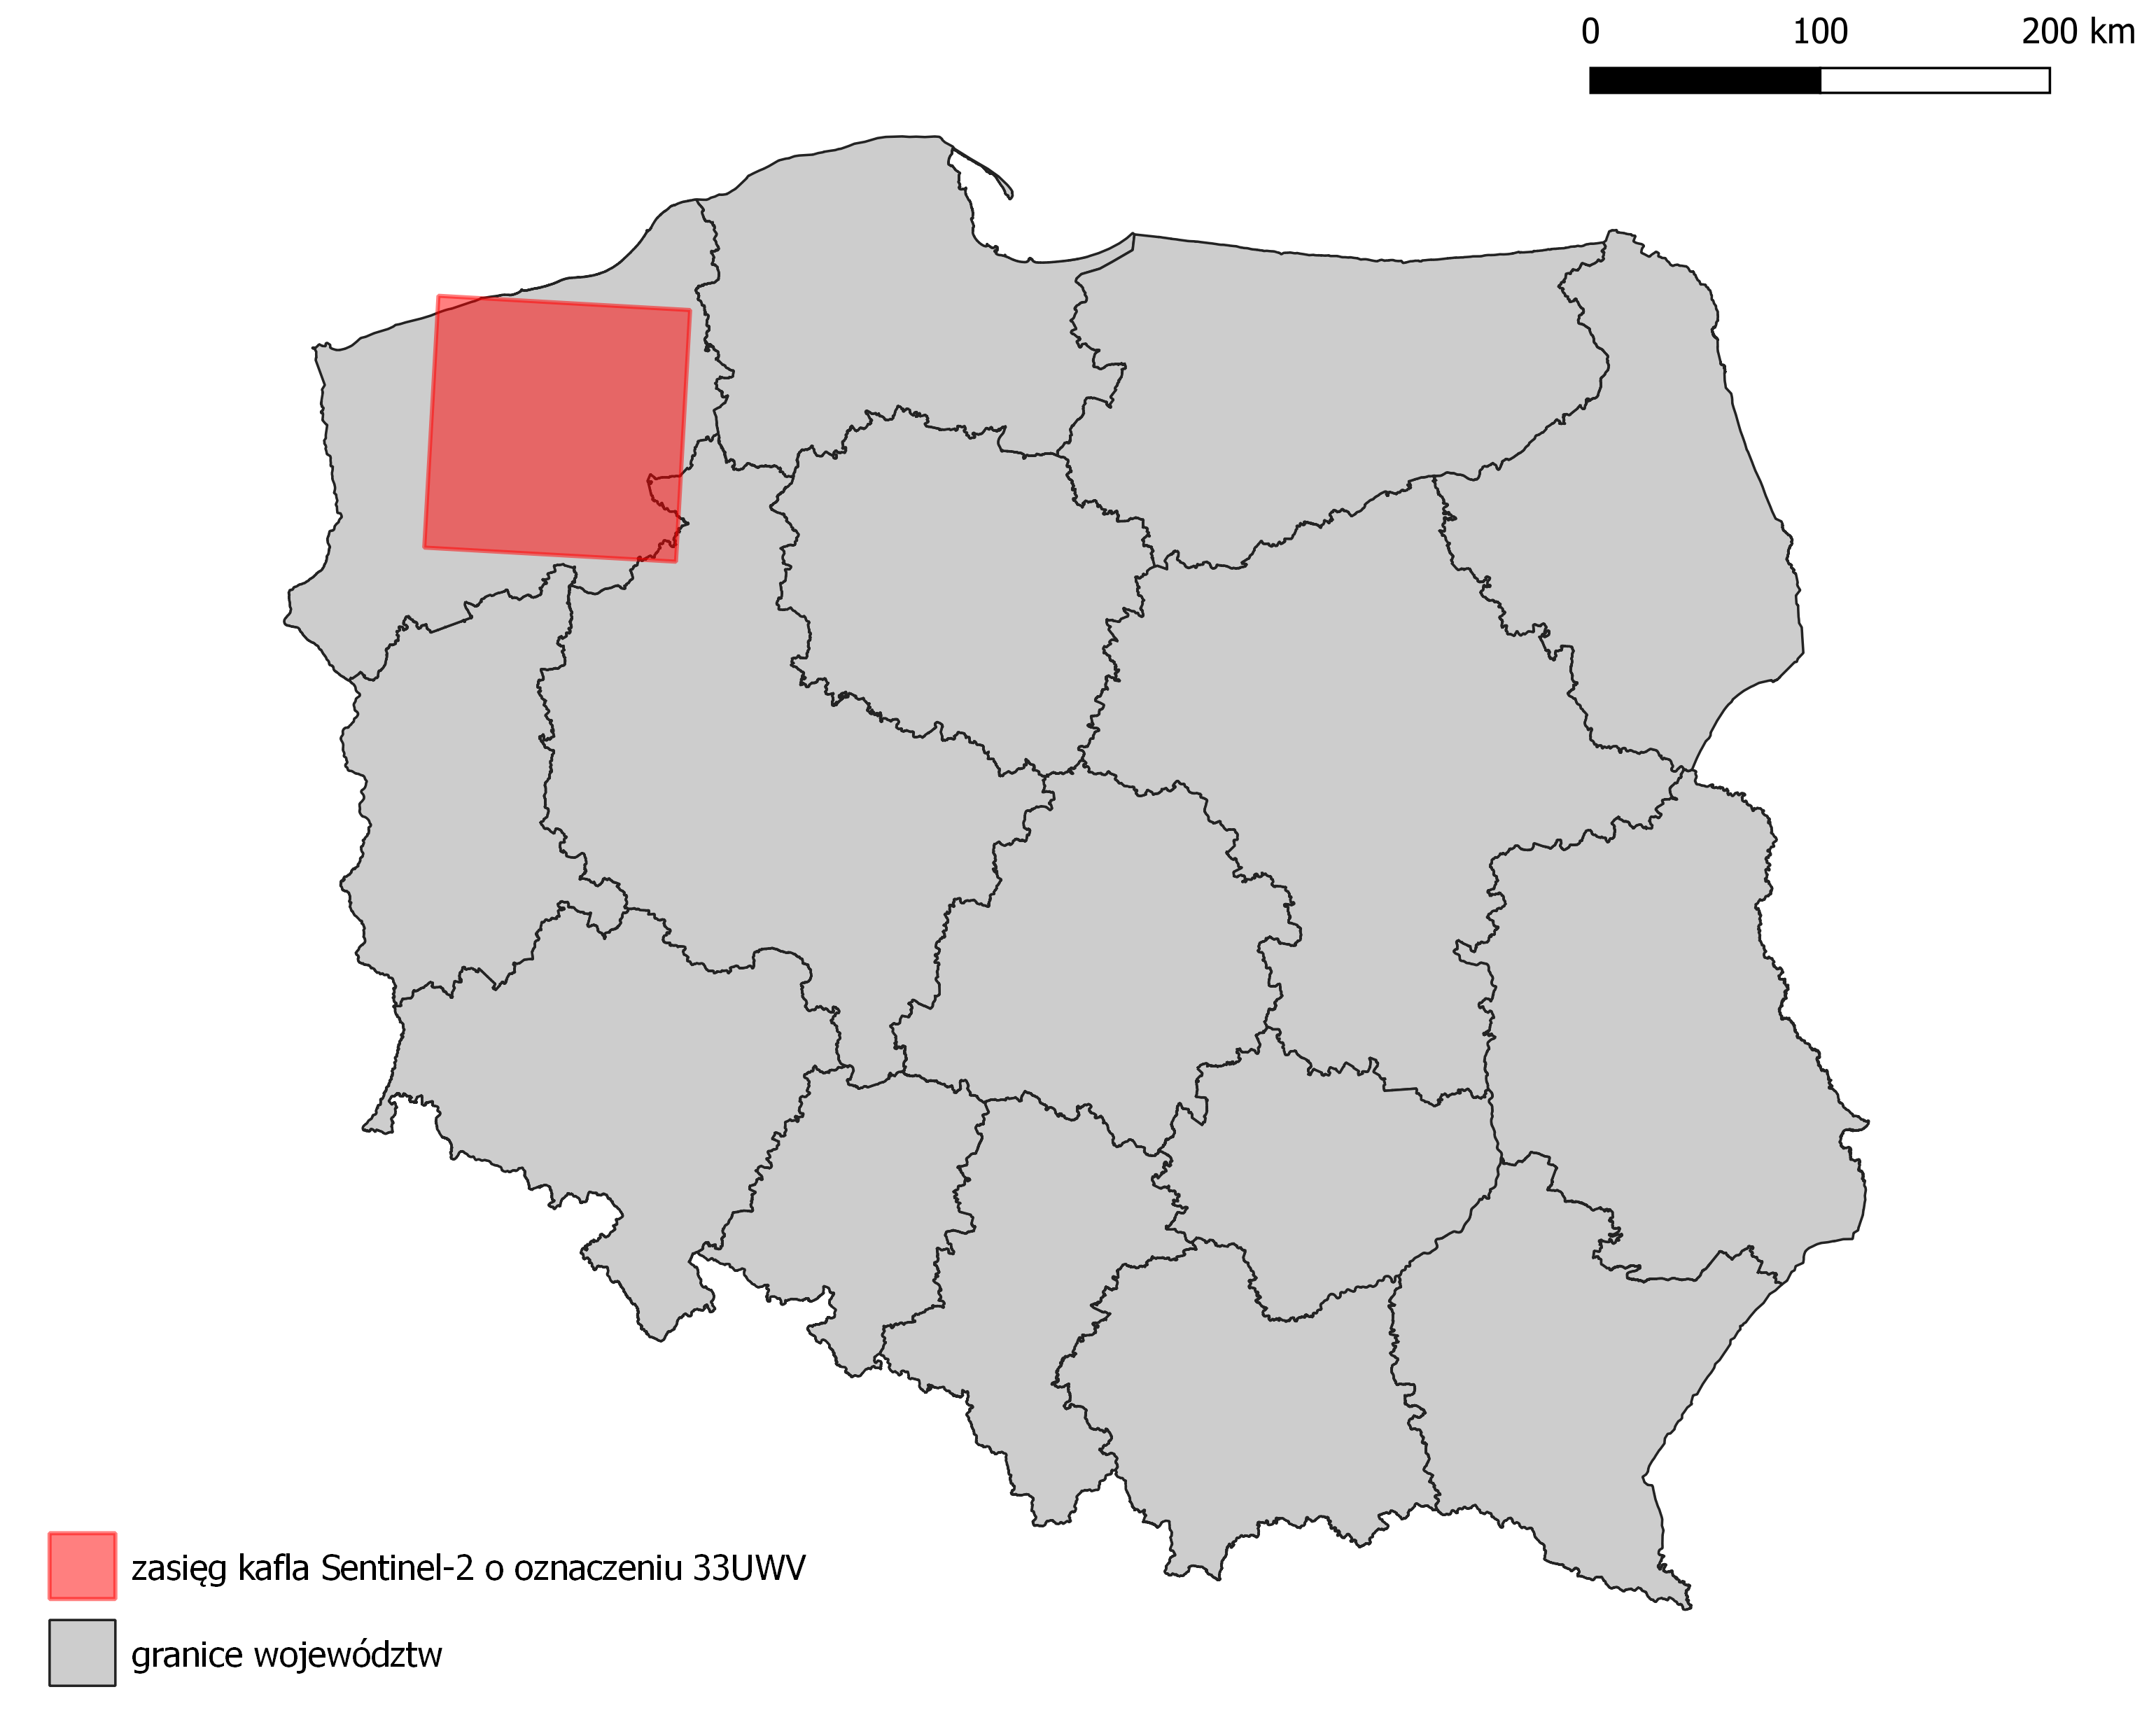
\includegraphics[width=1\textwidth,height=\textheight]{figures/sen2_extent.png}

}

\caption{\label{fig-rycina-area}Obszar badań (zaznaczony kolorem
czerwonym) na tle województw w Polsce}

\end{figure}

\hypertarget{sec-pv}{%
\section{Lokalizacje farm fotowoltaicznych}\label{sec-pv}}

Jednym z zastosowań mozaik obrazów satelitarnych jest tworzenie zestawów
danych referencyjnych poprzez interpretację wizualną, np. w celu
walidacji wyników klasyfikacji produktów pokrycia terenu
\autocite{lesiv_2018_sat_imagery_mosaics}. Do lokalizacji oraz
digitalizacji istniejących farm fotowoltaicznych wykorzystano
ortofotomapę udostępnianą przez Główny Urząd Geodezji i Kartografii
(GUGiK) oraz mozaiki zdjęć satelitarnych dostarczane przez podmioty
komercyjne. W celu stworzenia zbioru danych testowych i treningowych
użyto ortomozaik Google Satellite, Bing Aerial oraz Planet Basemaps
\autocite{planet}, udostępnianych w formie usług sieciowych (WMS, WMTS,
XYZ Tiles). Mozaiki te są tworzone na podstawie komercyjnych zdjęć
satelitarnych wykonywanych przez podmioty takie jak Maxar Technologies,
Airbus czy Planet Labs.

\begin{figure}[H]

{\centering 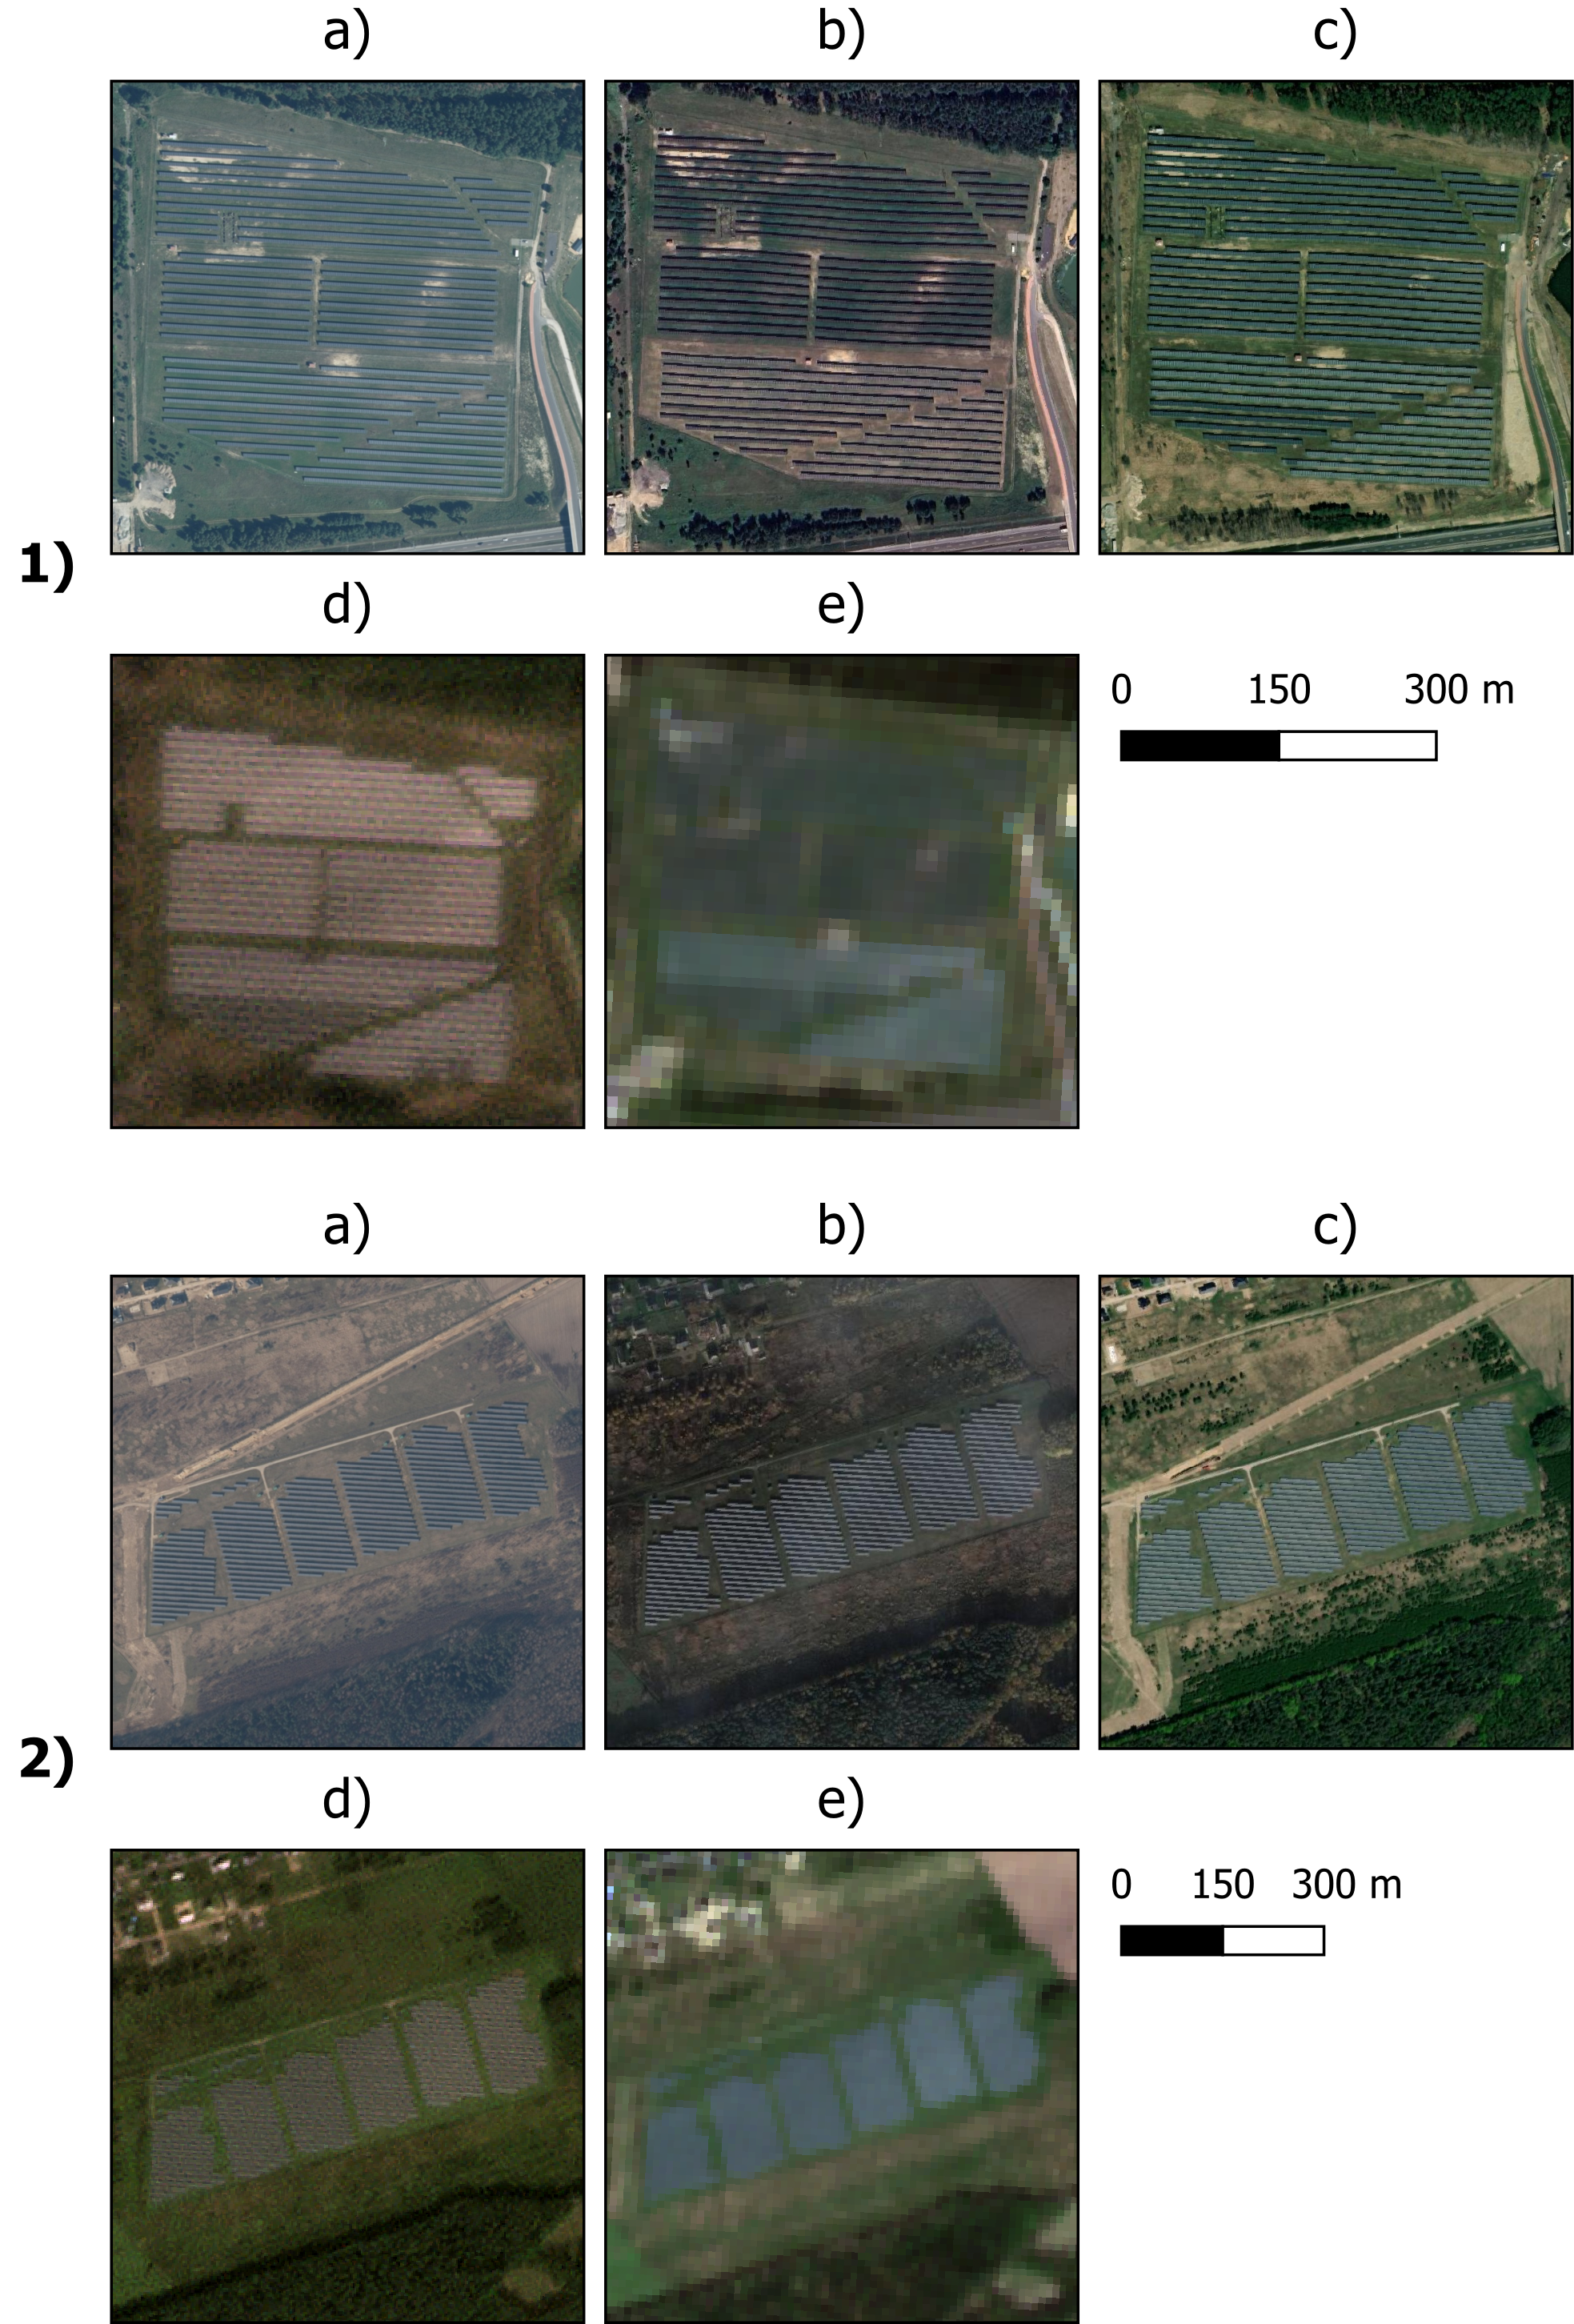
\includegraphics[width=1\textwidth,height=\textheight]{figures/pv.png}

}

\caption{\label{fig-rycina-pv}Porównanie wyglądu farm fotowoltaicznych w
Kulicach k. Nowogardu (1) i Wałczu (2) na ortofotomapie udostępnianej
przez GUGiK (a), Google Satellite (b), Bing Aerial (c), Planet Basemaps
(d) oraz w kompozycji RGB Sentinel-2 (e)}

\end{figure}

Większość ortofotomap dostarczanych przez GUGiK jest zrealizowana w
standardzie 25 x 25 cm, jednakże na obszarach miejskich charakteryzują
się one rozdzielczością przestrzenną wynoszącą 10 cm lub nawet wyższą
\autocite{ortofotomapa}. Rozdzielczość przestrzenna wykorzystanych
mozaik obrazów satelitarnych (oprócz Planet Basemaps) jest wyższa niż 1
m, na przykład mozaika Bing Aerial dostarczana przez firmę Microsoft
cechuje się rozmiarem komórki od 30 do 60 cm \autocite{bing_aerial}.
Często jednak nie jest możliwie ustalenie dat wykonania zdjęć
satelitarnych, które posłużyły do stworzenia konkretnej mozaiki
zobrazowań satelitarnych \autocite{lesiv_2018_sat_imagery_mosaics}.
Mozaika tworzona przez Planet na podstawie zdjęć satelitarnych
wykonywanych przez konstelację satelitów PlanetScope charakteryzuje się
niższą rozdzielczością przestrzenną (4,77 m na równiku), jednak w
porównaniu do pozostałych wymienionych produktów jest tworzona z
miesięczną oraz kwartalną częstotliwością
\autocite{planet_2019_basemaps}. Pozwala to, pomimo niższej
rozdzielczości przestrzennej, na stworzenie zbioru danych referencyjnych
dla konkretnego zakresu czasu. Mozaiki Planet Basemaps \autocite{planet}
są tworzone na podstawie najlepszych obrazów z katalogu Planet w
określonym przedziale czasowym, co umożliwia generowanie
wysokorozdzielczych mozaik, które są dokładne radiometrycznie i
przestrzennie, a także charakteryzują się zminimalizowanym wpływem
czynników atmosferycznych \autocite{planet_2019_basemaps}.

Na podstawie wyżej wymienionych danych dokonano digitalizacji farm
fotowoltaicznych na obszarze badania w celu stworzenia zestawu danych
referencyjnych. Digitalizacja polega na tworzeniu obiektów wektorowych,
takich jak punkty, linie czy poligony, poprzez rysownie figur
geometrycznych uwzględniając ich współrzędne geograficzne na podstawie
obrazów satelitarnych czy zeskanowanych map papierowych. Do tego celu
wykorzystano narzędzia digitalizacji z oprogramowania QGIS
\autocite{qgis}, które umożliwiają rysowanie kształtów i edycję danych
wektorowych.

Na podstawie ortofotomapy oraz mozaik satelitarnych zdigitalizowane
zostały wszystkie znalezione farmy fotowoltaiczne na obszarze kafla
33UWV Sentinel-2, istniejące w czasie wykonywania wykorzystanych
zobrazowań (8 maja 2023 roku, sekcja \ref{sec-satellite-imagery}). Użyte
do digitalizacji dane pochodzą z różnych okresów, co spowodowało
sytuacje, gdzie farmy obecne na najbardziej aktualnej mapie podkładowej
(Planet Basemaps) nie występowały na mozaikach o wyższej rozdzielczości
przestrzennej (ortofotomapa, Google Satellite, Bing Aerial). Podczas
digitalizacji przyjęto, że granice farm fotowoltaicznych lub ich
segmentów będą ustalane na podstawie mapy podkładowej o najwyższej
rozdzielczości, na której dana farma fotowoltaiczna występuje.

\hypertarget{tbl-tabela-digitizing-results}{}
\begin{table}
\caption{\label{tbl-tabela-digitizing-results}Statystki zdigitalizowanych farm fotowoltaicznych na obszarze kafla
Sentinel-2 o~oznaczeniu 33UWV }\tabularnewline

\centering
\begin{tabular}{lr}
\toprule
Liczba zdigitalizowanych farm PV lub ich segmentów & 226\\
Suma powierzchni farm fotowoltaicznych [ha] & 346.47\\
Minimalna powierzchnia farmy PV lub jej segmentu & 0.01\\
Średnia powierzchnia farmy PV lub jej segmentu [ha] & 1.53\\
Maksymalna powierzchnia farmy PV lub jej segmentu [ha] & 24.89\\
\bottomrule
\end{tabular}
\end{table}

Podstawowe statystki zdigitalizowanych obiektów przedstawia tabela
\ref{tbl-tabela-digitizing-results}, a lokalizacje oznaczonych farm
fotowoltaicznych lub ich segmentów przedstawia rycina
\ref{fig-rycina-spatial-distribution-pv}. Zauważyć można duże
zróżnicowanie w powierzchni farm fotowoltaicznych lub ich segmentów, od
małych instalacji o powierzchni 0,01 ha do znacznie większych
konstrukcji o powierzchni prawie 25 ha. Rozmieszczenie farm
fotowoltaicznych na obszarze kafla 33UWV Sentinel-2 skupia się głównie w
zachodniej i południowej części badanego obszaru (rycina
\ref{fig-rycina-spatial-distribution-pv}).

\begin{figure}[H]

{\centering 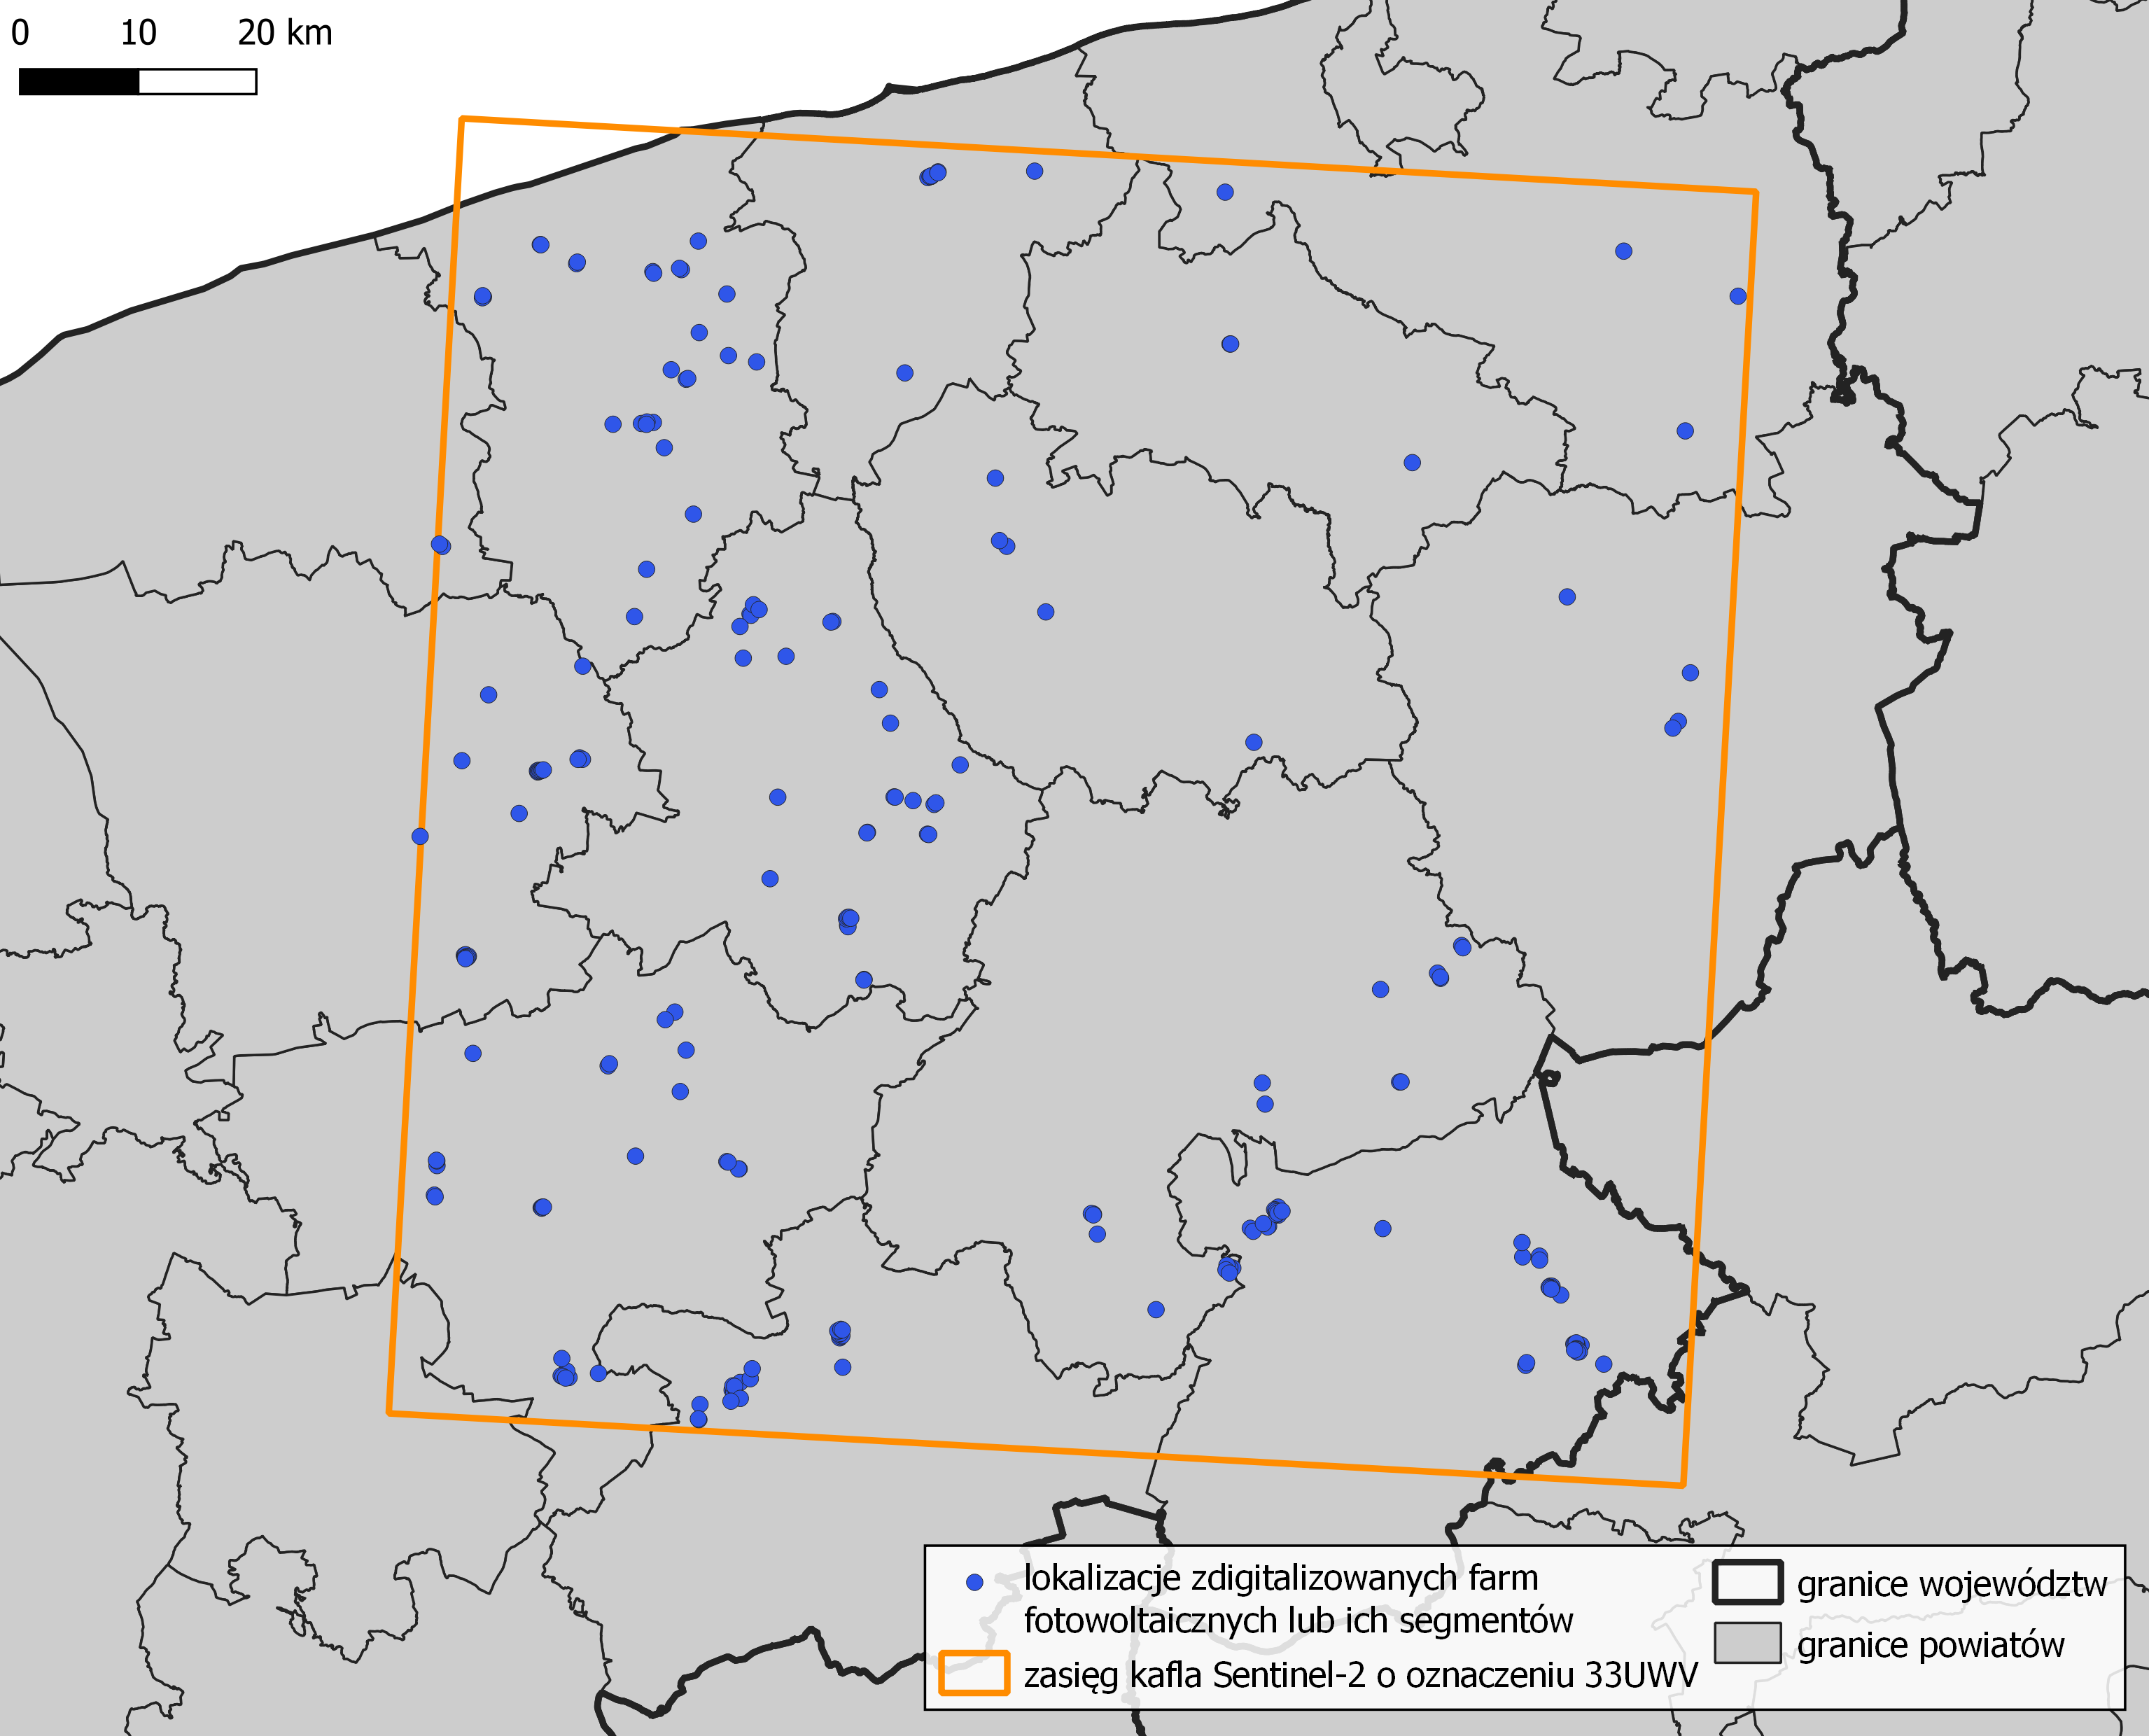
\includegraphics[width=0.76\textwidth,height=\textheight]{figures/farmy2.png}

}

\caption{\label{fig-rycina-spatial-distribution-pv}Rozmieszczenie
zdigitalizowanych farm fotowoltaicznych lub ich segmentów}

\end{figure}

\hypertarget{sec-satellite-imagery}{%
\section{Zdjęcia satelitarne}\label{sec-satellite-imagery}}

\hypertarget{sec-sentinel1}{%
\subsection{Sentinel-1}\label{sec-sentinel1}}

Misja Sentinel-1 to wspólna inicjatywa Komisji Europejskiej i
Europejskiej Agencji Kosmicznej w ramach programu Copernicus, mająca na
celu dostarczanie danych radarowych obejmujących powierzchnię Ziemi, w
tym lądów, europejskich stref przybrzeżnych, tras żeglugowych, stref
lodu morskiego, mórz i oceanów
\autocite{hejmanowska_2020_dane,sentinel1_mission_objectives}. Misja
odpowiada na potrzeby monitorowania obszarów morskich i lądowych, w tym
przemieszczania kry lodowej, transportu morskiego, deformacji i
przemieszczeń terenu, a także obserwacji zmian klimatu i klęsk
żywiołowych
\autocite{hejmanowska_2020_dane,sentinel1_mission_objectives}.

Sentinel-1 posiada pojedynczy radar z syntetyzowaną aperturą (ang.
\emph{Synthetic Aperture Radar}, SAR), który działa na jednej
częstotliwości środkowej 5,405 GHz, odpowiadającej długości fali 5,6 cm
\autocite{sentinel1_lulc,sentinel1_instrument_payload}. Częstotliwość
radaru Sentinel-1, mieszcząca się w pasmie C (od 4 do 8 GHz),
determinuje jego zdolność do penetracji jedynie górnych warstw koron
drzew, roślinności oraz gleby \autocite{sentinel_1_user_guide}. Radar
jest najczęściej wykorzystywany w trybie podwójnej polaryzacji, emitując
fale pionowe i mierząc zarówno fale pionowe (ang. \emph{vertical}), jak
i poziome (ang. \emph{horizontal}) po ich powrocie do czujnika, dzięki
czemu otrzymujemy dane o intensywności rozproszenia wstecznego VV i VH
\autocite{sentinel1_lulc}. Radar z syntetyzowaną aperturą umożliwia
prowadzenie obserwacji zarówno w nocy, jak i w dzień, niezależnie od
warunków pogodowych, przez co czas rewizyty konstelacji dwóch satelitów
dla obszaru Polski wynosi około 2 dni
\autocite{attema_2008_s1,sentinel1_revisit}. W grudniu 2021 roku w
satelicie Sentinel-1B wystąpiła awaria układu zasilania elektroniki
radaru, uniemożliwiająca dalsze dostarczanie danych radarowych
\autocite{sentinel_1b}. W wyniku awarii satelita Sentinel-1B został
wyłączony z użytku, a wystrzelenie platformy Sentinel-1C zaplanowano na
marzec 2024 roku \autocite{sentinel_1b,sentinel1_eoportal}.

\begin{figure}[t]

{\centering 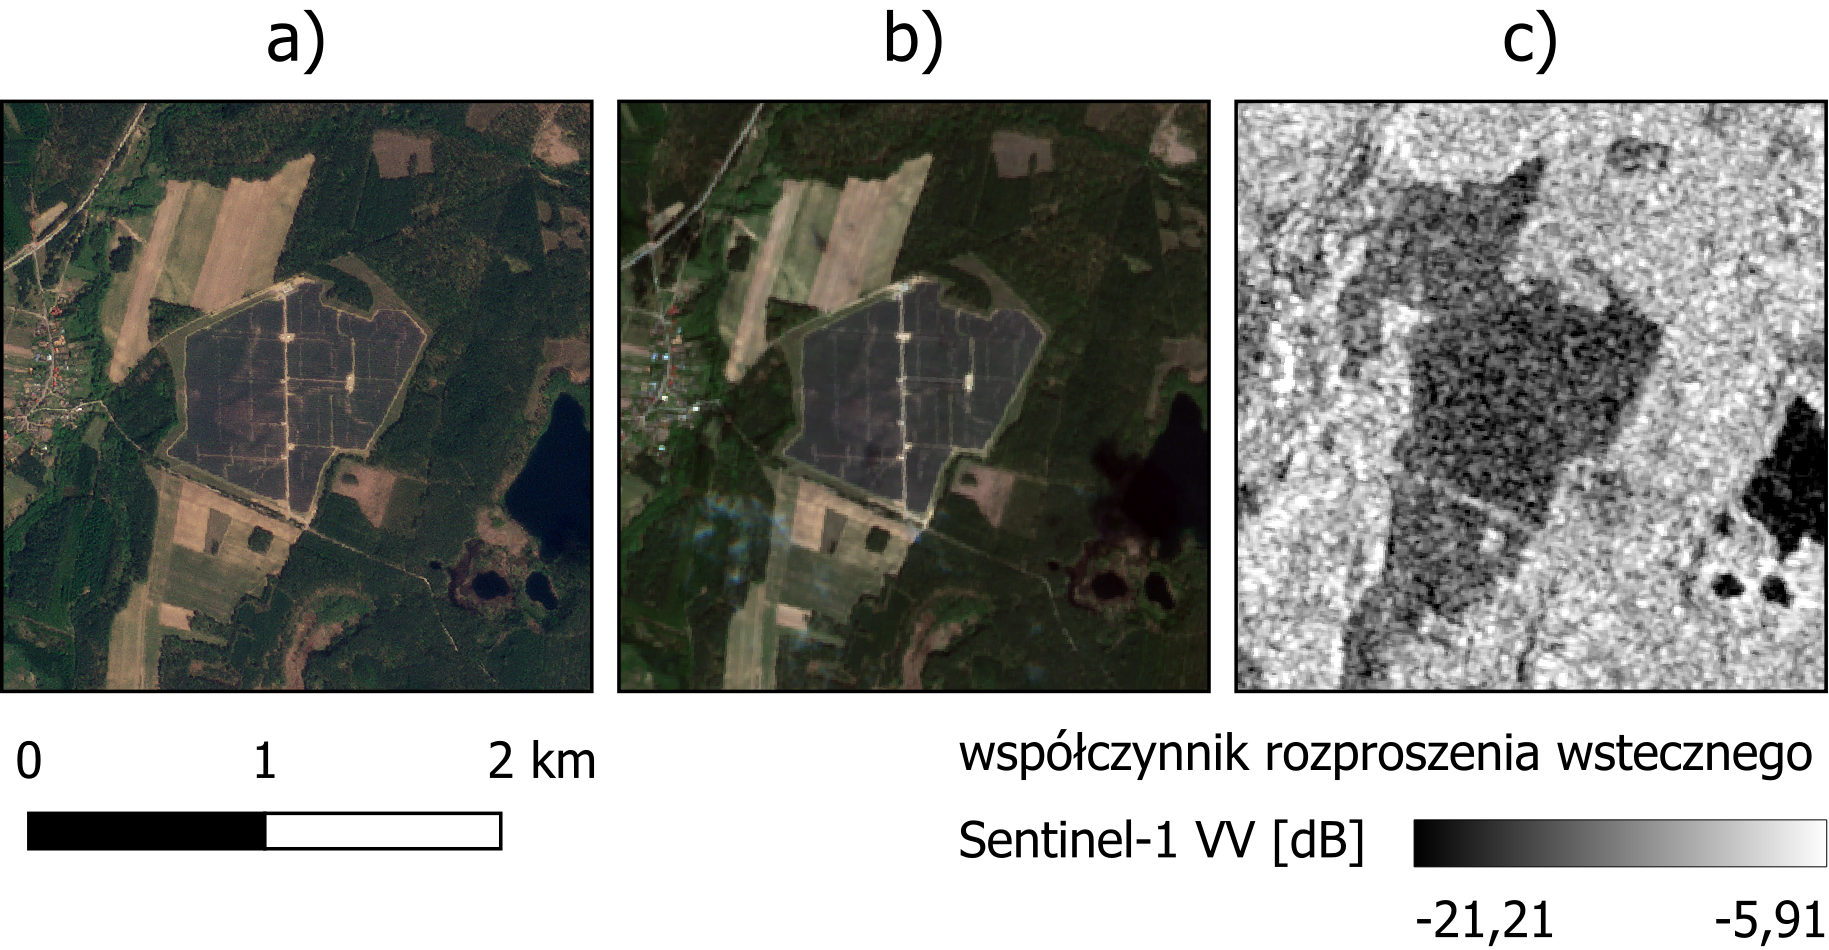
\includegraphics[width=1\textwidth,height=\textheight]{figures/pv_sentinel1.png}

}

\caption{\label{fig-rycina-pv-sentinel1}Farma fotowoltaiczna na
wysokorozdzielczym obrazie satelitarnym PlanetScope (a), kompozycji RGB
Sentinel-2 (b) oraz obrazie rozproszenia wstecznego w polaryzacji VV
Sentinel‑1~(c)}

\end{figure}

Dane radarowe Sentinel-1 są dostępne na trzech poziomach przetworzenia.
Dane poziomu 0 to surowe, nieobrazowe dane, z których generowane są
produkty wyższych poziomów przetworzenia. Poziom 1 obejmuje produkty
Single Look Complex (SLC) oraz Ground Range Detected (GRD) przeznaczone
do monitorowania Ziemi, klasyfikacji pokrycia terenu oraz aplikacji
interferometrycznych \footnote{Interferometria radarowa (ang.
  \emph{Interferometric Synthetic Aperture Radar}, InSAR) to technika
  umożliwiająca generowanie cyfrowych modeli wysokościowych (ang.
  \emph{digital elevation model}, DEM) oraz pomiary deformacji terenu na
  podstawie informacji o fazie sygnału
  \autocite{hanssen_2001_insar,hejmanowska_2020_dane}.}
\autocite{hejmanowska_2020_dane}. Produkty SLC to obrazy SAR w geometrii
ukośnej, posiadające informację o wartości amplitudy i fazie sygnału, co
czyni je odpowiednimi do interferometrii radarowej
\autocite{hejmanowska_2020_dane}. Produkty GRD są rezultatem
przepróbkowania obrazów SLC do jednolitej rozdzielczości przestrzennej
(10 × 10 m) i rzutowania na powierzchnię elipsoidy odniesienia
\autocite{hejmanowska_2020_dane}. Przy konwersji SLC do GRD tracimy
informację fazową sygnału, co wyklucza zastosowanie produktów GRD w
interferometrii radarowej \autocite{sentinel1_products}. Produkty GRD
nie posiadają cech ortofotomapy i wymagają dodatkowego przepróbkowania z
użyciem cyfrowego modelu wysokości przed wykorzystaniem w systemach GIS
\autocite{hejmanowska_2020_dane}. Produkty oceaniczne poziomu drugiego
(Level-2 Ocean (OCN)) służą natomiast do zastosowań związanych z
pomiarem wiatrów, fal i prądów morskich \autocite{sentinel1_ocn}.
Produkty przeznaczone dla użytkowników końcowych to produkty pierwszego
i drugiego poziomu przetworzenia.

Dane Sentinel-1 rejestrowane są w czterech trybach: Stripmap (SM) -
używany do obrazowania małych wysp i na potrzeby zarządzania
kryzysowego, Interferometric Wide Swath (IW) - podstawowy tryb
obrazowania dla obszarów lądowych, Extra-Wide Swath (EW) - tryb do
monitorowania stref polarnych i niektórych obszarów morskich oraz Wave
(WV) - tryb obrazowania oceanów
\autocite{hejmanowska_2020_dane,sentinel1_instrument_payload,sentinel1_stripmap}.
Charakterystykę konkretnych trybów akwizycji radaru Sentinel-1
przedstawia tabela \ref{tbl-tabela-sentinel1}
\autocite{sentinel1_resolution_swath}.

\hypertarget{tbl-tabela-sentinel1}{}
\begin{table}
\caption{\label{tbl-tabela-sentinel1}Tryby radaru Sentinel-1 (ESA,
\href{https://sentinels.copernicus.eu/web/sentinel/missions/sentinel-1/instrument-payload/resolution-swath}{2023}).
Pogrubiony wiersz wskazuje tryb wykorzystany w niniejszym badaniu. }\tabularnewline

\centering
\begin{tabular}{>{\centering\arraybackslash}p{3cm}>{\centering\arraybackslash}p{1.8cm}>{\centering\arraybackslash}p{2.4cm}>{\centering\arraybackslash}p{2.8cm}>{\centering\arraybackslash}p{2cm}}
\toprule
Tryb & Kąt padania wiązki [°] & Rozdzielczość przestrzenna [m] & Szerokość rejestrowanego pasa [km] & Polaryzacje (H=pozioma, V=pionowa)\\
\midrule
Stripmap & 20 - 45 & 5 x 5 & 80 & HH+HV, VH+VV, HH, VV\\
\addlinespace
\textbf{Interferometric Wide Swath} & \textbf{29 - 46} & \textbf{5 x 20} & \textbf{250} & \textbf{HH+HV, VH+VV, HH, VV}\\
\addlinespace
Extra Wide Swath & 19 - 47 & 20 x 40 & 400 & HH+HV, VH+VV, HH, VV\\
\addlinespace
Wave & 22 - 35   35 - 38 & 5 x 5 & 20 x 20 & HH, VV\\
\bottomrule
\end{tabular}
\end{table}

W pracy wykorzystano dwie polaryzacje (VV i VH) pochodzące z produktów
Ground Range Detected, zarejestrowanych w trybie Interferometric Wide
Swath przez platformę Sentinel-1A w dniu 8 maja 2023 roku. Podczas
rejestracji danych platforma znajdowała się na orbicie wznoszącej (ang.
\emph{ascending orbit}), co oznacza, że satelita przemieszczał się z
południa w kierunku bieguna północnego. Użyty zestaw danych został
utworzony poprzez połączenie dwóch sąsiednich produktów Sentinel-1 GRD,
a następnie ograniczenie obszaru analizy do kafla Sentinel-2 o
oznaczeniu 33UWV.

\hypertarget{sec-sentinel2}{%
\subsection{Senitnel-2}\label{sec-sentinel2}}

Misja Sentinel-2 stanowi inicjatywę Komisji Europejskiej, która jest
operacyjnie prowadzona przez Europejską Agencję Kosmiczną w ramach
programu Copernicus. Celem tej misji jest dostarczanie obrazów
satelitarnych, obejmujących trzynaście zakresów spektralnych o różnych
rozdzielczościach przestrzennych: 10, 20 lub 60 metrów, zależnie od
rejestrowanego kanału. Czas rewizyty konstelacji dwóch satelitów wzrasta
z 5 dni nad równikiem do 2-3 dni na średnich szerokościach
geograficznych, obejmujących również obszar Polski
\autocite{hejmanowska_2020_dane,sentinel_2_guide}.

\hypertarget{tbl-tabela-sentinel2}{}
\begin{table}
\caption{\label{tbl-tabela-sentinel2}Kanały spektralne satelitów Sentinel-2 (ESA,
\href{https://sentinels.copernicus.eu/web/sentinel/user-guides/sentinel-2-msi/resolutions/spectral}{2023}).
Pogrubione wiersze wskazują kanały wykorzystane w niniejszym badaniu. }\tabularnewline

\centering
\begin{tabular}{>{\centering\arraybackslash}p{1.5cm}>{\centering\arraybackslash}p{4cm}>{\centering\arraybackslash}p{2cm}>{\centering\arraybackslash}p{2cm}>{\centering\arraybackslash}p{2.4cm}}
\toprule
Kanał & Nazwa kanału & Centralna długość fali [nm] & Zakres spektralny [nm] & Rozdzielczość przestrzenna [m]\\
\midrule
B01 & Coastal Aerosol & 443 & 433–453 & 60\\
\textbf{B02} & \textbf{Blue} & \textbf{493} & \textbf{458–523} & \textbf{10}\\
\textbf{B03} & \textbf{Green} & \textbf{560} & \textbf{543–578} & \textbf{10}\\
\textbf{B04} & \textbf{Red} & \textbf{665} & \textbf{650–680} & \textbf{10}\\
\textbf{B05} & \textbf{Vegetation RedEdge} & \textbf{704} & \textbf{698–713} & \textbf{20}\\
\textbf{B06} & \textbf{Vegetation RedEdge} & \textbf{740} & \textbf{733–748} & \textbf{20}\\
\textbf{B07} & \textbf{Vegetation RedEdge} & \textbf{783} & \textbf{773–793} & \textbf{20}\\
\textbf{B08} & \textbf{NIR} & \textbf{833} & \textbf{785–900} & \textbf{10}\\
\textbf{B8A} & \textbf{NIR} & \textbf{865} & \textbf{855–875} & \textbf{20}\\
B09 & Water Vapour & 945 & 935–955 & 60\\
B10 & Cirrus & 1374 & 1360–1390 & 60\\
\textbf{B11} & \textbf{SWIR} & \textbf{1610} & \textbf{1565–1655} & \textbf{20}\\
\textbf{B12} & \textbf{SWIR} & \textbf{2190} & \textbf{2100–2280} & \textbf{20}\\
\bottomrule
\end{tabular}
\end{table}

Dane pozyskiwane przez satelity Sentinel-2 są dostępne na różnych
poziomach przetworzenia, lecz najczęściej używane przy tworzeniu map
pokrycia terenu i użytkowania ziemi (ang. \emph{Land Use/Land Cover},
LULC) są produkty 1C (współczynnik odbicia na poziomie górnej części
atmosfery; ang. \emph{Top-of-Atmospheric reflectance}, TOA) oraz 2A
(współczynnik odbicia na powierzchni Ziemi; ang.
\emph{Bottom-of-Atmospheric reflectance}, BOA)
\autocite{phiri_2020_sentinel2}.

Produkty poziomu 1C to dane poddane korekcjom radiometrycznym i
geometrycznym, prezentowane jako sceny (ang. \emph{tile},
\emph{granule}) o zasięgu 100 x 100 km w projekcji UTM/WGS84
\autocite{esa_2015_sentinel2handbook}. Skuteczne wykorzystanie tych
danych w zastosowaniach związanych z terenami lądowymi wymaga
precyzyjnej korekcji zdjęć satelitarnych pod kątem efektów
atmosferycznych \autocite{main-knorn_2017_Sen2Cor}. Produkty poziomu 2A
powstają poprzez zastosowanie dodatkowej korekcji atmosferycznej dla
danych poziomu 1C za pomocą procesora korekcji atmosferycznej Sen2Cor
\autocite{main-knorn_2017_Sen2Cor}.

Dane wykorzystane w analizie pochodzą z dnia 8 maja 2023 roku i zostały
dostarczone przez satelitę Sentinel-2B. Obszar analizy obejmuje kafel
(ang. \emph{tile}) o oznaczeniu 33UWV, dla którego współczynnik
zachmurzenia w tym dniu wynosił 0,7\%. Użyte zostały dane na poziomie
przetworzenia L2A. Z dostępnych kanałów spektralnych (tabela
\ref{tbl-tabela-sentinel2}) wykorzystano 10 zakresów, ponieważ pasma
rejestrowane w rozdzielczości 60 metrów są przeznaczone głównie do
korekcji atmosferycznych i detekcji chmur. Kanał 1 (443 nm) służy do
korekcji wpływu aerozoli, kanał 9 (945 nm) do korekcji wpływu pary
wodnej, a kanał 10 (1374 nm) do wykrywania chmur typu cirrus
\autocite{drusch_2012_sen2GMES}.

\bookmarksetup{startatroot}

\hypertarget{sec-metody}{%
\chapter{Metody}\label{sec-metody}}

Badanie obejmowało kilka etapów, rozpoczynając od wstępnego
przetwarzania danych satelitarnych, opisanego w sekcjach
\ref{sec-processing-s1} i \ref{sec-processing-s2}. Następnie
przeprowadzono obliczenia produktów pochodnych, takich jak wskaźniki
spektralne oraz tekstury obrazu, opisane odpowiednio w sekcjach
\ref{sec-spectral-indices} i \ref{sec-textures}. Kolejnym krokiem było
połączenie przetworzonych danych źródłowych i ich produktów pochodnych w
kilka wariantów zbiorów danych, stworzonych na potrzeby detekcji farm
fotowoltaicznych. Warianty zbiorów danych przedstawia tabela
\ref{tbl-tabela-datasets}, a przebieg łączenia danych w wielowarstwowe
rastry został opisany w sekcji \ref{sec-processing-data-merging}. Na
podstawie uzyskanych rastrów, zgodnie z sekcją \ref{sec-samples},
utworzono zbiory danych uczących, które zostały wykorzystane do
tworzenia modeli predykcyjnych. W procesie klasyfikacji wykorzystano
metodę lasów losowych (ang. \emph{Random Forest}, RF) zaproponowaną
przez Breimana \autocite*{breiman_2001_rf}, która została dokładniej
przedstawiona w sekcji \ref{sec-random-forest}. Następnie
zoptymalizowano parametry tych modeli, oceniono ich jakość oraz ważność
zmiennych dla każdego z nich, co opisano odpowiednio w sekcjach
\ref{sec-tuning}, \ref{sec-model-quality-assessment} oraz
\ref{sec-variable-importance}. Ostatecznie, przeprowadzono predykcje, a
uzyskane wyniki poddano procesowi przetwarzania końcowego,
przedstawionemu w sekcji \ref{sec-post-processing} \footnote{Wizualną
  reprezentację przebiegu badania można znaleźć pod adresem
  https://github.com/filrat2/wykrywanie-farm-fotowoltaicznych-2024 .}.

Przetwarzanie danych Sentinel-1 GRD zostało przeprowadzane przy użyciu
oprogramowania Sentinel-1 Toolbox (S1TBX) \autocite{s1tbx} i SNAP
\autocite{snap}, udostępnianego przez Europejską Agencję Kosmiczną.
Każdy z kolejnych etapów został wykonany przy użyciu języka R
\autocite{R-base} oraz pakietów rozszerzających funkcjonalności tego
języka. Końcowe wizualizacje zostały stworzone w oprogramowaniu QGIS
\autocite{qgis}. Zarówno oprogramowanie GIS (SNAP, S1TBX, QGIS), jak i
środowisko programistyczne R stanowią oprogramowanie o otwartym kodzie
źródłowym (ang. \emph{open-source software}).

\hypertarget{sec-processing}{%
\section{Przygotowanie danych}\label{sec-processing}}

\hypertarget{sec-processing-s1}{%
\subsection{Sentinel-1}\label{sec-processing-s1}}

Korzystanie z danych radarowych wymaga wcześniejszego przygotowania
danych poprzez proces kalibracji, aby zapewnić poprawne wyniki analizy.
Procesy te mogą różnić się w zależności od konkretnego zastosowania,
mając na celu dostosowanie danych do specyficznych potrzeb. W pracy
wykorzystano schemat przetwarzania danych Sentinel-1 GRD, który
zaproponował \textcite{filipponi_2019_s1_workflow}, obejmujący:

\begin{enumerate}
\def\labelenumi{\arabic{enumi}.}
\item
  aktualizację informacji o położeniu satelity w momencie zobrazowania
  poprzez pobranie dokładnych wektorów stanu orbity dla produktu
  zapewniając precyzyjne informacje o pozycji i prędkości satelity
  podczas akwizycji;
\item
  korekcję szumów termicznych;
\item
  korekcję szumów na granicach obrazów;
\item
  obliczenie współczynnika rozproszenia wstecznego (ang.
  \emph{backscatter coefficient}) sigma0 za pomocą kalibracji
  radiometrycznej;
\item
  korekcję topograficzną (ortorektyfikacja za pomocą Copernicus 30 m
  Global DEM);
\item
  konwersję współczynnika rozproszenia wstecznego na dB za pomocą
  transformacji logarytmicznej
\end{enumerate}

\begin{figure}[t]

{\centering 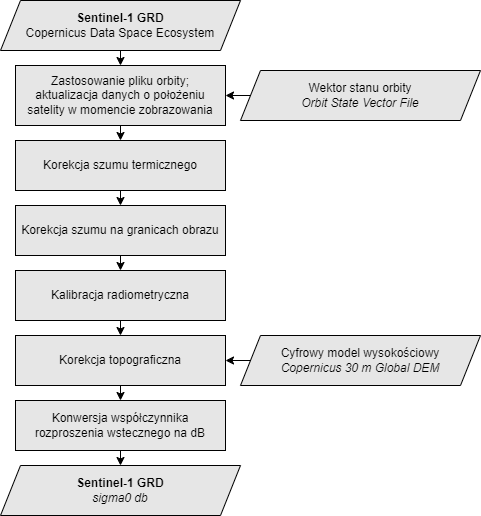
\includegraphics[width=4.6875in,height=\textheight]{figures/sentinel1_workflow.drawio.png}

}

\caption{\label{fig-rycina-s1-workflow}Przebieg wstępnego przetwarzania
danych Sentinel-1 Ground Range Detected (GRD)}

\end{figure}

Podczas przetwarzania danych radarowych pominięto etap filtrowania
plamek (ang. \emph{speckle filtering}), ponieważ ze względu na możliwość
utraty istotnych informacji nie jest to zalecane w kontekście
identyfikacji tekstur obrazu \autocite{filipponi_2019_s1_workflow}.

Dane Sentinel-1 GRD dla obu polaryzacji (VV i VH) przygotowano w sposób
przedstawiony na rycinie \ref{fig-rycina-s1-workflow} przy użyciu
narzędzi dostępnych w ESA Sentinel-1 Toolbox \autocite{s1tbx}, a proces
ten został ułożony w sekwencję operacji przetwarzania za pomocą
narzędzia GraphBuilder w oprogramowaniu SNAP \autocite{snap}. Kolejne
etapy przygotowania danych zostały zrealizowane przy wykorzystaniu
języka R \autocite{R-base} oraz pakietu \emph{terra} \autocite{R-terra}.
Obszar analizy, będący kaflem Sentinel-2 o oznaczeniu 33UWV, znajduje
się na granicy dwóch sąsiednich produktów Sentinel-1 GRD. Na potrzeby
dalszego przetwarzania, sąsiadujące produkty zostały połączone i
odpowiednio ograniczone do obszaru zainteresowania. Na granicy
sąsiednich produktów Sentinel-1 GRD występowała przestrzeń bez danych o
szerokości jednej komórki, co wymagało wypełnienia tego obszaru danymi
przy użyciu funkcji \texttt{focal} z pakietu \emph{terra}
\autocite{R-terra}.

\begin{figure}[t]

{\centering 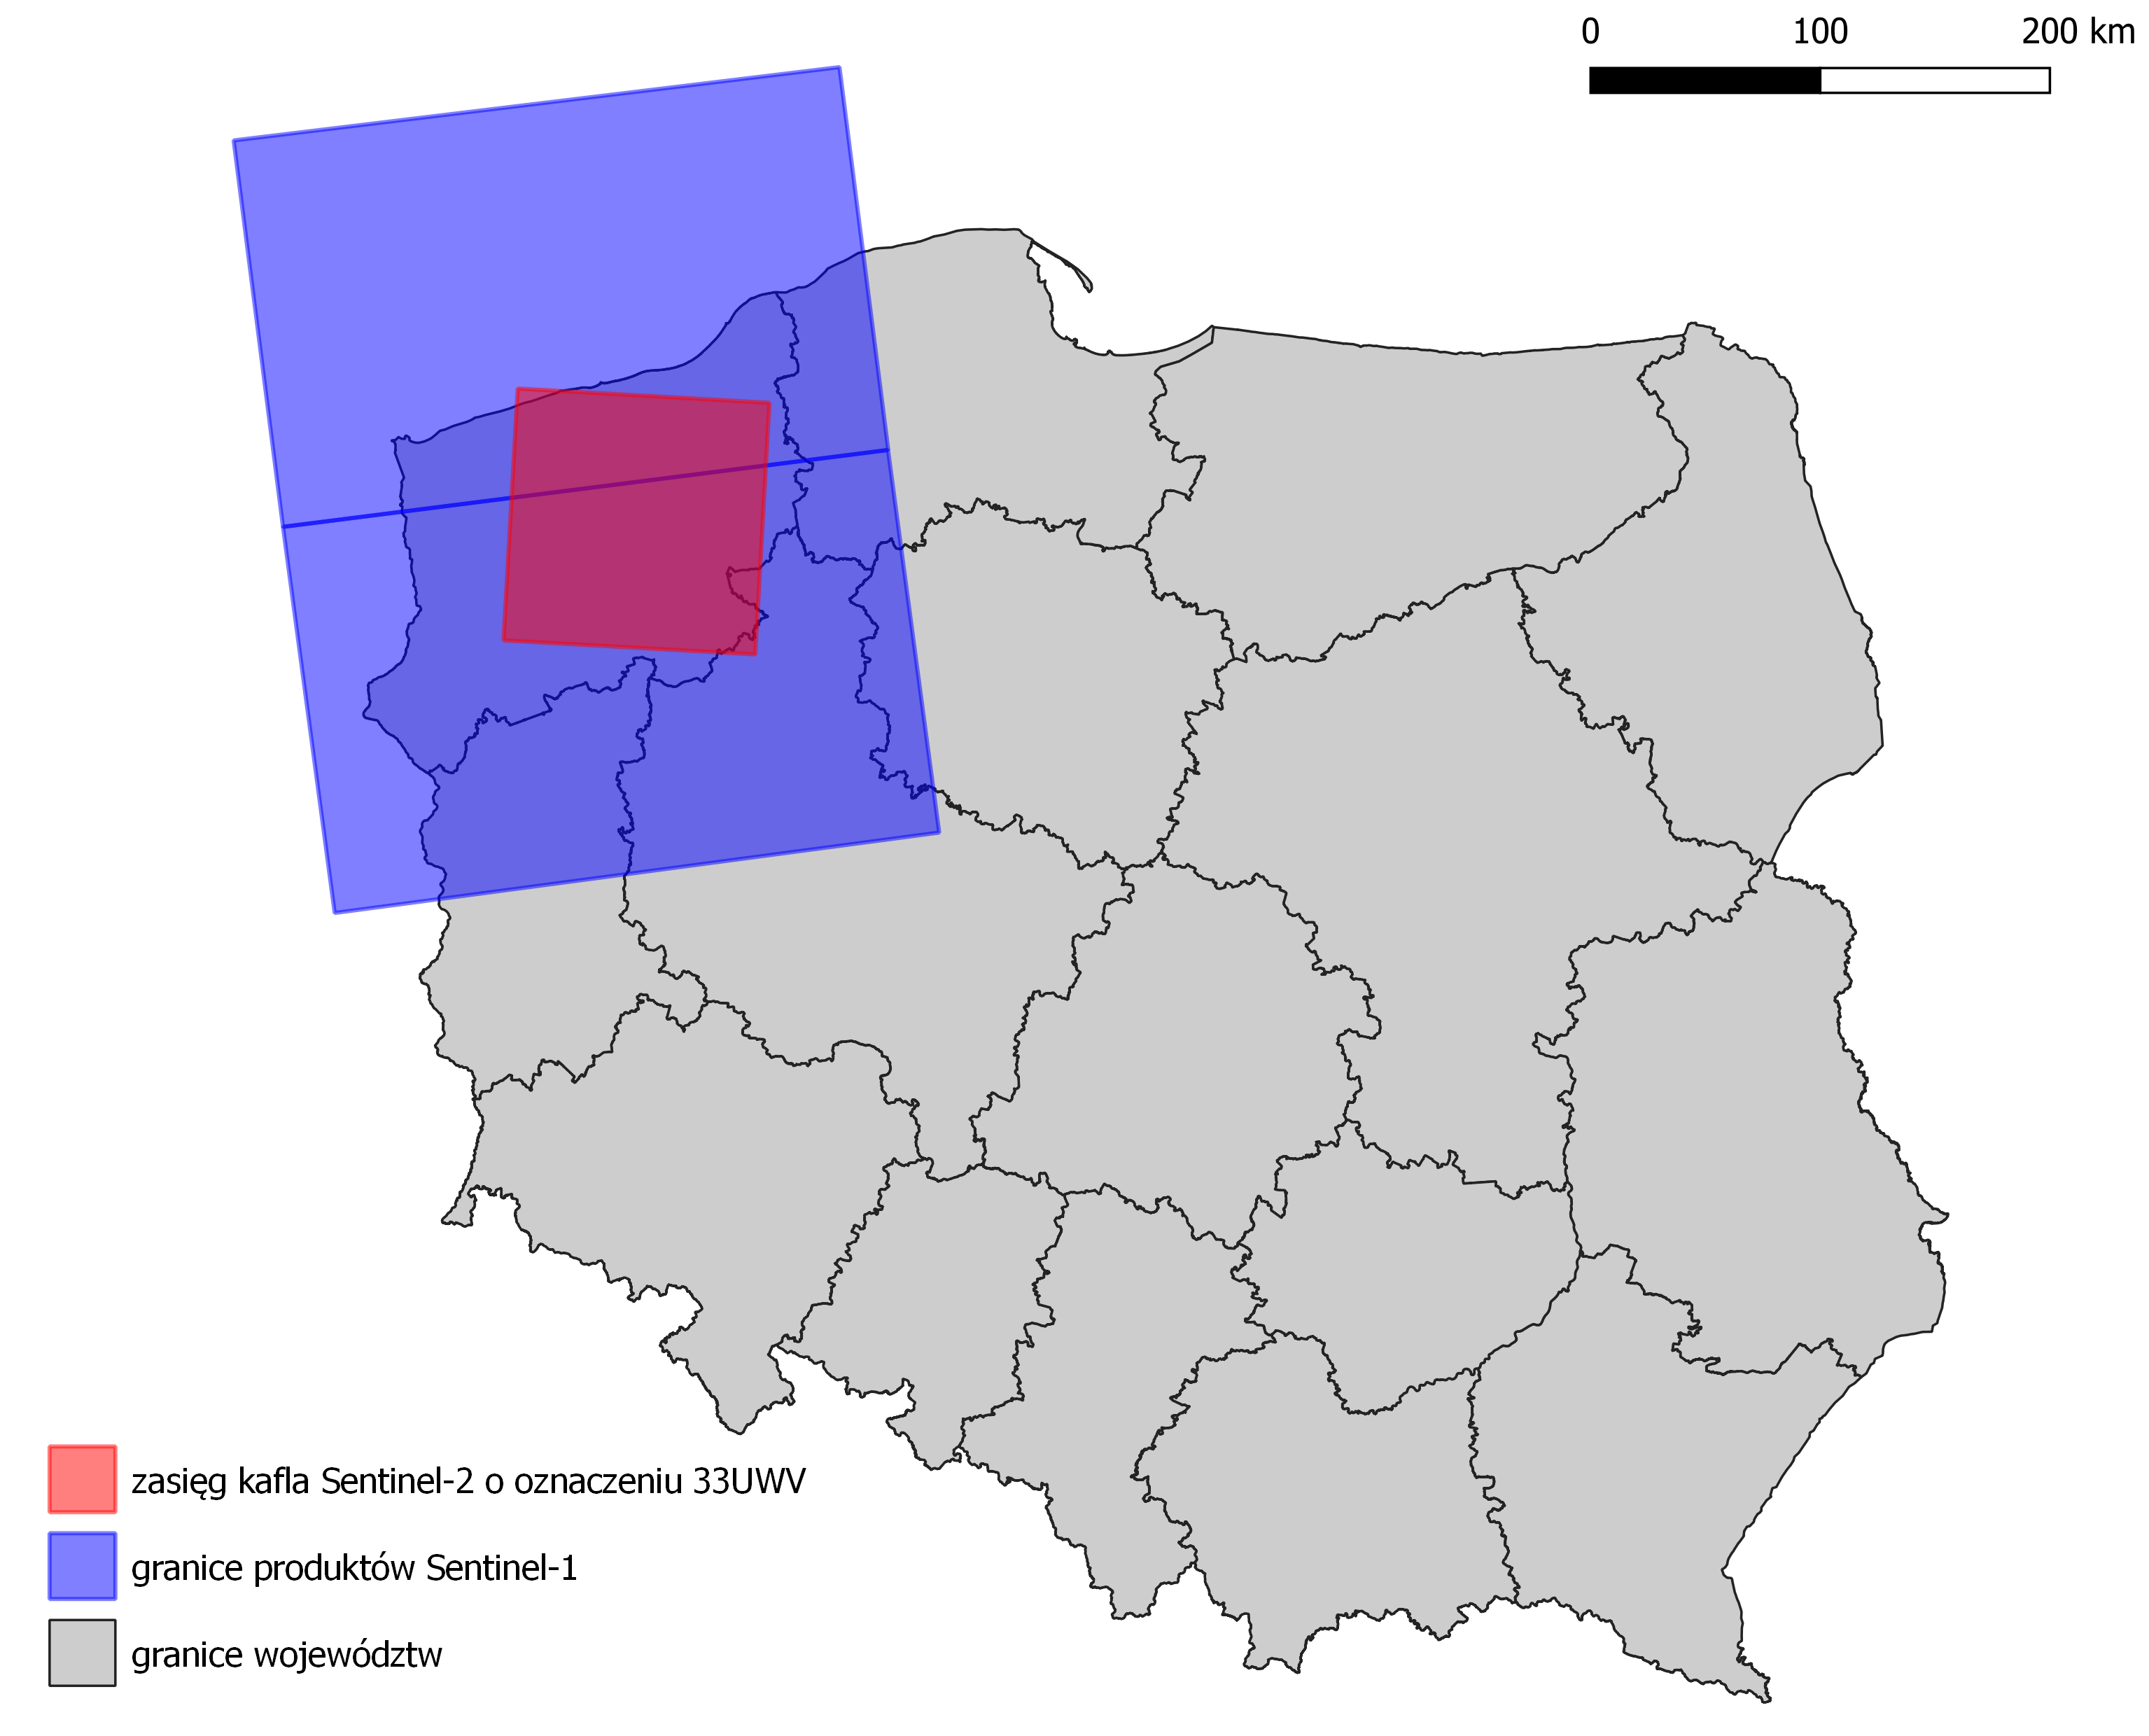
\includegraphics[width=1\textwidth,height=\textheight]{figures/sen1_extents.png}

}

\caption{\label{fig-rycina-s1-extents}Obszar badań (oznaczony kolorem
czerwonym) i zasięg wykorzystanych produktów Sentinel-1 (oznaczonych
kolorem niebieskim) na tle województw w Polsce}

\end{figure}

\hypertarget{sec-processing-s2}{%
\subsection{Sentinel-2}\label{sec-processing-s2}}

Przetwarzanie danych Sentinel-2 polegało na sprowadzeniu kanałów o
rozdzielczości przestrzennej 20 m do rozdzielczości 10 m.
Przepróbkowanie (ang. \emph{resampling}) zostało przeprowadzone przy
pomocy funkcji \texttt{resample} z pakietu \emph{terra}
\autocite{R-terra}, stosując interpolację dwuliniową (ang.
\emph{bilinear interpolation}).

W teledetekcji miarą opisującą wielkość odbicia jest rzeczywisty
współczynnik odbicia, nazywany również reflektancją, którego wartości
mieszczą się w przedziale od 0 do 1 \autocite{hejmanowska_2020_dane}.
Informacje dotyczące odbitego promieniowania w przypadku danych
Sentinel-2 są udostępniane za pomocą współczynnika odbicia, wyrażonego w
zakresie od 0 do 10000, gdzie wartości te reprezentują jasność komórki,
określaną w języku angielskim jako \emph{Digital Number} (DN). Po
standaryzacji wszystkich kanałów Sentinel-2 do wspólnej rozdzielczości,
dokonano przeliczenia wartości kanałów w celu uzyskania rzeczywistego
współczynnika odbicia, poprzez podzielenie wartości DN przez 10000.

\hypertarget{sec-spectral-indices}{%
\subsection{Wskaźniki spektralne}\label{sec-spectral-indices}}

Oprócz surowych współczynników odbicia, w niektórych wariantach
predykcji zastosowano również wskaźniki spektralne (ang. \emph{spectral
indices}), które były wykorzystywane w poprzednich badaniach dotyczących
detekcji farm fotowoltaicznych na podstawie danych teledetekcyjnych
przez Zhanga et al. \autocite*{zhang_2021_texture}, Plakman et al.
\autocite*{plakman_2022_pv}, Wanga et al. \autocite*{wang_2022_pv} i
innych, takie jak:

\begin{itemize}
\item
  znormalizowany różnicowy wskaźnik wegetacji (ang. \emph{Normalized
  Difference Vegetation Index}, NDVI) \autocite{ndvi}, monitorujący
  zawartość biomasy i kondycję roślinności na danym obszarze:

  \[
  NDVI = \frac{NIR - Red}{NIR + Red}
  \]

  , gdzie \(NIR\) -- reflektancja w kanale bliskiej podczerwieni,
  \(Red\) -- reflektancja w kanale czerwonym
\item
  znormalizowany różnicowy wskaźnik obszarów zabudowanych (ang.
  \emph{Normalized Difference Built-up Index}, NDBI) \autocite{ndbi},
  przeznaczony do kartowania obszarów zabudowanych:

  \[
  NDBI = \frac{SWIR1 - NIR}{SWIR1 + NIR}
  \]

  , gdzie \(SWIR1\) -- reflektancja w kanale średniej podczerwieni,
  \(NIR\) -- reflektancja w kanale bliskiej podczerwieni
\item
  znormalizowany zmodyfikowany różnicowy wskaźnik wody (ang.
  \emph{Modified Normalized Difference Water Index}, mNDWI)
  \autocite{mndwi}, który skutecznie identyfikuje obszary wodne na
  zdjęciach satelitarnych, mając możliwości tłumienia zakłóceń
  spowodowanych przez zabudowę, roślinność i gleby:

  \[
  mNDWI = \frac{Green - SWIR1}{Green + SWIR1}
  \]

  , gdzie \(Green\) -- reflektancja w kanale zielonym, \(SWIR1\) --
  reflektancja w kanale średniej podczerwieni
\end{itemize}

\hypertarget{sec-textures}{%
\subsection{Tekstury obrazu}\label{sec-textures}}

Tekstura stanowi istotną cechę wykorzystywaną do identyfikacji obiektów
i obszarów zainteresowania na obrazie \autocite{haralick_1973_texture}
oraz odgrywa dużą rolę w interpretacji wizualnej zdjęć lotniczych i
satelitarnych \autocite{lewinski_2012_texture}. Gdy różnice widmowe
pomiędzy klasami są niewielkie, tekstura umożliwia rozróżnienie
odmiennych typów obiektów na podstawie ich ułożenia w przestrzeni,
często kontrastując obszary naturalne z antropogenicznymi
\autocite{grass_r_texture}. W zależności od zastosowanej funkcji wybrane
cechy obrazu zostają uwidocznione w porównaniu z pierwotnym obrazem
wejściowym \autocite{lewinski_2012_texture}. Informacja o teksturze może
stanowić dodatkową, przydatną zmienną wejściową w procesach klasyfikacji
lub segmentacji obrazu
\autocite{gong_1992_spatial_features,mumby_2002_ikonos}. Tekstura
obejmuje różnice poziomów szarości (kontrast), obecność lub brak
kierunkowości, regularne wzory i zdefiniowany obszar, na którym
występują zmiany, określony przez rozmiar okna
\autocite{hall_beyer_2017_glcm,grass_r_texture}. Można ją opisać za
pomocą tonu (intensywność poziomu szarości) i struktury (relacje
przestrzenne) \autocite{grass_r_texture}.

Model oparty na macierzy współwystępowania poziomów szarości (ang.
\emph{Gray Level Co-Occurrence Matrix}, GLCM), zaproponowany przez
Haralicka et al. \autocite*{haralick_1973_texture}, jest często używany
do określania tekstur obrazu. Ta metoda polega na tworzeniu macierzy
opisującej częstotliwość występowania par wartości w określonym
fragmencie obrazu, uwzględniając określone sąsiedztwo, kierunki i
odstępy między komórkami \autocite{kupidura_2019_texture}.

Dane teledetekcyjne zazwyczaj reprezentują dane ciągłe o szerokim
zakresie, które niejednokrotnie mogą przyjmować zarówno wartości
dodatnie, jak i ujemne, niekoniecznie ograniczając się do liczb
całkowitych \autocite{R-GLCMTextures}. Obliczanie tekstur obrazu wymaga
uprzedniego zredukowania zakresu wartości obrazów rastrowych do
dyskretnej liczby poziomów szarości, co określa się mianem kwantyzacji
(ang. \emph{quantization}). Zalecana przez Haralicka et al.
\autocite*{haralick_1973_texture} metoda kwantyzacji danych opiera się
na równym prawdopodobieństwie (ang. \emph{equal probability}), dokonując
redukcji poziomów szarości wykorzystując kwantyle do utworzenia
przedziałów zawierających w przybliżeniu równą liczbę próbek
\autocite{R-GLCMTextures}.

Przydatność i wykorzystanie tekstury w dużym stopniu zależy od
rozdzielczości przestrzennej zdjęć satelitarnych i wielkości zjawiska,
które ukształtowało teksturę \autocite{grass_r_texture}. Badanie, które
przeprowadził \textcite{zhang_2021_texture} dotyczące wykorzystania
filtracji teksturalnych w identyfikacji elektrowni fotowoltaicznych z
użyciem metody Random Forest i danych z Landsata-8 wykazało pozytywny
wpływ tekstur na skuteczność modelu. Według wyników badania najlepiej
dopasowany model wykorzystywał tekstury GLCM o sąsiedztwie 30 pikseli
(co odpowiada wymiarom ruchomego okna o wymiarach 1830 m na 1830 m),
natomiast tekstura o rozmiarze jednego sąsiada miała niewielki wpływ na
poprawę dokładności modelu \autocite{zhang_2021_texture}.

Obliczanie tekstur obrazu może być procesem wymagajacym obliczeniowo,
dlatego w pracy wykorzystano jedynie teksturę średniej sumy (ang.
\emph{Sum Average}, SA lub SAVG), wskazaną przez Zhanga et al.
\autocite*{zhang_2021_texture} i Wanga et al. \autocite*{wang_2022_pv}
jako teksturę niosącą najwięcej informacji w kontekście detekcji farm
fotowoltaicznych na obrazach satelitarnych. Przeprowadzono obliczenia
sześciu tekstur obrazów dla: dwóch kanałów Sentinel-2 (B02 i B8A), dwóch
wskaźników teledetekcyjnych (NDBI i nMDWI) oraz dla obu polaryzacji
Sentinel-1 (VV i VH), zgodnie ze wskazaniami Wanga et al.
\autocite*{wang_2022_pv}. Z uwagi na rosnący czas obliczeń wraz ze
zwiększaniem liczby poziomów szarości oraz rozmiarów ruchomego okna,
zdecydowano się na kwantyzację wartości rastrów do 32 przedziałów oraz
zastosowanie ruchomego okna o sąsiedztwie 9 komórek. Odpowiada to
wymiarom ruchomego okna o wymiarach 19 pikseli na 19 pikseli lub
kwadratowi o wymiarach 190 m na 190 m.

\hypertarget{sec-processing-data-merging}{%
\subsection{Łączenie danych}\label{sec-processing-data-merging}}

W celu uzyskania spójnych wielowarstwowych rastrów wszystkie zbiory
danych zostały sprowadzone do wspólnej rozdzielczości i siatki.
Rozdzielczość przestrzenna danych Sentinel-1 GRD, analogicznie do danych
Sentinel-2 przegotowanych w sposób przedstawiony w sekcji
\ref{sec-processing-s2} wynosi 10 m. Mimo że rozdzielczość przestrzenna
danych Sentinel-1 GRD jest identyczna z rozdzielczością danych
Sentinel-2, siatki przestrzenne obu zbiorów różniły się od siebie, przez
co wymagana była transformacja danych Sentinel-1 do siatki danych
Sentinel-2 w celu zachowania ich zgodności. Przetransformowane dane
zostały wykorzystane do obliczeń tekstur obrazu oraz wskaźników
teledetekcyjnych. Po uzyskaniu produktów pochodnych, w zależności od
wariantu, dane zostały scalone w formie kilku wielowarstwowych rastrów,
które posłużyły do wyodrębnienia próbek obserwacji, niezbędnych do
stworzenia modelu. Złączone rastry zostały również bezpośrednio
wykorzystane do przeprowadzenia predykcji w późniejszym etapie analizy.
Warianty zestawów danych zostały szczegółowo przedstawione w tabeli
\ref{tbl-tabela-datasets}.

\hypertarget{tbl-tabela-datasets}{}
\begin{table}
\caption{\label{tbl-tabela-datasets}Zestawienie różnych wariantów zbiorów danych stworzonych na potrzeby
detekcji farm fotowoltaicznych na podstawie danych teledetekcyjnych }\tabularnewline

\centering
\begin{tabular}{>{\centering\arraybackslash}p{2cm}>{\centering\arraybackslash}p{2cm}>{\centering\arraybackslash}p{9.5cm}}
\toprule
Wariant & Liczba zmiennych & Zmienne \textsuperscript{a}\\
\midrule
1 & 10 & S2: B02, B03, B04, B05, B06, B07, B08, B8A, B11, B12\\
\addlinespace
2 & 13 & S2: B02, B03, B04, B05, B06, B07, B08, B8A, B11, B12; wskaźniki spektralne: NDVI, NDBI, mNDWI\\
\addlinespace
3 & 16 & S2: B02, B03, B04, B05, B06, B07, B08, B8A, B11, B12; wskaźniki spektralne: NDVI, NDBI, mNDWI; tekstury: B02\_SAVG, B8A\_SAVG, NDBI\_SAVG, mNDWI\_SAVG\\
\addlinespace
4 & 12 & S2: B02, B03, B04, B05, B06, B07, B08, B8A, B11, B12; S1: VV, VH\\
\addlinespace
5 & 16 & S2: B02, B03, B04, B05, B06, B07, B08, B8A, B11, B12; S1: VV, VH;
        tekstury: B02\_SAVG, B8A\_SAVG, VV\_SAVG, VH\_SAVG\\
\addlinespace
6 & 21 & S2: B02, B03, B04, B05, B06, B07, B08, B8A, B11, B12; wskaźniki spektralne: NDVI, NDBI, mNDWI; S1:VV, VH;
        tekstury: B02\_SAVG, B8A\_SAVG, NDBI\_SAVG, mNDWI\_SAVG, VV\_SAVG, VH\_SAVG\\
\bottomrule
\multicolumn{3}{l}{\textsuperscript{a} Uwaga: S2 oznacza Sentinel-2, podczas gdy S1 oznacza Sentinel-1}\\
\end{tabular}
\end{table}

\hypertarget{sec-samples}{%
\section{Próbki treningowe i testowe}\label{sec-samples}}

Na podstawie ortofotomapy oraz mozaik satelitarnych wskazanych w sekcji
\ref{sec-pv} zdigitalizowane zostały prawdopodobnie wszystkie farmy
fotowoltaiczne na obszarze kafla Sentinel-2 o oznaczeniu 33UWV
istniejące w czasie wykonywania wykorzystanych zobrazowań (8 maja 2023
roku). Z każdego zdigitalizowanego poligonu, reprezentującego obszar pod
panelami fotowoltaicznymi pozyskano dwie losowo zlokalizowane próbki,
stanowiące obserwacje pozytywne. Lokalizacje próbek negatywnych,
znajdujących się poza obszarami oznaczonymi jako farmy fotowoltaiczne na
obszarze kafla Sentinel-2 o oznaczeniu 33UWV zostały wylosowane,
wykorzystując próbkowanie losowe stratyfikowane (ang.
\emph{stratified}). Próbkowanie losowe stratyfikowane polega na podziale
obszaru analizy na regularne komórki, a następnie losowaniu lokalizacji
punktu w każdej komórce \autocite{wang_2012_spatial_sampling}.

Po wykonaniu testowych predykcji zauważono, że modele przeuczały się na
niektórych typach pokrycia terenu i użytkowania ziemi, wskazując farmy
fotowoltaiczne w miejscach, gdzie faktycznie nie występowały. W celu
poprawy wyników predykcji dodatkowe lokalizacje negatywnych próbek
zostały wylosowane na obszarach niepoprawnie sklasyfikowanych,
wykorzystując dane z OpenStreetMap \autocite{OpenStreetMap}.

Obszary niepoprawnie sklasyfikowane przez testowe modele to plaże,
budynki oraz drogi. W celu poprawy wyników predykcji pobrano z bazy
danych OpenStreetMap dane przestrzenne o plażach
(\texttt{tag:natural=beach}), budynkach (\texttt{key:building}) oraz
drogach (\texttt{key:highway}) na obszarze kafla Sentinel-2 o oznaczeniu
33UWV, z których wylosowano lokalizacje kolejnych negatywnych próbek.
Dodatkowo, lokalizacje negatywnych obserwacji zostały wylosowane na
zbiornikach wodnych (jeziorach; \texttt{tag:water=lake}).

Przy tworzeniu kolejnych testowych predykcji zauważono również skłonność
do regularnego przeuczania się kolejnych, poprawionych modeli na
terenach oznaczonych w OSM jako kopalnie torfu. W celu eliminacji tych
błędnie sklasyfikowanych terenów, przy tworzeniu ostatecznych modeli,
wykorzystano również negatywne próbki wylosowane na terenach kopalni
odkrywkowych oznaczonych w bazie OpenStreetMap jako
\texttt{tag:landuse=quarry}.

Dla każdej wylosowanej próbki zostały wyekstraktowane wartości
pochodzące z danych teledetekcyjnych i ich pochodnych, przygotowanych
zgodnie z opisem przedstawionym w sekcjach \ref{sec-processing-s1},
\ref{sec-processing-s2}, \ref{sec-spectral-indices} oraz
\ref{sec-textures}. Tak przygotowane próbki były następnie wykorzystane
przy tworzeniu modeli uczenia maszynowego umożliwiających wykrywanie
farm fotowoltaicznych na podstawie danych teledetekcyjnych i ich
pochodnych.

\hypertarget{sec-machine-learning}{%
\section{Uczenie maszynowe}\label{sec-machine-learning}}

Klasyfikacja obrazów w teledetekcji polega na grupowaniu komórek w
niewielkie zestawy klas, aby komórki w tych samych klasach miały podobne
właściwości \autocite{ismail_2009_classification}. Istnieje wiele
różnych metod klasyfikacji danych teledetekcyjnych. Stosunkowo nowymi
podejściami wykorzystywanymi w tym kontekście są metody oparte na
sztucznej inteligencji, takie jak uczenie maszynowe (ang. \emph{Machine
Learning}, ML) lub uczenie głębokie (ang. \emph{Deep Learning}, DL)
\autocite{hejmanowska_2020_dane}.

Uczenie maszynowe stanowi obszar sztucznej inteligencji, koncentrujący
się na opracowywaniu algorytmów i modeli statystycznych zapewniających
systemom komputerowym możliwość automatycznego uczenia się z danych i
wykonywania określonych zadań bez konieczności bezpośredniego
programowania. W przypadku skomplikowanych i złożonych zestawów danych
nie jesteśmy w stanie odpowiednio ich zinterpretować oraz wydobyć
poprawnych informacji po wizualnym przejrzeniu danych
\autocite{mahesh_2019_ml}. Uczenie maszynowe jest wykorzystywane w celu
doskonalenia efektywnego przetwarzania danych przez maszyny
\autocite{sindayigaya_2022_ml}. Algorytmy uczenia maszynowego można
podzielić na cztery główne podejścia: uczenie nienadzorowane (ang.
\emph{unsupervised learning}), uczenie nadzorowane (ang.
\emph{supervised learning}), uczenie częściowo nadzorowane (ang.
\emph{semi-supervised learning}) oraz uczenie przez wzmacnianie (uczenie
posiłkowane, ang. \emph{reinforcement learning})
\autocite{sarker_2021_ml}.

W poniższym badaniu do klasyfikacji wykorzystano nadzorowaną metodę
lasów losowych (ang. \emph{Random Forest}, RF)
\autocite{breiman_2001_rf}.

Nadzorowane algorytmy uczenia maszynowego wykorzystują oznaczone dane
treningowe do znajdywania powiązań pomiędzy różnymi zmiennymi. Proces
uczenia nadzorowanego zachodzi, gdy określone cele mają zostać
osiągnięte na podstawie konkretnego zestawu danych wejściowych
(treningowych). W uczeniu nadzorowanym wyróżniamy klasyfikację, która
dzieli dane na klasy, oraz regresję, która umożliwia oszacowanie
określonych wartości \autocite{sarker_2021_ml}.

\hypertarget{sec-random-forest}{%
\subsection{Metoda lasów losowych}\label{sec-random-forest}}

Random Forest stał się jednym z najpopularniejszych klasyfikatorów
uczenia maszynowego wykorzystywanych w dziedzinie teledetekcji ze
względu na wysoką dokładność klasyfikacji i efektywność obliczeniową
\autocite{belgiu_2016_rf,sheykhmousa_2020_svm_vs_rf}. Metoda lasów
losowych charakteryzuje się pewną odpornością na szumy (ang.
\emph{noise}) i przeuczenie (ang. \emph{overfitting}), ponieważ nie
bazuje na ważeniu \autocite{gislason_2006_rf}.

Algorytm Random Forest rozwija koncepcję drzew decyzyjnych, operując na
zasadzie uczenia zespołowego (ang. \emph{ensemble learning}), czyli
łączenia wielu słabszych modeli (indywidualnych drzew decyzyjnych) w
jeden silniejszy model
\autocite{aaron_2018_ml,sekulic_2020_rf_interpolation}. Procedura
generuje liczne drzewa decyzyjne, opierając się na losowo wybranym
zestawie danych ze zbioru danych uczących oraz losowo wyselekcjonowanych
zmiennych klasyfikacyjnych \autocite{breiman_2001_rf}. Pojedyncze drzewo
korzysta ze zredukowanej liczby danych treningowych i zmiennych, co
sprawia, że drzewa różnią się od siebie i są mniej dokładne, ale
jednocześnie są też mniej skorelowane, przez co model złożony z wielu
drzew będzie bardziej niezawodny
\autocite{sekulic_2020_rf_interpolation}. W fazie predykcji każde z
drzew dokonuje prognozy, a ostateczna decyzja jest formułowana na
podstawie głosowania większościowego. W przypadku klasyfikacji klasa
wybierana jest na podstawie największej liczby głosów
\autocite{breiman_2001_rf}.

\hypertarget{sec-spcv}{%
\subsection{Walidacja przestrzenna}\label{sec-spcv}}

Ważnym krokiem w procesie uczenia maszynowego jest ocena jakości modelu.
W tym celu można zastosować \emph{k}-krotną walidację krzyżową (ang.
\emph{k-fold cross-validation}, CV), która zakłada, że obserwacje są od
siebie niezależne \autocite{pohjankukka_2017_scv}. W standardowej
\emph{k}-krotnej walidacji krzyżowej dostępny zbiór uczący jest dzielony
na \emph{k} podzbiorów podobnej wielkości, gdzie \emph{fold} odnosi się
do liczby powstałych podzbiorów. Podział ten przeprowadza się poprzez
losowe próbkowanie obserwacji ze zbioru uczącego się bez zastępowania.
Model jest uczony na \emph{k} - 1 podzbiorach, które razem tworzą zbiór
uczący. Następnie model jest testowany na pozostałym podzbiorze,
określanym jako zbiór walidacyjny, po czym mierzona jest jego jakość.
Procedurę tę powtarza się, aż każdy z \emph{k} podzbiorów zostanie użyty
jako zbiór walidacyjny \autocite{berrar_2018_cv}. Kroswalidacja pozwala
na ocenę ogólnej jakości modelu, uwzględniając różnorodność danych i
pomaga uniknąć sytuacji, w której wyniki są mocno uzależnione od
konkretnego podziału danych.

Obserwacje geograficzne, posiadające określone współrzędne, nie
spełniają założenia niezależności danych ze względu na autokorelację
przestrzenną (ang. \emph{spatial autocorrelation})
\autocite{pohjankukka_2017_scv}. Ogólnie rzecz biorąc, dane przestrzenne
wykazują autokorelację przestrzenną zgodnie z pierwszym prawem
geografii, będącym jednocześnie podstawowym założeniem analizy
geostatystycznej, według którego „Wszystko jest powiązane ze wszystkim
innym, ale rzeczy bliskie są bardziej powiązane niż rzeczy odległe''
\autocite{tobler_1970_first_law_of_geography}. Traktowanie zbiorów
danych przestrzennych jak nieprzestrzennych prowadzi do zbyt
optymistycznych wyników oceny jakości modeli
\autocite{brenning_2005_scv}. Konsekwencją autokorelacji przestrzennej
dla oceny jakości jest nadmierne dopasowanie klasyfikatorów do
obserwacji uczących, jeśli obserwacje testowe (lub walidacyjne) nie są
niezależne od zbioru uczącego \autocite{brenning_2012_scv}.

Przestrzenna walidacja krzyżowa (ang. \emph{spatial cross-validation})
jest modyfikacją standardowej kroswalidacji, która zapobiega błędom w
ocenie jakości modelu wynikającym z bliskości danych testowych i
treningowych. Aby ograniczyć stronniczość w wynikach oceny dokładności
predykcyjnej, w ramach przestrzennej walidacji krzyżowej wykorzystuje
się przestrzennie odseparowane podzbiory danych, wprowadzając
przestrzenną odległość pomiędzy zbiorem treningowym a testowym
\autocite{pohjankukka_2017_scv}. Przykład takiego podejścia przedstawia
rycina \ref{fig-rycina-spcv}.

\begin{figure}[t]

{\centering 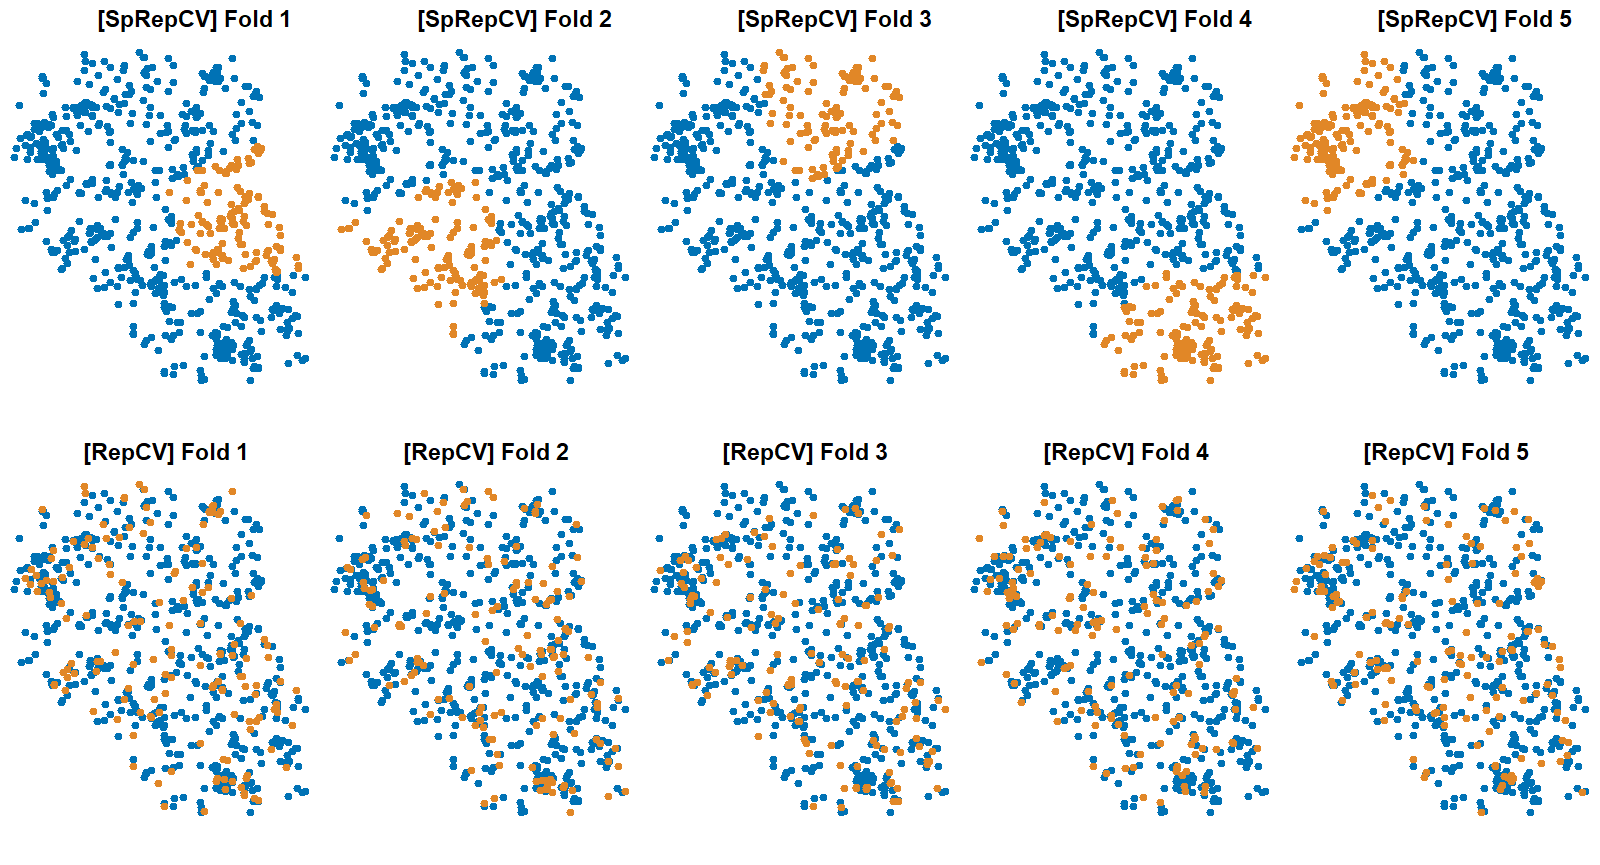
\includegraphics[width=1\textwidth,height=\textheight]{figures/spcv_plot.png}

}

\caption{\label{fig-rycina-spcv}Porównanie przestrzennego i losowego
podziału zbioru danych na potrzeby walidacji krzyżowej jednego
powtórzenia. Podział przestrzenny (górny rząd) i losowy (dolny rząd).
Niebieskie punkty reprezentują dane treningowe, a pomarańczowe dane
testowe. Opracowanie własne na podstawie Schratz,
\href{https://mlr.mlr-org.com/articles/tutorial/handling_of_spatial_data.html}{2021}}

\end{figure}

W niniejszej pracy przestrzenna walidacja krzyżowa została wykorzystana
do dwóch celów: optymalizacji hiperparametrów (sekcja \ref{sec-tuning})
oraz oceny jakości modeli (sekcja \ref{sec-model-quality-assessment}).

\hypertarget{sec-tuning}{%
\subsection{Dostrajanie modeli}\label{sec-tuning}}

Większość algorytmów uczenia maszynowego wymaga ustalenia wartości
pewnych zmiennych konfiguracyjnych zwanych hiperparametrami
\autocite{krol_2022_podstawy_ml}. Hiperparametry są ustawiane przed
rozpoczęciem procesu uczenia, nie uzyskuje się ich w wyniku trenowania
modelu ani nie są modyfikowane w trakcie wykonywania algorytmu
\autocite{krol_2022_podstawy_ml}. Optymalna konfiguracja hiperparametrów
jest zwykle znajdowana w określonej przestrzeni poszukiwań (ang.
\emph{search space}) i może być ustalana np. na podstawie zagnieżdżonej
walidacji krzyżowej (ang. \emph{nested cross-validation})
\autocite{lovelace_2019_geocomputation}. Optymalizacja hiperparametrów
(ang. \emph{hyperparameters}) odgrywa kluczową rolę w osiągnięciu
najwyższej mocy predykcyjnej i jakości modelu
\autocite{schratz_2019_hyperparameters}, a jej celem jest znalezienie
optymalnej konfiguracji hiperparametrów algorytmu uczenia maszynowego
dla danego zadania \autocite{bischl_2024_mlr3}.

Wykorzystanie tych samych danych do oceny jakości i dostrajania mogłoby
potencjalnie prowadzić do nadmiernie wysokich wyników oceny jakości,
czego można uniknąć, stosując zagnieżdżoną przestrzenną kroswalidację.
Metoda przestrzennej zagnieżdżonej walidacji krzyżowej to rozwinięcie
przestrzennej walidacji krzyżowej (sekcja \ref{sec-spcv}), przeznaczone
do procesu strojenia hiperparametrów. Każdy podzbiór (\emph{fold})
utworzony w przestrzennej walidacji krzyżowej jest dzielony na kolejne,
zewnętrzne i wewnętrzne podzbiory. W zewnętrznym obiegu model jest
trenowany na danych z jednego obszaru przestrzennego i testowany na
innym, podczas gdy wewnętrzny obieg służy do doboru optymalnych
hiperparametrów. Cały proces jest następnie powtarzany na każdym z
\emph{k} zewnętrznych podzbiorów, co prowadzi do określenia najlepszego
ustawienia hiperparametrów.

Hiperparametry \texttt{mtry}, \texttt{sample.fraction} i
\texttt{min.node.size} są parametrami określającymi stopień losowości
lasu losowego i powinny zostać odpowiednio dostrojone
\autocite{probst_2019_hyperparameters}. Liczba losowo wybranych
zmiennych, \texttt{mtry}, wskazuje, ile predyktorów powinno zostać
użytych w każdym drzewie, a parametr \texttt{sample.fraction} odnosi się
do wielkości próby, czyli ułamka obserwacji użytego w każdym drzewie
\autocite{lovelace_2019_geocomputation}. Mniejsza wielkość próby
prowadzi do większej różnorodności drzew, a tym samym do mniejszej
korelacji między nimi, co pozytywnie wpływa na dokładność predykcji przy
agregacji drzew \autocite{probst_2019_hyperparameters}. Minimalna
wielkość węzła \texttt{min.node.size} określa minimalną liczbę
obserwacji w węźle końcowym \autocite{probst_2019_hyperparameters}. W
ramach optymalizacji uwzględniono również parametry \texttt{num.trees}
oraz \texttt{max.depth}, odnoszące się odpowiednio do liczby drzew w
lesie oraz maksymalnej głębokości pojedynczego drzewa.

Kombinacje hiperparametrów zostały wybrane losowo w ramach określonych
granic strojenia ustalonych za pomocą pakietu R \emph{paradox}
\autocite{R-paradox}. Zasięg przestrzeni strojenia został wybrany
zgodnie z wartościami zalecanymi w dedykowanym do tego pakiecie R
\emph{mlr3tuningspaces} \autocite{R-mlr3tuningspaces} oraz literaturze
\autocite{probst_2019_hyperparameters,schratz_2019_hyperparameters}.
\texttt{mtry} powinno przyjmować wartości z przedziału od 1 do liczby
predyktorów, \texttt{sample.fraction} powinno mieścić się w zakresie od
0,2 do 0,9, a \texttt{min.node.size} powinno przybierać wartości z
przedziału od 1 do 10. Zgodnie z pakietem R \emph{mlr3tuningspaces}
\autocite{R-mlr3tuningspaces}, hiperparametr \texttt{num.trees} powinien
być ustawiony w zakresie od 1 do 2000, jednak ograniczono jego wartości
do przedziału od 50 do 500 w celu zwiększenia wydajności obliczeń.

\hypertarget{tbl-tabela-tuning}{}
\begin{table}
\caption{\label{tbl-tabela-tuning}Optymalne hiperparametry otrzymane w wyniku dostrajania modeli RF }\tabularnewline

\centering
\begin{tabular}{ccccccc}
\toprule
\multicolumn{1}{c}{ } & \multicolumn{5}{c}{Optymalizowane parametry} & \multicolumn{1}{c}{ } \\
\cmidrule(l{3pt}r{3pt}){2-6}
Wariant \textsuperscript{a} & mtry & sample.fraction & min.node.size & num.trees & max.depth & AUC\\
\midrule
1 & 6 & 0.6689 & 2 & 264 & 34 & 0.9842\\
2 & 7 & 0.7373 & 1 & 372 & 23 & 0.9914\\
3 & 7 & 0.8847 & 5 & 388 & 75 & 0.9904\\
4 & 6 & 0.8758 & 5 & 291 & 54 & 0.9881\\
5 & 5 & 0.6898 & 1 & 234 & 99 & 0.9850\\
6 & 8 & 0.8847 & 5 & 388 & 75 & 0.9905\\
\bottomrule
\multicolumn{7}{l}{\textsuperscript{a} Patrz: tabela 3.1}\\
\end{tabular}
\end{table}

Optymalne hiperparametry uzyskane w wyniku dostrajania modeli lasów
losowych dla poszczególnych wariantów (zbiorów danych) razem z oceną
jakości AUC\footnote{Pole powierzchni pod krzywą (ang. \emph{Area Under
  Curve} lub \emph{Area Under the ROC Curve}, AUC lub AUROC) to miara
  jakości modelu, obliczająca obszar pod krzywą ROC (ang. \emph{receiver
  operating characteristic curve}), która graficznie przedstawia
  zależność pomiędzy czułością (\emph{true positive rate}) a
  specyficznością (\emph{false positive rate})
  \autocite{jaworski_2013_perfomance_measures}. AUC reprezentuje
  zdolność klasyfikatora binarnego do oddzielania klas pozytywnych od
  klas negatywnych. Wartości AUC mieszczą się w zakresie od 0 do 1,
  gdzie wartość 0,5 lub niższa oznacza model nie lepszy od losowego, a
  1,0 -- doskonałe przewidywanie obu klas.} zostały przedstawione w
tabeli \ref{tbl-tabela-tuning}. Warto zauważyć, że warianty 3 i 6
wykazują identyczne wartości dla parametrów \texttt{sample.fraction},
\texttt{min.node.size}, \texttt{num.trees} i \texttt{max.depth}. Podczas
losowania hiperparametrów dla każdego wariantu wykorzystano to samo
ziarno losowości (ang. \emph{random seed}), ustawione za pomocą funkcji
\texttt{set.seed()}. Dla dwóch wspomnianych wariantów najlepsze wyniki
zostały osiągnięte przy wykorzystaniu identycznego zestawu czterech z
pięciu optymalizowanych hiperparametrów.

Warto dodać, że lasy losowe często wykazują satysfakcjonujące wyniki
nawet z domyślnymi wartościami hiperparametrów, co może być jednym z
powodów ich dużej popularności \autocite{lovelace_2019_geocomputation}.
Chociaż dostrojenie lasów losowych powinno poprawiać jakość modeli,
korzyści ze strojenia są znacznie mniejsze w porównaniu do innych
algorytmów uczenia maszynowego, takich jak maszyny wektorów nośnych
(ang. \emph{Support Vector Machines}, SVM \autocite{svm})
\autocite{probst_2019_hyperparameters} czy XGBoost \autocite{xgboost}.

\hypertarget{sec-model-quality-assessment}{%
\subsection{Ocena jakości modeli}\label{sec-model-quality-assessment}}

Macierz błędów (ang. \emph{error matrix} lub \emph{confusion matrix}) to
tablica prezentująca wyniki klasyfikatora binarnego, podając informację
o liczbie obiektów przypisanych do każdej z klas. Macierz błędów jest
wynikiem porównania prognozy (klasyfikacji) z rzeczywistymi danymi,
składając się z czterech wartości reprezentujących różne kombinacje
przewidywanych i rzeczywistych klas.

W macierzy błędów dwie wartości reprezentują predykcje pozytywne:
przypadki prawdziwie pozytywne (ang. \emph{true positive}, TP) opisują
sytuacje, w których klasyfikator poprawnie przewidział daną klasę jako
pozytywną, natomiast przypadki prawdziwie negatywne (ang. \emph{true
negative}, TN) opisują poprawne przewidywanie klasy negatywnej. Dwie
pozostałe wartości informują o błędnie sklasyfikowanych przypadkach:
przypadki fałszywie pozytywne (ang. \emph{false positive}, FP) opisują
sytuacje, w których klasyfikator błędnie wskazał klasę pozytywną,
podczas gdy rzeczywiście była ona negatywna. Przypadki fałszywie
negatywne (ang. \emph{false negative}, FN) to natomiast sytuacje, w
których klasyfikator błędnie przewidział klasę jako negatywną, gdy
faktycznie była ona pozytywna.

Ocenę klasyfikatorów stworzonych w niniejszym badaniu przeprowadzono
przy użyciu macierzy błędów oraz trzech miar jakości dostosowanych do
klasyfikatorów binarnych:

\begin{itemize}
\item
  Precyzja (ang. \emph{precision}, inaczej \emph{positive predictive
  value}) - określa jaka część wyników wskazanych przez klasyfikator
  jako pozytywne jest faktycznie pozytywna
  \autocite{jaworski_2013_perfomance_measures}
\item
  Czułość (ang. \emph{sensitivity}, inaczej \emph{recall} lub \emph{true
  positive rate}) - określa jaką część prawdziwie pozytywnych wyników
  wykrył klasyfikator \autocite{jaworski_2013_perfomance_measures}
\item
  F1-score - średnia harmoniczna pomiędzy precyzją i czułością,
  umożliwiająca ocenę równowagi między tymi miarami, która w pewnym
  stopniu opisuje całościowo wynik. Miara ta nie uwzględnia wyników
  prawdziwie negatywnych \autocite{zygierewicz_2021_ml}.
\end{itemize}

Wartości każdej z wymienionych miar jakości modelu zawierają się w
zakresie od 0 do 1, gdzie wartość 0 reprezentuje niską jakość modelu,
natomiast wartość 1 odzwierciedla wysoki poziom jakości.

Macierz błędów oraz wymienione miary jakości zostały zastosowane zarówno
w ocenie jakości modeli na podstawie próby (danych treningowych), jak i
w ocenie ostatecznych wyników klasyfikacji dla całego obszaru badań
(populacji).

\hypertarget{sec-variable-importance}{%
\section{Ważność zmiennych}\label{sec-variable-importance}}

Ocena ważności zmiennych (ang. \emph{variable importance}) jest
elementem oceny jakości stworzonych modeli. Analiza wpływu
poszczególnych zmiennych na dokładność modelu pozwala ocenić, które
zmienne są istotne dla przewidywań. Stosowanie zmiennych o niskiej mocy
predykcyjnej może prowadzić do nadmiernego dopasowania (ang.
\emph{overfitting}) modelu lub obniżenia jego jakości. Dlatego istotny
jest wybór odpowiednich zmiennych do trenowania modelu, unikając na
przykład kolinearności predyktorów, czyli wysokiej korelacji między
zmiennymi.

W lasach losowych ważność zmiennych można ocenić różnymi metodami, z
których dwie najpopularniejsze to miara zanieczyszczenia Giniego (ang.
\emph{Gini impurity}) oraz metoda oparta na permutacji
\autocite{biecek_2017_przewodnik}. W celu określenia wartości zmiennych
wykorzystywanych do identyfikacji farm fotowoltaicznych na podstawie
danych teledetekcyjnych zastosowano metodę permutacji, która może być
również używana do upraszczania i eksploracji modeli lub generowania
wiedzy \autocite{biecek_2021_model_analysis}.

Główną ideą metody opartej na permutacji jest pomiar tego, jak bardzo
zmieni się dopasowanie modelu, gdy usunięty zostanie wpływ wybranej
zmiennej lub grupy zmiennych. Jeśli zmienna jest istotna, permutacja jej
wartości skutkuje pogorszeniem jakości modelu. Im większa zmiana
dopasowania modelu, tym istotniejsza jest permutowana zmienna
\autocite{biecek_2021_model_analysis}. Metoda oparta na permutacji
została pierwotnie zaproponowana przez Breimana
\autocite*{breiman_2001_rf} dla lasów losowych, jednak jej prostota
umożliwia zastosowanie permutacji do dowolnego modelu, a także
porównywanie ważności zmiennych pomiędzy modelami o różnych strukturach
\autocite{biecek_2021_model_analysis}.

W przypadku silnie skorelowanych ze sobą zmiennych, brak jednej z nich
niekoniecznie będzie negatywnie wpływać na jakość modelu, ponieważ inna,
silnie skorelowana zmienna może zastąpić tę brakującą informację
\autocite{biecek_2021_model_analysis}. Macierz korelacji zmiennych
użytych w tym badaniu (rycina \ref{fig-variables-correlation}) ukazuje
silne związki między niektórymi zmiennymi. Wysoka korelacja występuje
szczególnie między pasmami Sentinel-2 w zakresie widzialnym (kanały
B02-04) a pasmami średniej podczerwieni (kanały B11-12). Zauważalna jest
również wysoka korelacja między pasmami czerwieni krawędziowej (kanały
B05-07) oraz bliskiej podczerwieni (kanały B08 i B8A). Wykorzystane
polaryzacje Sentinel-1 również są ze sobą skorelowane. Wskaźniki
teledetekcyjne wykazują zazwyczaj znaczną dodatnią lub ujemną korelację
z pasmami, które zostały wykorzystane do ich obliczenia. Tekstury obrazu
charakteryzują się natomiast wysoką dodatnią korelacją ze zmiennymi, dla
których zostały one określone.

\begin{figure}[t]

{\centering 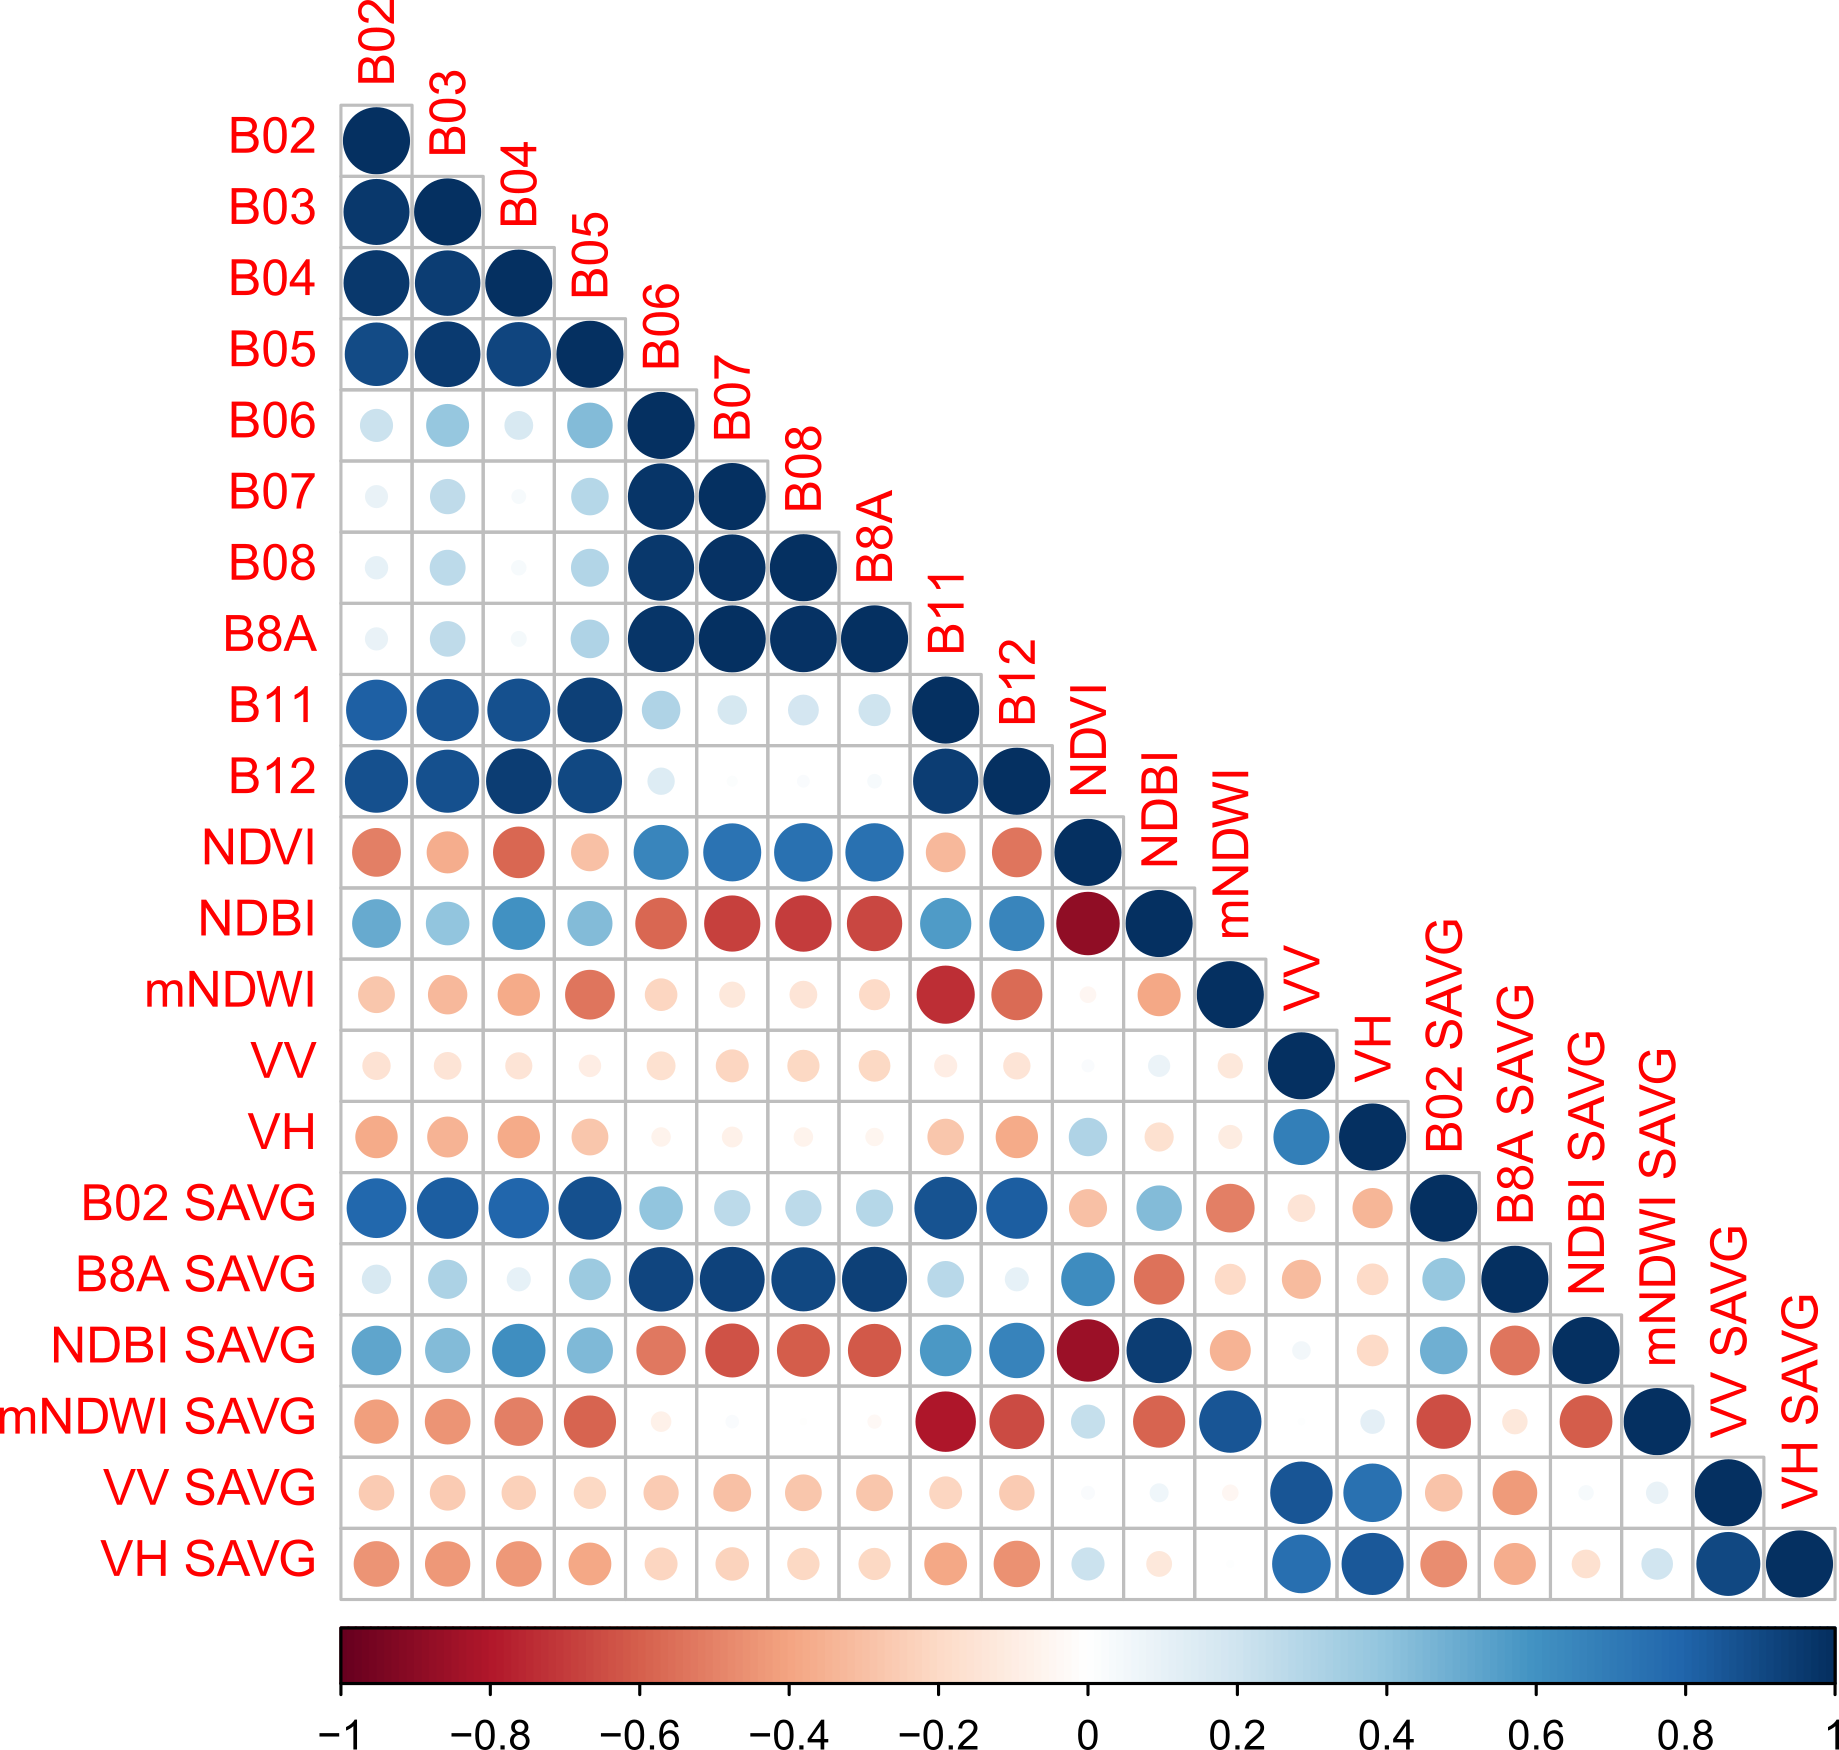
\includegraphics[width=0.9\textwidth,height=\textheight]{figures/corrplot1.png}

}

\caption{\label{fig-variables-correlation}Macierz korelacji wszystkich
zmiennych wykorzystanych w badaniu}

\end{figure}

\hypertarget{sec-post-processing}{%
\section{Przetwarzanie końcowe}\label{sec-post-processing}}

Ostatnim etapem procesu detekcji farm fotowoltaicznych było określenie
metod przetwarzania końcowego (ang. \emph{post-processing}), mających na
celu udoskonalenie wyników wykrywania farm fotowoltaicznych. Z
teoretycznego punktu widzenia, obszar zajmowany przez farmę
fotowoltaiczną lub jej fragmenty powinien być większy niż powierzchnia
pojedynczej komórki lub grupy kilku komórek. W celu usunięcia
pozytywnych predykcji, które reprezentowały pojedyncze komórki lub
obszary składające się z 10 lub mniej komórek (czyli o powierzchni
mniejszej/równej 1000 m\textsuperscript{2}) zastosowano sekwencję
procesów przetwarzania, dzięki której udało się pozbyć tzw. efektu soli
i pieprzu (ang. \emph{salt-and-pepper effect}).

\begin{figure}[t]

{\centering 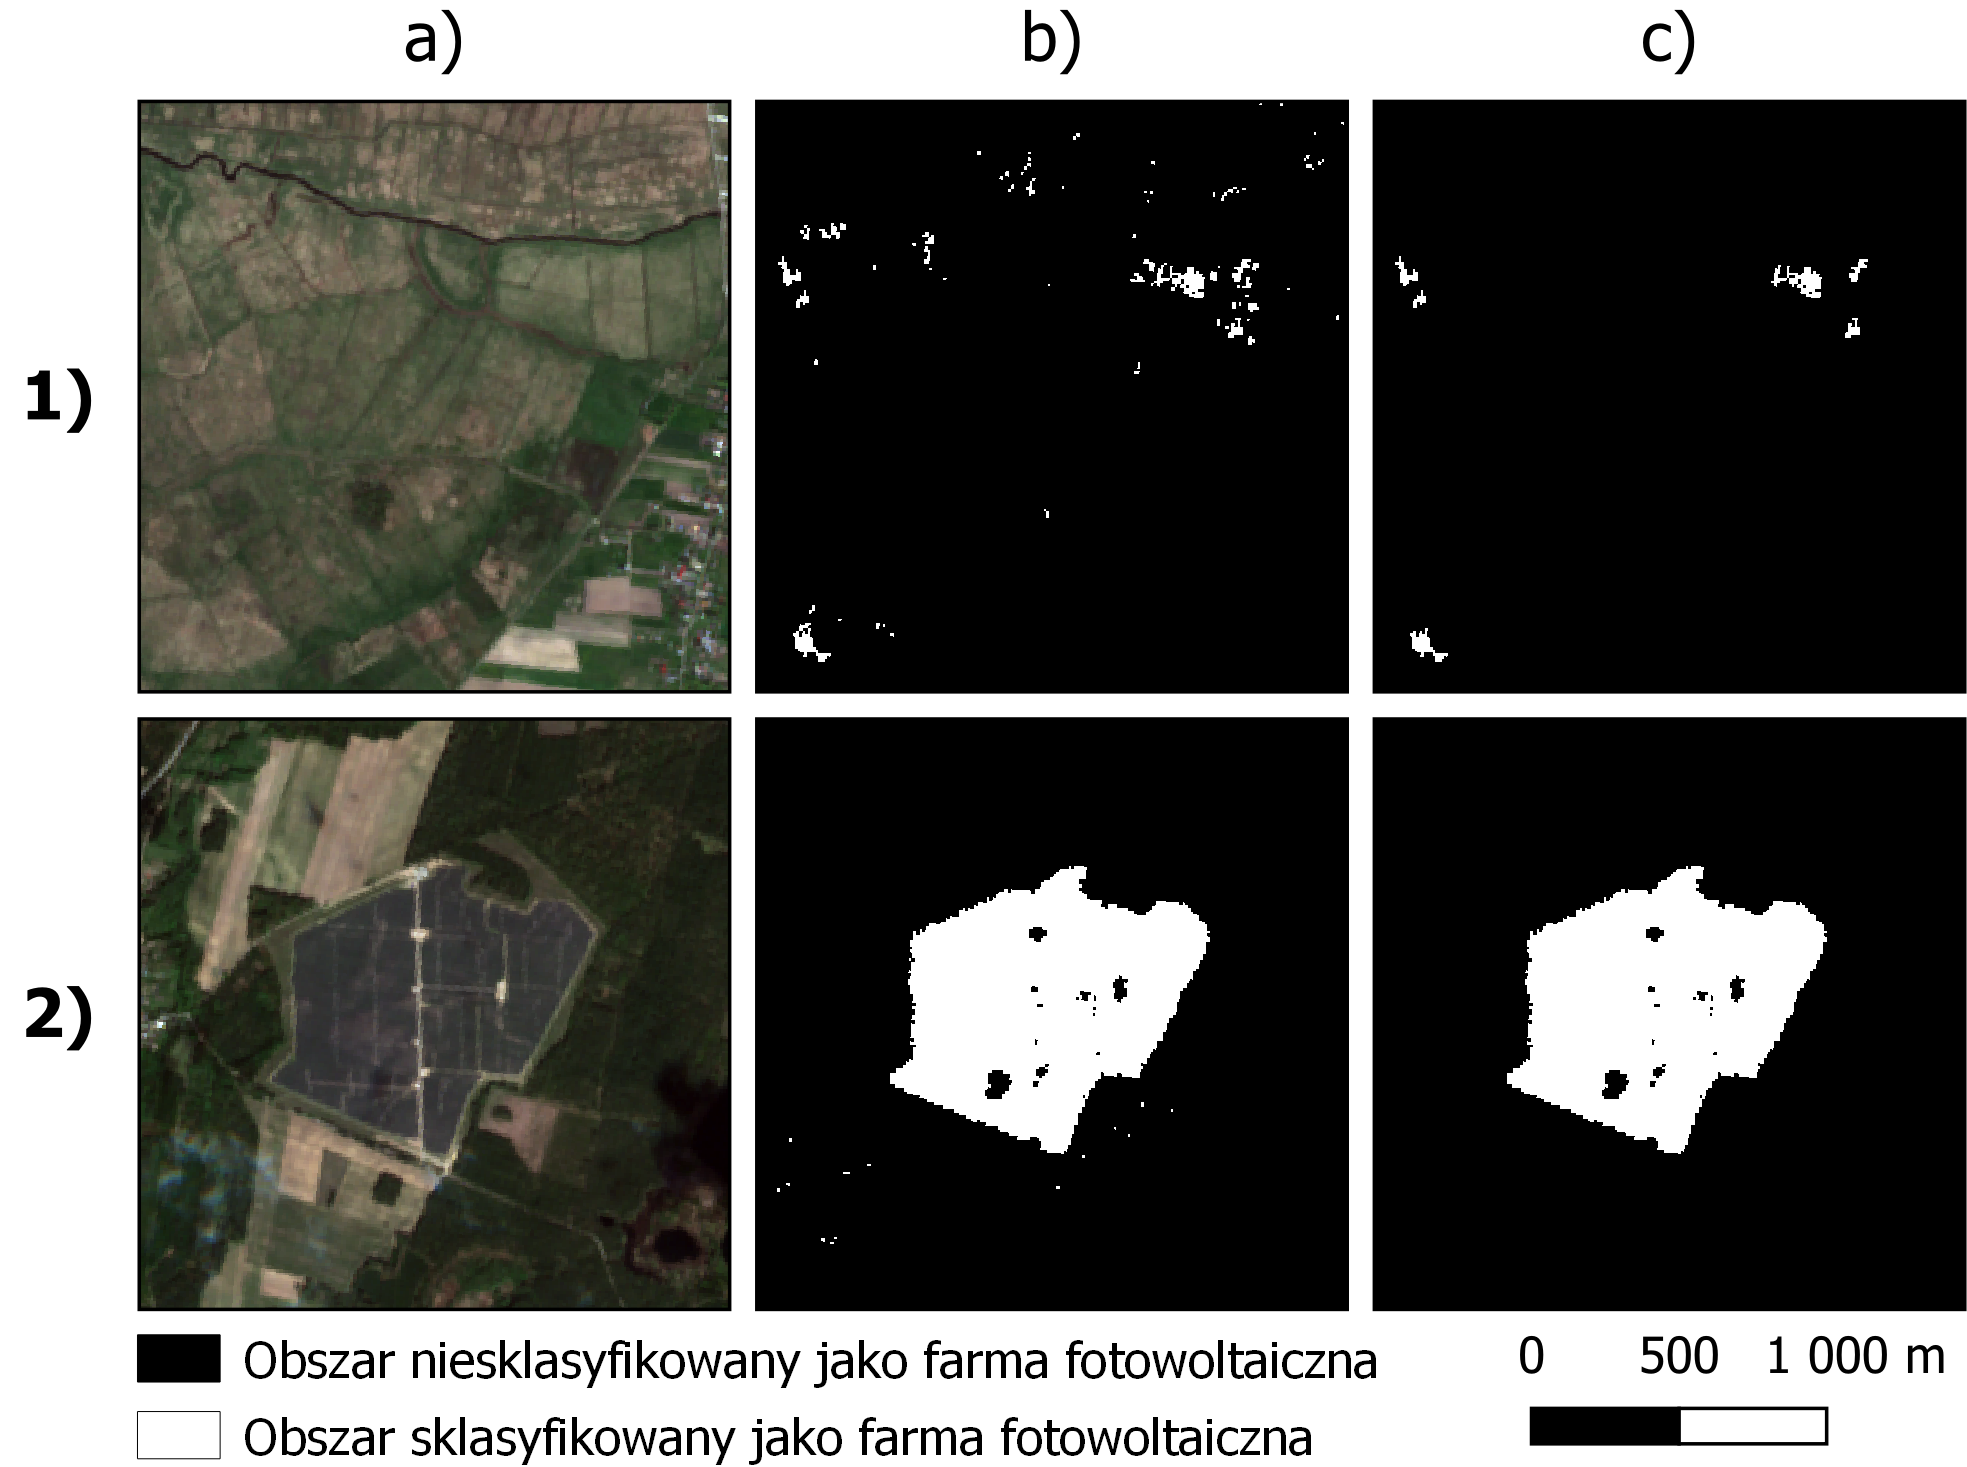
\includegraphics[width=1\textwidth,height=\textheight]{figures/postprocessing_pl.png}

}

\caption{\label{fig-rycina-post-processing}Kompozycja RGB Sentinel-2
(a), wstępne wyniki detekcji PV przed przetwarzaniem końcowym (b), PV
wykryte po przetwarzaniu końcowym (c) w przypadku niepoprawnej (1) i
poprawnej (2) predykcji dla wariantu nr 1}

\end{figure}

Przetwarzanie końcowe obejmowało wektoryzację rastrowych wyników
predykcji dla każdego wariantu, a następnie selekcję pozytywnych
predykcji oraz obliczenie powierzchni każdego wybranego obszaru. Na
podstawie obliczonej powierzchni usunięto wszystkie pozytywne predykcje
reprezentujące pojedyncze komórki lub obszary składające się z 10 lub
mniej komórek, dzięki czemu wiele błędnych predykcji zostało usuniętych.
W rezultacie uzyskano końcowy produkt wykrywania farm fotowoltaicznych
oparty na danych teledetekcyjnych w formie wektorowej.

W celu stworzenia wizualizacji oraz porównania produktów końcowych z
predykcjami niepoddanymi etapowi przetwarzania końcowego produkty
wektorowe zostały ponownie przetworzone do formy rastrowej. Efekty
zastosowanego przetwarzania końcowego przedstawia rycina
\ref{fig-rycina-post-processing}.

\hypertarget{oprogramowanie}{%
\section{Oprogramowanie}\label{oprogramowanie}}

\hypertarget{qgis}{%
\subsection{QGIS}\label{qgis}}

QGIS \autocite{qgis}, to wieloplatformowe i wolne oprogramowanie o
otwartym kodzie źródłowym przeznaczone do przetwarzania danych
przestrzennych, rozwijane od 2002 roku
\autocite{hejmanowska_2020_dane,flenniken_2020_qgis}. Algorytmy
przetwarzania danych przestrzennych zebrane w oprogramowaniu QGIS
umożliwiają manipulację danymi rastrowymi oraz wektorowymi, a także
prowadzenie analiz i wizualizację wyników
\autocite{hejmanowska_2020_dane}. Oprogramowanie QGIS oferuje również
możliwość korzystania z wielu zewnętrznych programów, tzw. wtyczek (ang.
\emph{plug-in}) rozszerzających jego funkcjonalność
\autocite{hejmanowska_2020_dane}. W repozytorium wtyczek znaleźć można
narzędzia do zarządzania danymi, przetwarzania obrazów, wizualizacji,
czy wykonania dodatkowych zadań, takich jak np. nadawanie georeferencji
czy klasyfikacja zobrazowań satelitarnych
\autocite{hejmanowska_2020_dane}. QGIS dostarcza także zaawansowane
narzędzia do digitalizacji, umożliwiające rysowanie i edytowanie
obiektów wektorowych oraz pozwala na przeglądanie danych przestrzennych
dostępnych w Internecie za pomocą usług sieciowych, takich jak WMS, WMTS
czy XYZ Tiles.

Oprogramowanie QGIS zostało wykorzystane w tej pracy do stworzenia
zestawu danych referencyjnych poprzez wizualną interpretację
ortofotomapy oraz mozaik satelitarnych, na podstawie których dokonano
digitalizacji farm fotowoltaicznych istniejących na obszarze badań. QGIS
posłużył również do stworzenia końcowych wizualizacji (map)
prezentowanych w niniejszej pracy.

\hypertarget{sentinel-1-toolbox-i-snap}{%
\subsection{Sentinel-1 Toolbox i SNAP}\label{sentinel-1-toolbox-i-snap}}

Przetwarzanie danych pochodzących z misji Sentinel-1 umożliwia zestaw
narzędzi Sentinel-1 Toolbox (S1TBX) \autocite{s1tbx}, przeznaczony do
obsługi danych radarowych. Zestaw narzędzi S1TBX zawiera narzędzia do
kalibracji, filtrowania plamek (tzw. efektu pieprzu i soli),
koregistracji, ortorektyfikacji, mozaikowania, konwersji danych,
polarymetrii czy interferometrii \autocite{sentinel-1-toolbox}.
Sentinel-1 Toolbox jest opracowywany dla ESA przez firmę Array we
współpracy z DLR, Brockmann Consult i OceanDataLab
\autocite{sentinel-1-toolbox}.

SNAP \autocite{snap}, czyli Sentinel Application Platform to platforma
oprogramowania rozwijana wspólnie przez firmy Brockmann Consult,
SkyWatch i C-S na zlecenie Europejskiej Agencji Kosmicznej, przeznaczona
do naukowego wykorzystania misji optycznych i mikrofalowych Sentinel
\autocite{snap-desktop,esa_snap}. Oprogramowanie SNAP zawiera zestawy
narzędzi do wizualizacji, przetwarzania oraz analizy danych
teledetekcyjnych, a także umożliwia tworzenie łańcuchów procesów
przetwarzania danych zdefiniowanych przez użytkownika
\autocite{hejmanowska_2020_dane,moskolai_2022_s1_workflow}.

\hypertarget{ux15brodowisko-jux119zyka-r}{%
\subsection{Środowisko języka R}\label{ux15brodowisko-jux119zyka-r}}

Czynności związane z końcowym przygotowaniem danych wejściowych oraz
bezpośrednio z uczeniem maszynowym zostały wykonane z wykorzystaniem
środowiska języka R \autocite{R-base}. R to wieloplatformowy język
programowania o otwartym kodzie źródłowym do obliczeń statystycznych i
wizualizacji danych. Dzięki dużej liczbie pakietów R obsługuje również
statystki geoprzestrzenne, modelowanie oraz wizualizację danych
przestrzennych \autocite{lovelace_2019_geocomputation}. W pracy
wykorzystane zostało zintegrowane środowisko programistyczne (ang.
\emph{Integrated Development Environment}, IDE) RStudio
\autocite{rstudio_team_2020_rstudio} przeznaczone dla języka R. Poza
standardowymi możliwościami środowiska R, w procesie pracy wykorzystane
zostały pakiety stworzone przez społeczność R w celu rozszerzenia
funkcjonalności tego języka. Do operacji na danych rastrowych
zastosowano pakiety \emph{terra} \autocite{R-terra} i \emph{stars}
\autocite{R-stars}, natomiast do przetwarzania danych wektorowych
używany był pakiet \emph{sf} \autocite{R-sf}. Obliczanie tekstury obrazu
Sum Average wyprowadzonej z macierzy współwystępowania poziomu szarości
(ang. \emph{gray-level co-occurrence matrix}, GLCM) zostało wykonane
przy pomocy pakietu \emph{GLCMTextures} \autocite{R-GLCMTextures}.
Losowe generowanie danych przestrzennych umożliwił pakiet
\emph{spatstat.random} \autocite{R-spatstat.random} z rodziny pakietów
\emph{spatstat} \autocite{R-spatstat}. Do przeprowadzenia analizy oraz
predykcji opartej o elementy uczenia maszynowego wykorzystano pakiet
\emph{mlr3} \autocite{R-mlr3}, w ramach którego użyty został algorytm
lasów losowych zaimplementowany w pakiecie \emph{ranger}
\autocite{R-ranger}. Podczas strojenia parametrów algorytmów uczenia
maszynowego, korzystano również z pakietu \emph{paradox}
\autocite{R-paradox}, umożliwiającego definiowanie granic przestrzeni
szukania optymalnych wartości hiperparametrów. Do obliczeń związanych z
teksturami obrazu oraz uczeniem maszynowym wykorzystano pakiet
\emph{future} \autocite{R-future}, umożliwiający równoległe
(wielowątkowe) przetwarzanie wyrażeń R, skracające czas realizacji zadań
w stosunku do przetwarzania sekwencyjnego. Wizualizacje przedstawione w
niniejszej pracy zostały utworzone za pomocą pakietów \emph{ggplot2}
\autocite{R-ggplot2}, \emph{spectralR} \autocite{R-spectralR},
\emph{corrplot} \autocite{R-corrplot} oraz \emph{cowplot}
\autocite{R-cowplot}.

\bookmarksetup{startatroot}

\hypertarget{sec-wyniki}{%
\chapter{Wyniki}\label{sec-wyniki}}

\hypertarget{sec-results-model-quality-assessment}{%
\section{Ocena jakości
modeli}\label{sec-results-model-quality-assessment}}

Dla każdego z sześciu wariantów (zestawów danych) przeprowadzono osobną
zagnieżdżoną \emph{k}-krotną przestrzenną walidację krzyżową, zgodnie z
procedurą przestawioną w sekcji \ref{sec-model-quality-assessment}.
Warianty odnoszą się do różnych zestawów zmiennych stworzonych w celu
ustalenia optymalnego zestawu danych na potrzeby detekcji farm
fotowoltaicznych przy wykorzystaniu danych teledetekcyjnych (tabela
\ref{tbl-tabela-datasets}). Zagnieżdżona przestrzenna walidacja krzyżowa
dla każdego z wariantów składała się z kilku etapów, obejmujących
optymalizację hiperparametrów oraz ocenę jakości.

Proces strojenia został skonfigurowany tak, aby generować 1 000 modeli
dla jednego podzbioru w celu określenia optymalnych hiperparametrów.
Powtarzając tę procedurę dla każdego z pięciu ustalonych podzbiorów,
uzyskano łącznie 5 000 modeli w ramach jednego powtórzenia. W celu
identyfikacji optymalnych hiperparametrów założono dwadzieścia iteracji
wymienionych powyżej działań, co doprowadziło do stworzenia łącznie 100
000 modeli.

Zoptymalizowane parametry modelu zostały następnie wykorzystane do
oszacowania jakości modelu, co wymagało dopasowania dodatkowych 100
modeli (5 podzbiorów * 20 powtórzeń). W rezultacie całkowita liczba
stworzonych modeli wykorzystanych do oceny jakości i dostrajania
hiperparametrów dla jednego wariantu wyniosła 100 100.

\hypertarget{tbl-tabela-performance-measures}{}
\begin{table}
\caption{\label{tbl-tabela-performance-measures}Średnie wyniki oceny jakości modeli uzyskane podczas przestrzennej
walidacji krzyżowej }\tabularnewline

\centering
\begin{tabular}{lcccccc}
\toprule
  & Wariant 1 & Wariant 2 & Wariant 3 & Wariant 4 & Wariant 5 & Wariant 6\\
\midrule
Precyzja & 0.8852 & 0.9001 & 0.8746 & 0.9112 & 0.9034 & 0.9180\\
Czułość & 0.7413 & 0.7296 & 0.7181 & 0.7134 & 0.7081 & 0.7151\\
F1-score & 0.7872 & 0.7875 & 0.7691 & 0.7855 & 0.7837 & 0.7929\\
\bottomrule
\end{tabular}
\end{table}

Ocenę klasyfikatorów stworzonych dla każdego z sześciu wariantów (tabela
\ref{tbl-tabela-datasets}) przeprowadzono przy użyciu trzech miar
jakości opisanych w sekcji \ref{sec-model-quality-assessment}. Średnie
wyniki tych miar, oszacowane na podstawie przestrzennej walidacji
krzyżowej, przedstawia tabela \ref{tbl-tabela-performance-measures}.

Ogólnie średnie wartości miar jakości dla każdego z wariantów są
zbliżone. Prawdopodobnie wynika to z faktu, że w każdym wariancie
dziesięć predyktorów uwzględniało dane dotyczące reflektancji Sentinel-2
w jego poszczególnych kanałach. Każdy wariant różnił się jednak od
pozostałych zestawem dodatkowych zmiennych.

Na podstawie średnich wartości miar jakości przedstawionych w tabeli
\ref{tbl-tabela-performance-measures}, najlepsze dopasowanie uzyskano,
wykorzystując wszystkie predyktory (wariant nr 6). Ten wariant osiągnął
najwyższe średnie oceny w dwóch z trzech zastosowanych miar (precyzja i
F1-score). Najlepszy wynik czułości uzyskał natomiast wariant nr 1. W
przypadku dwóch z trzech miar najniższe wyniki odnotowano dla wariantu
nr 3 (precyzja i F1-score), a najgorszą czułością cechuje się natomiast
wariant nr 5.

Rozrzut pomiędzy najlepszym a najgorszym wynikiem dla precyzji wynosi
0,0434, dla czułości 0,0332, a dla F1-score 0,0238. Średnie wyniki
precyzji czterech z sześciu klasyfikatorów przekroczyły wartość 0,90
(0,8746 dla najgorszego wariantu nr 3, 0,9180 dla najlepszego wariantu
nr 6). Wszystkie klasyfikatory uzyskały wyniki czułości na poziomie
wyższym niż 0,70, kształtując się w zakresie od 0,7081 do 0,7413.
Niemniej jednak, takie wyniki czułości wskazują na dość przeciętne
radzenie sobie z wykrywaniem wyników prawdziwie pozytywnych (ang.
\emph{true positive}). Średnie wyniki miary F1-score opisującej
całościowo jakość modelu poprzez ocenę balansu pomiędzy precyzją a
czułością przekroczyły wartość 0,75 dla każdego wariantu, mieszcząc się
w zakresie pomiędzy 0,7691, a 0,7929.

\begin{figure}[t]

{\centering 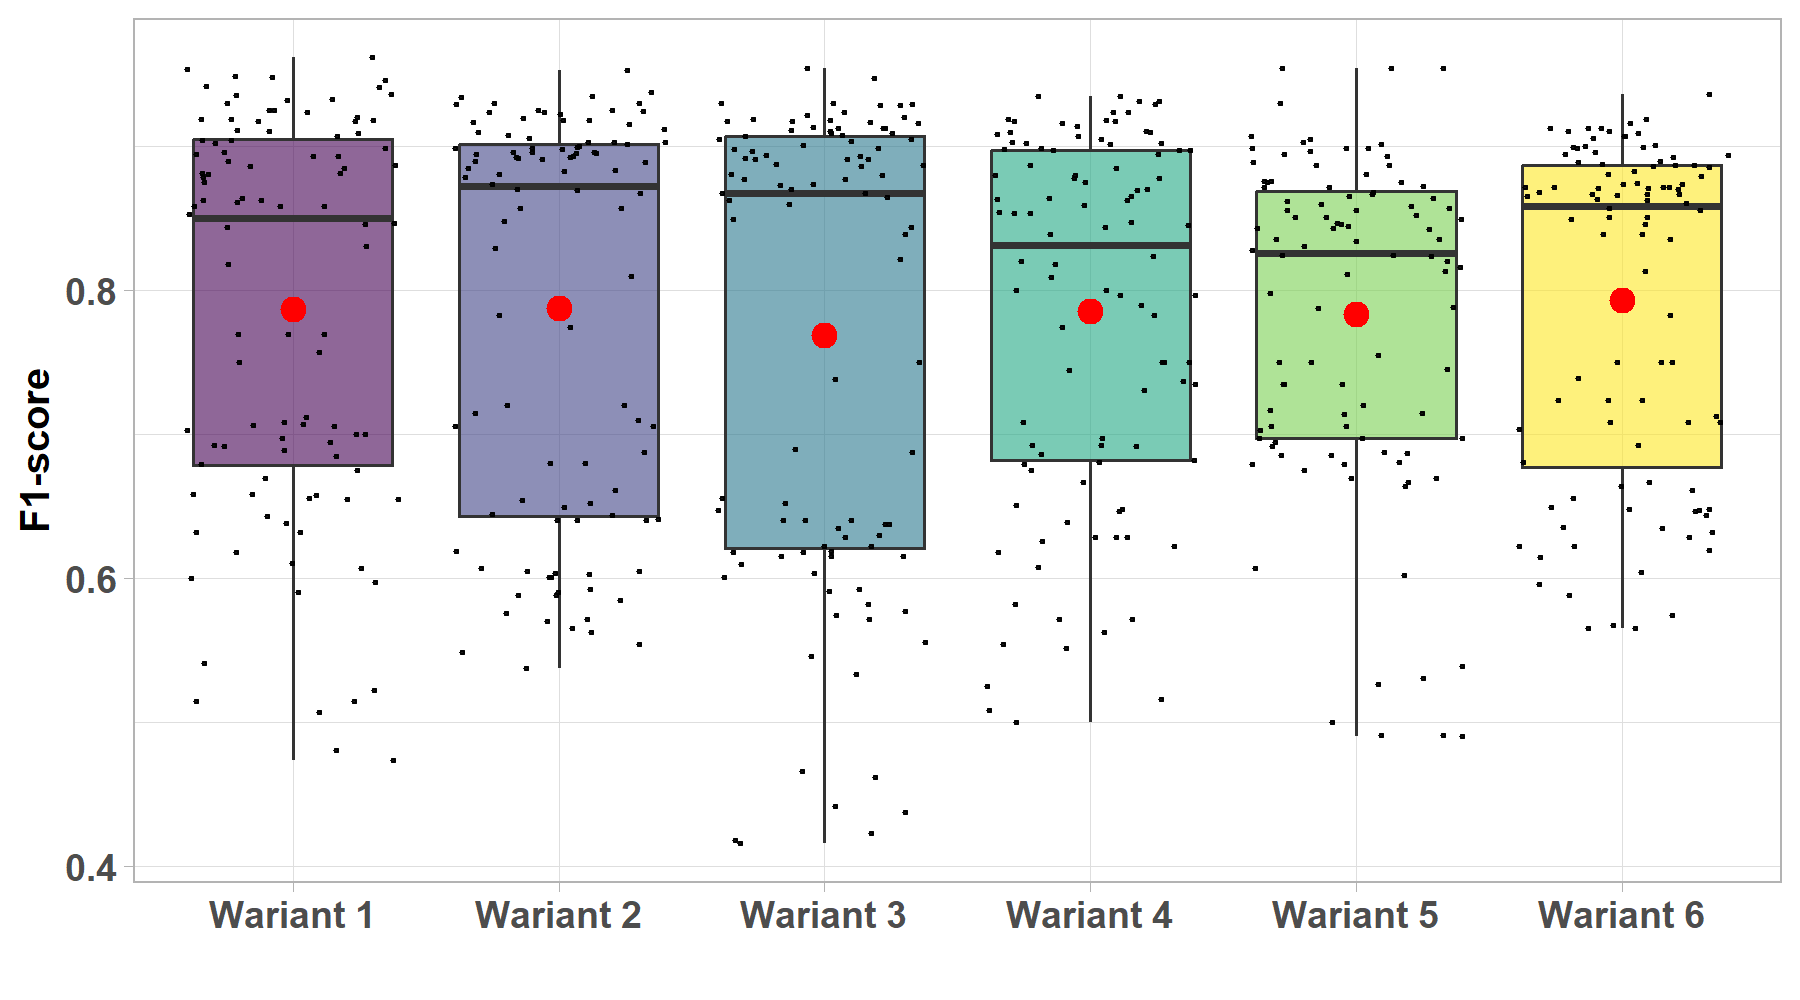
\includegraphics[width=1\textwidth,height=\textheight]{figures/f1_score_boxplot.png}

}

\caption{\label{fig-rycina-f1-score-boxplot}Rozkład wyników miary
F1-score na podstawie 100 modeli dla każdego wariantu. Czerwony punkt
reprezentuje średnią wyników F1-score dla danego wariantu, a~czarne
punkty wyniki dla poszczególnych modeli}

\end{figure}

Stabilność klasyfikatora można ocenić na podstawie rozrzutu wyników
oceny jakości poszczególnych modeli. Im mniej różnorodne są wyniki oceny
jakości modeli w klasyfikatorze, tym bardziej jest on stabilny. Wykres
pudełkowy (rycina \ref{fig-rycina-f1-score-boxplot}) wskazuje, że
wariant o najniższym średnim wyniku F1-score charakteryzuje się również
największym rozrzutem wyników dla poszczególnych modeli. Największą
stabilnością przewidywań charakteryzuje się natomiast wariant nr 6.

Wykres pudełkowy przedstawiający rozkład wyników miary F1-score na
podstawie 100 modeli dla każdego wariantu (rycina
\ref{fig-rycina-f1-score-boxplot}) ujawnia jej bimodalny rozkład wyników
w każdym z wariantów. Charakteryzuje się on grupowaniem wyników wokół
dwóch wartości oddzielonych od siebie, przy czym grupy te nie są równe
pod względem liczebności, ale są wyraźnie większe od pozostałych. Miara
F1-score, będąc średnią harmoniczną precyzji i czułości modelu, jest
silnie zależna od tych dwóch niezależnych miar.

Analiza wyników precyzji ujawniła, że wartości odstające w wynikach tej
miary pochodzą z modeli, gdzie podzbiór testowy składał się głównie z
obserwacji negatywnych, przy niewielkiej liczbie obserwacji pozytywnych.
W przypadku gdy odsetek obserwacji pozytywnych był wyższy, wyniki
precyzji dla danego modelu były bliskie lub równe maksymalnej wartości
jaką może osiągnąć ta miara.

W przeciwieństwie do precyzji, czułość wydaje się być mniej podatna na
wpływ proporcji obserwacji pozytywnych do negatywnych w zbiorze
treningowym. Wyniki czułości dla poszczególnych modeli w każdym z
wariantów, podobnie jak w przypadku F1-score, mają rozkład bimodalny. Z
uwagi na nierównomierne rozmieszczenie próbek reprezentujących farmy
fotowoltaiczne na obszarze badania (rycina
\ref{fig-rycina-spatial-distribution-pv}), zastosowana metoda walidacji
przestrzennej prawdopodobnie nie najlepiej oddaje właściwości
stworzonych modeli, co może stanowić przyczynę bimodalnego rozkładu
wyników czułości i F1-score dla każdego z wariantów.

\hypertarget{sec-results-variable-importance}{%
\section{Ważność zmiennych}\label{sec-results-variable-importance}}

\begin{figure}[t]

{\centering 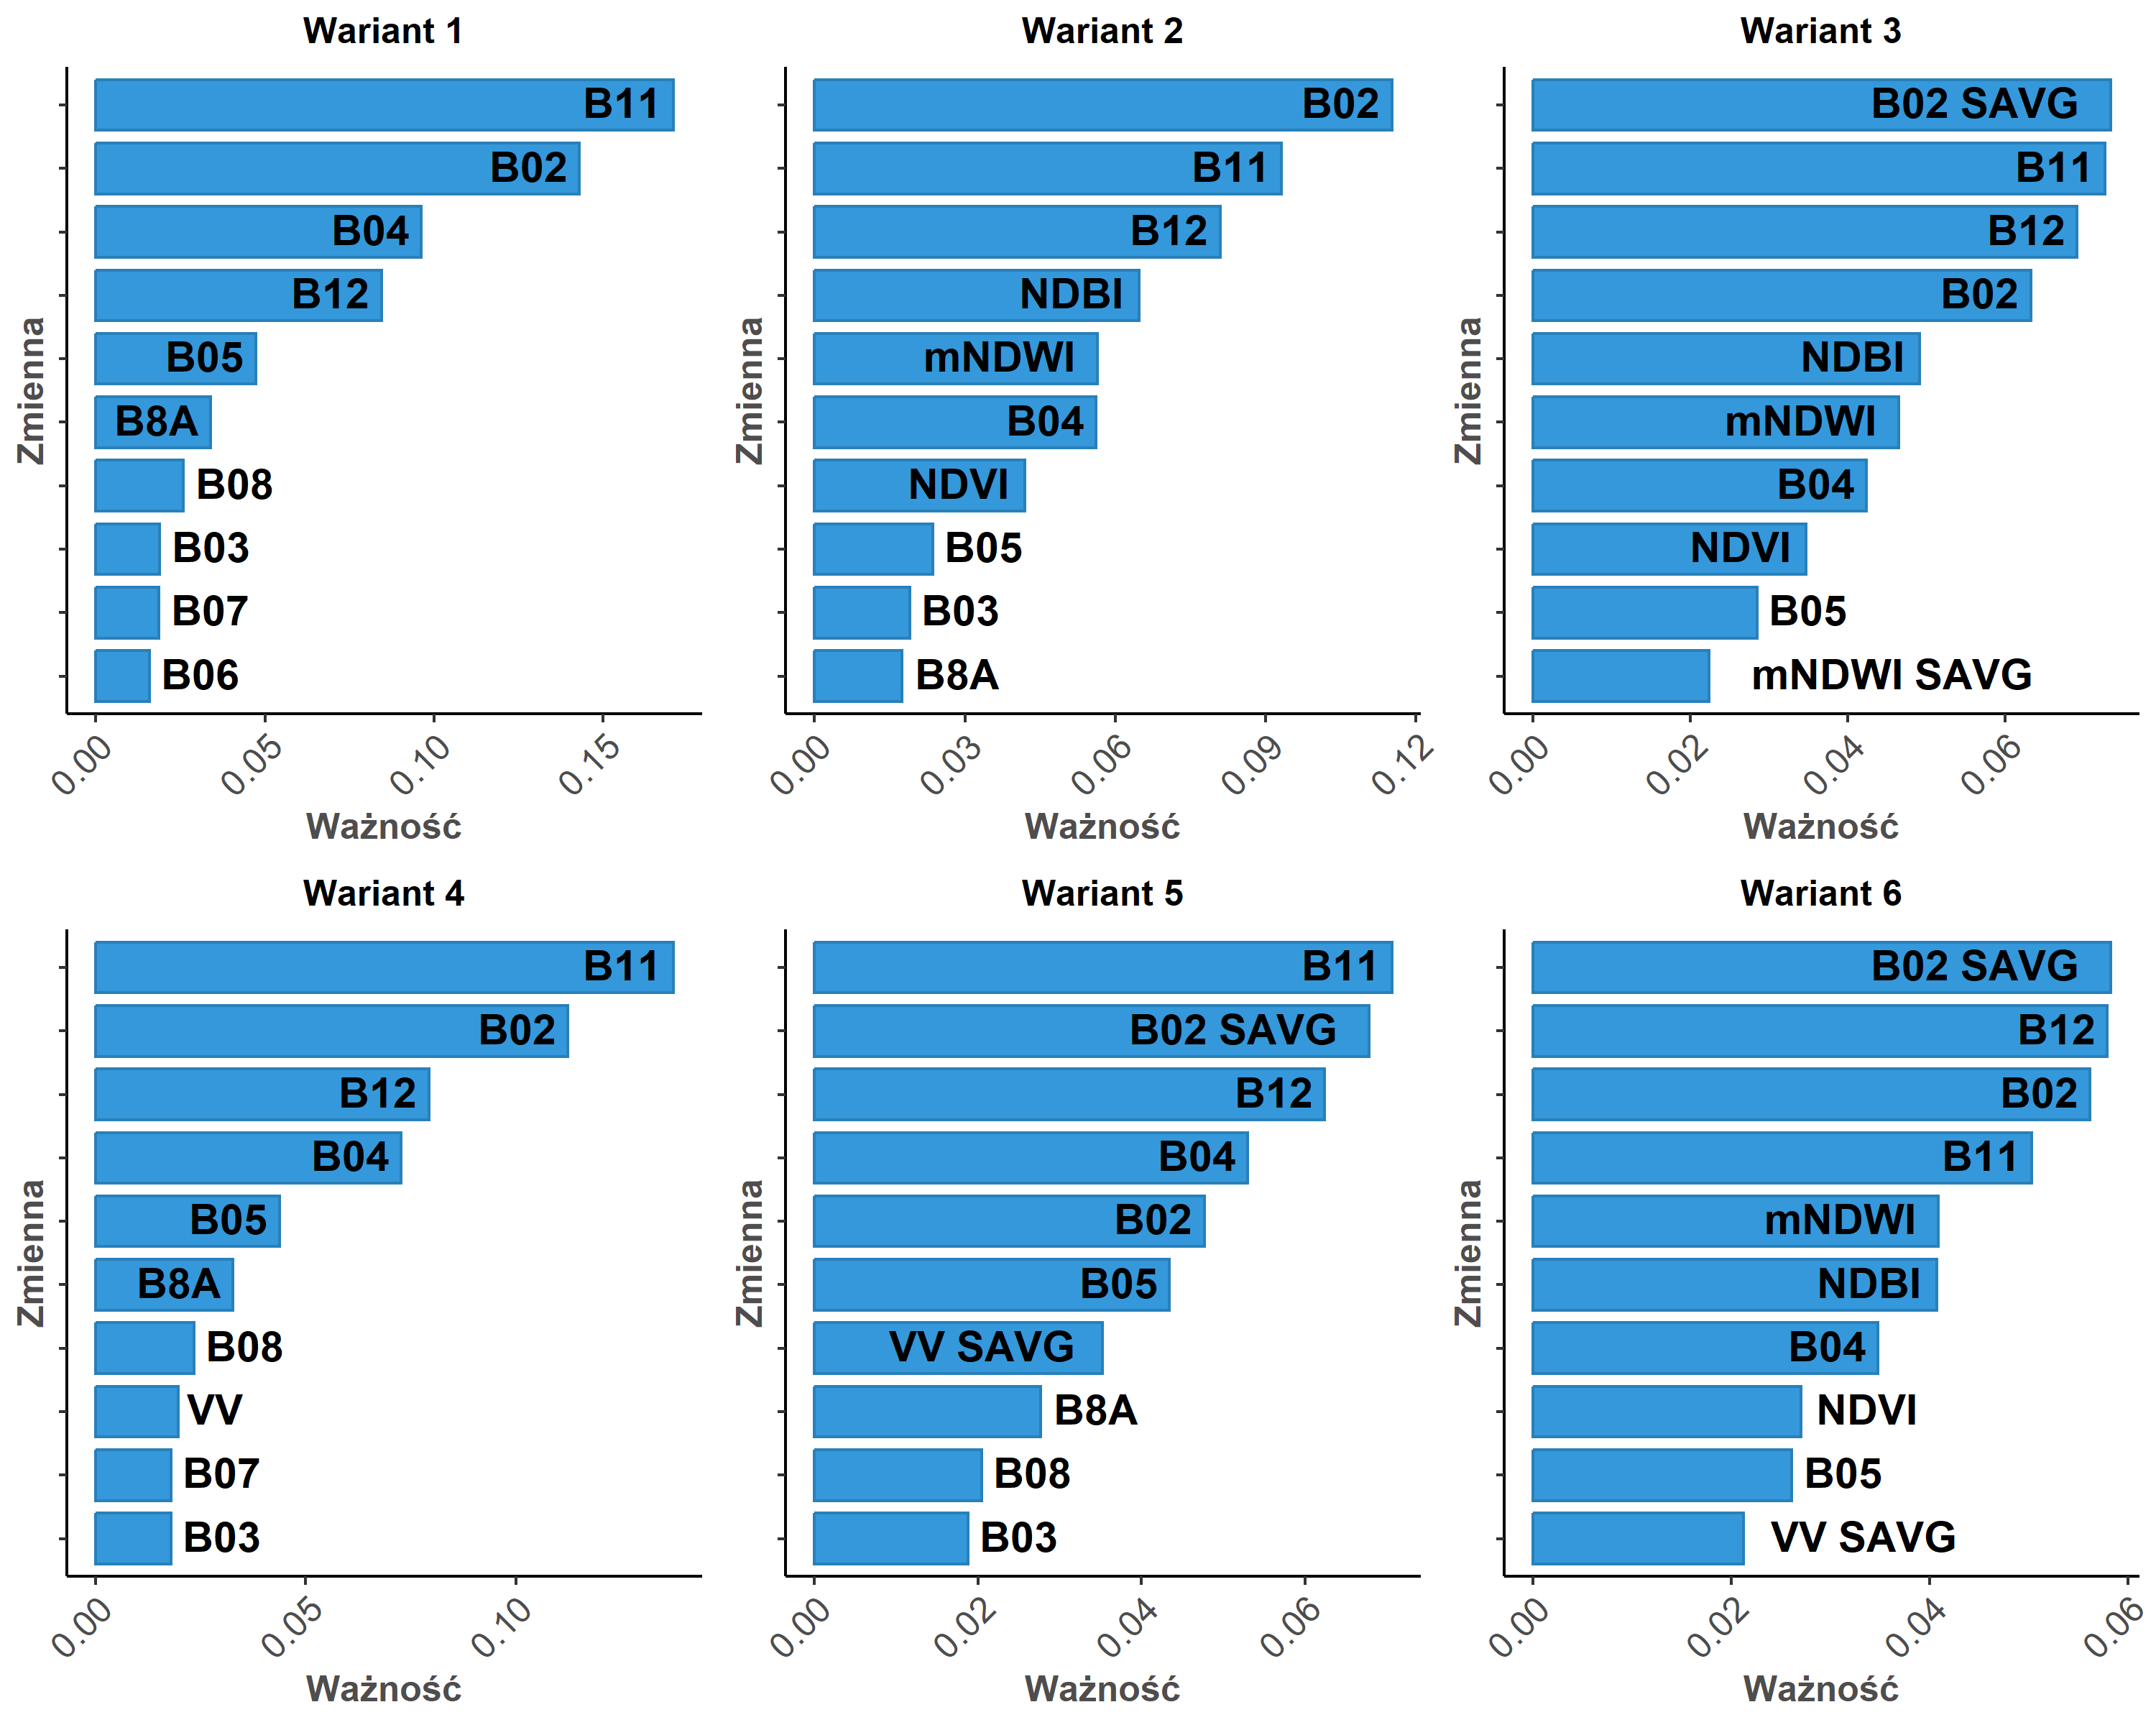
\includegraphics[width=1.05\textwidth,height=\textheight]{figures/importance_cowplot_pl.png}

}

\caption{\label{fig-rycina-variance-importance_cowplot}Permutowana
ważność 10 najważniejszych zmiennych dla każdego wariantu}

\end{figure}

Dla każdego z sześciu wariantów (tabela \ref{tbl-tabela-datasets})
przeprowadzono ocenę ważności zmiennych z wykorzystaniem metody opartej
na permutacji, szczegółowo opisanej w sekcji
\ref{sec-variable-importance}. Ważność zmiennych dla każdego wariantu
została posortowana w porządku malejącym i przedstawiona na rycinie
\ref{fig-rycina-variance-importance_cowplot}, która prezentuje moc
predykcyjną różnych zmiennych wejściowych. Na potrzeby wizualizacji
przedstawiono 10 najważniejszych zmiennych dla każdego wariantu, co
odpowiada liczbie predyktorów w wariancie o najmniejszej ilości
zmiennych (wariant nr 1). Rycina
\ref{fig-rycina-variance-importance-dataset6} ilustruje permutowaną
ważność zmiennych dla wariantu nr 6, obejmującego wszystkie dostępne
zmienne (21 predyktorów).

\begin{figure}[t]

{\centering 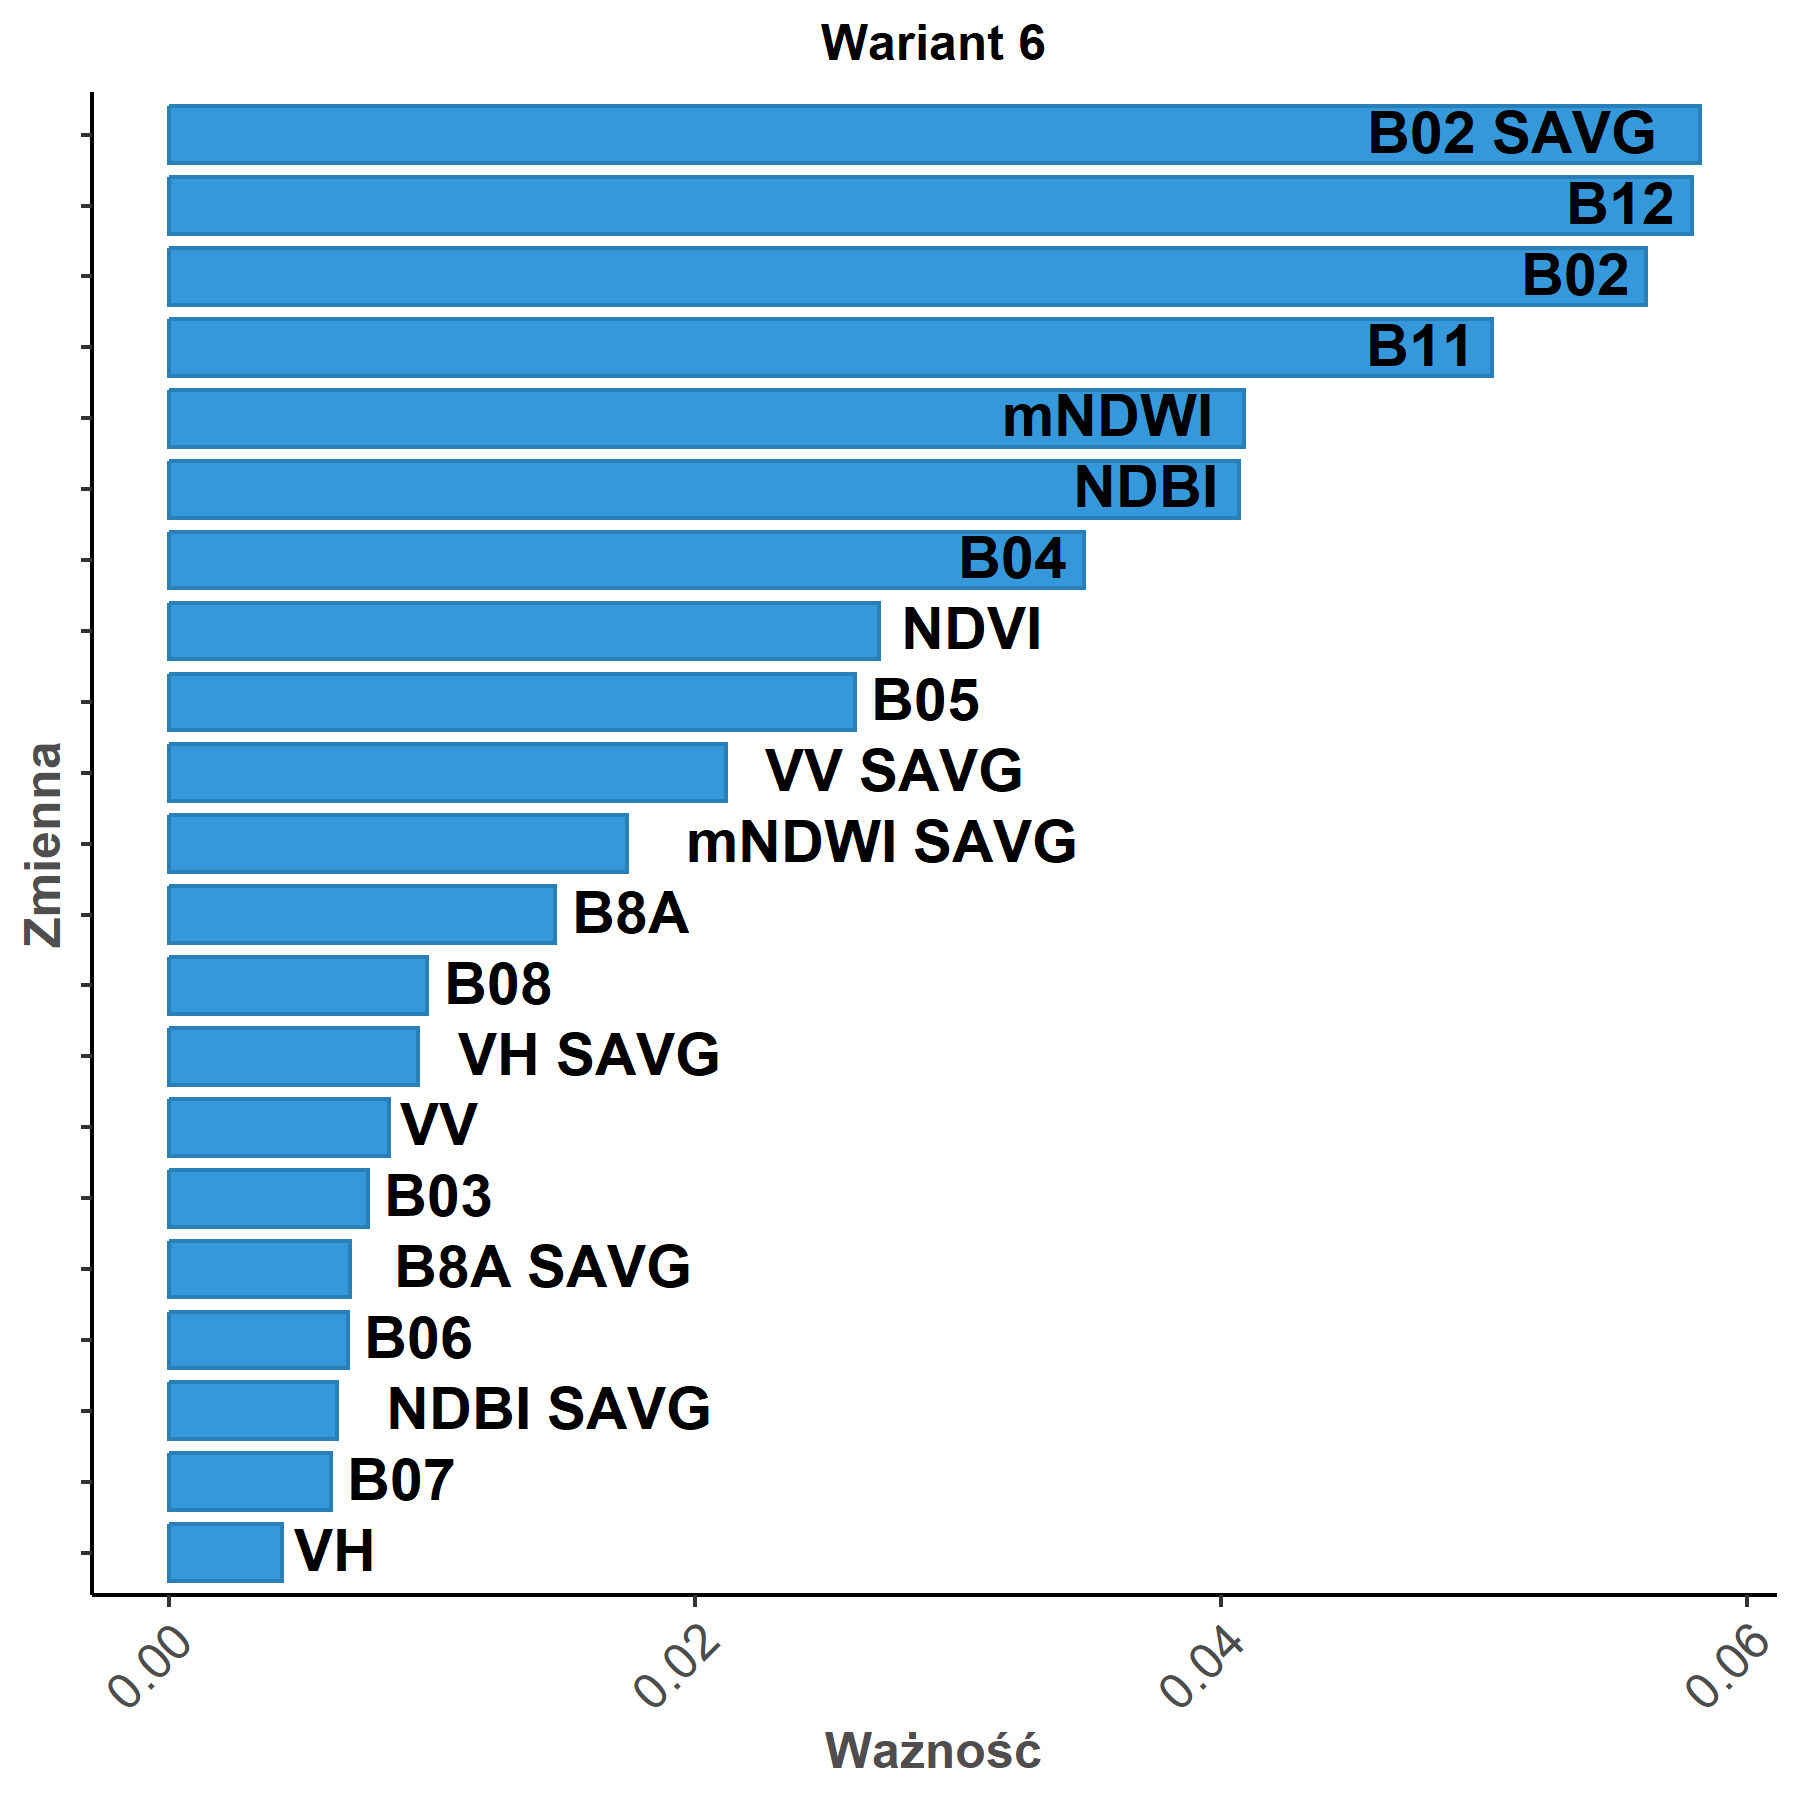
\includegraphics[width=4.6875in,height=\textheight]{figures/importance_plot_dataset6_pl.png}

}

\caption{\label{fig-rycina-variance-importance-dataset6}Permutowana
ważność zmiennych dla wariantu nr 6}

\end{figure}

Pomijając aspekt związków i interakcji pomiędzy zmiennymi, które
powodowały subtelne różnice w kolejności znaczenia zmiennych dla
poszczególnych wariantów, zauważalny jest podział zmiennych na pięć grup
według ich istotności w detekcji farm fotowoltaicznych. Z rycin
\ref{fig-rycina-variance-importance_cowplot} i
\ref{fig-rycina-variance-importance-dataset6} wynika, że największe
znaczenie spośród wszystkich predyktorów miała grupa czterech zmiennych:
tekstura średniej sumy kanału niebieskiego (B02 SAVG), kanały średniej
podczerwieni (SWIR1 (B11) i SWIR2 (B12)) oraz kanał niebieski (B02).
Trochę niższą istotność w kontekście wykrywania farm fotowoltaicznych
miały trzy kolejne zmienne: znormalizowany zmodyfikowany różnicowy
wskaźnik wody (mNDVI), znormalizowany różnicowy wskaźnik obszarów
zabudowanych (NDBI) oraz kanał czerwony (B04). Trzecią grupę stanowiły
dwie zmienne: znormalizowany różnicowy wskaźnik wegetacji (NDVI) oraz
jeden z kanałów czerwieni krawędziowej (tzw. \emph{RedEdge}, B05), a do
czwartej grupy zaliczyć można tekstury średniej sumy dla polaryzacji VV
i wskaźnika mNDWI (VV SAVG, mNDWI SAVG) oraz kanał bliskiej podczerwieni
(B8A). Najmniejsze znaczenie przy detekcji farm fotowoltaicznych miały
kanał zielony (B03), pozostałe kanały czerwieni krawędziowej (B06 i
B07), kanał bliskiej podczerwieni (B08), obie wykorzystane polaryzacje
(VV i VH) oraz tekstury średniej sumy dla kanału B8A, polaryzacji VH
oraz wskaźnika NDBI (B8A SAVG, VH SAVG i NDBI SAVG).

Uzyskane wyniki oceny ważności zmiennych wskazują na dość spore znacznie
wskaźników spektralnych, głównie mNDWI oraz NDBI w kontekście wykrywania
farm fotowoltaicznych. Niskie znaczenie w tym zastosowaniu wykazują
natomiast dane radarowe pochodzące z misji Sentinel-1 oraz tekstury
średniej sumy dla tych zmiennych.

Spośród sześciu obliczonych tekstur średniej sumy wskazanych przez Wanga
et al. \autocite*{wang_2022_pv} jako istotne przy detekcji farm
fotowoltaicznych na podstawie danych Sentinel-1, Sentinel-2 i algorytmu
Random Forest, jedynie tekstura średniej sumy dla kanału niebieskiego
wykazywała się znaczącym wpływem na wynik klasyfikacji. Pozostałe
tekstury wskazywały przeciętną lub niską istotność w tym konkretnym
zadaniu. Ważność trzech z obliczonych tekstur (B02 SAVG, VV SAVG i VH
SAVG) była wyższa niż ocena ważności odpowiadających im danych
pierwotnych. W przypadku pozostałych trzech tekstur (B8A SAVG, mNDWI
SAVG i NDBI SAVG), uzyskane wyniki były niższe niż wyniki pierwotnych
danych teledetekcyjnych.

\begin{figure}[t]

{\centering 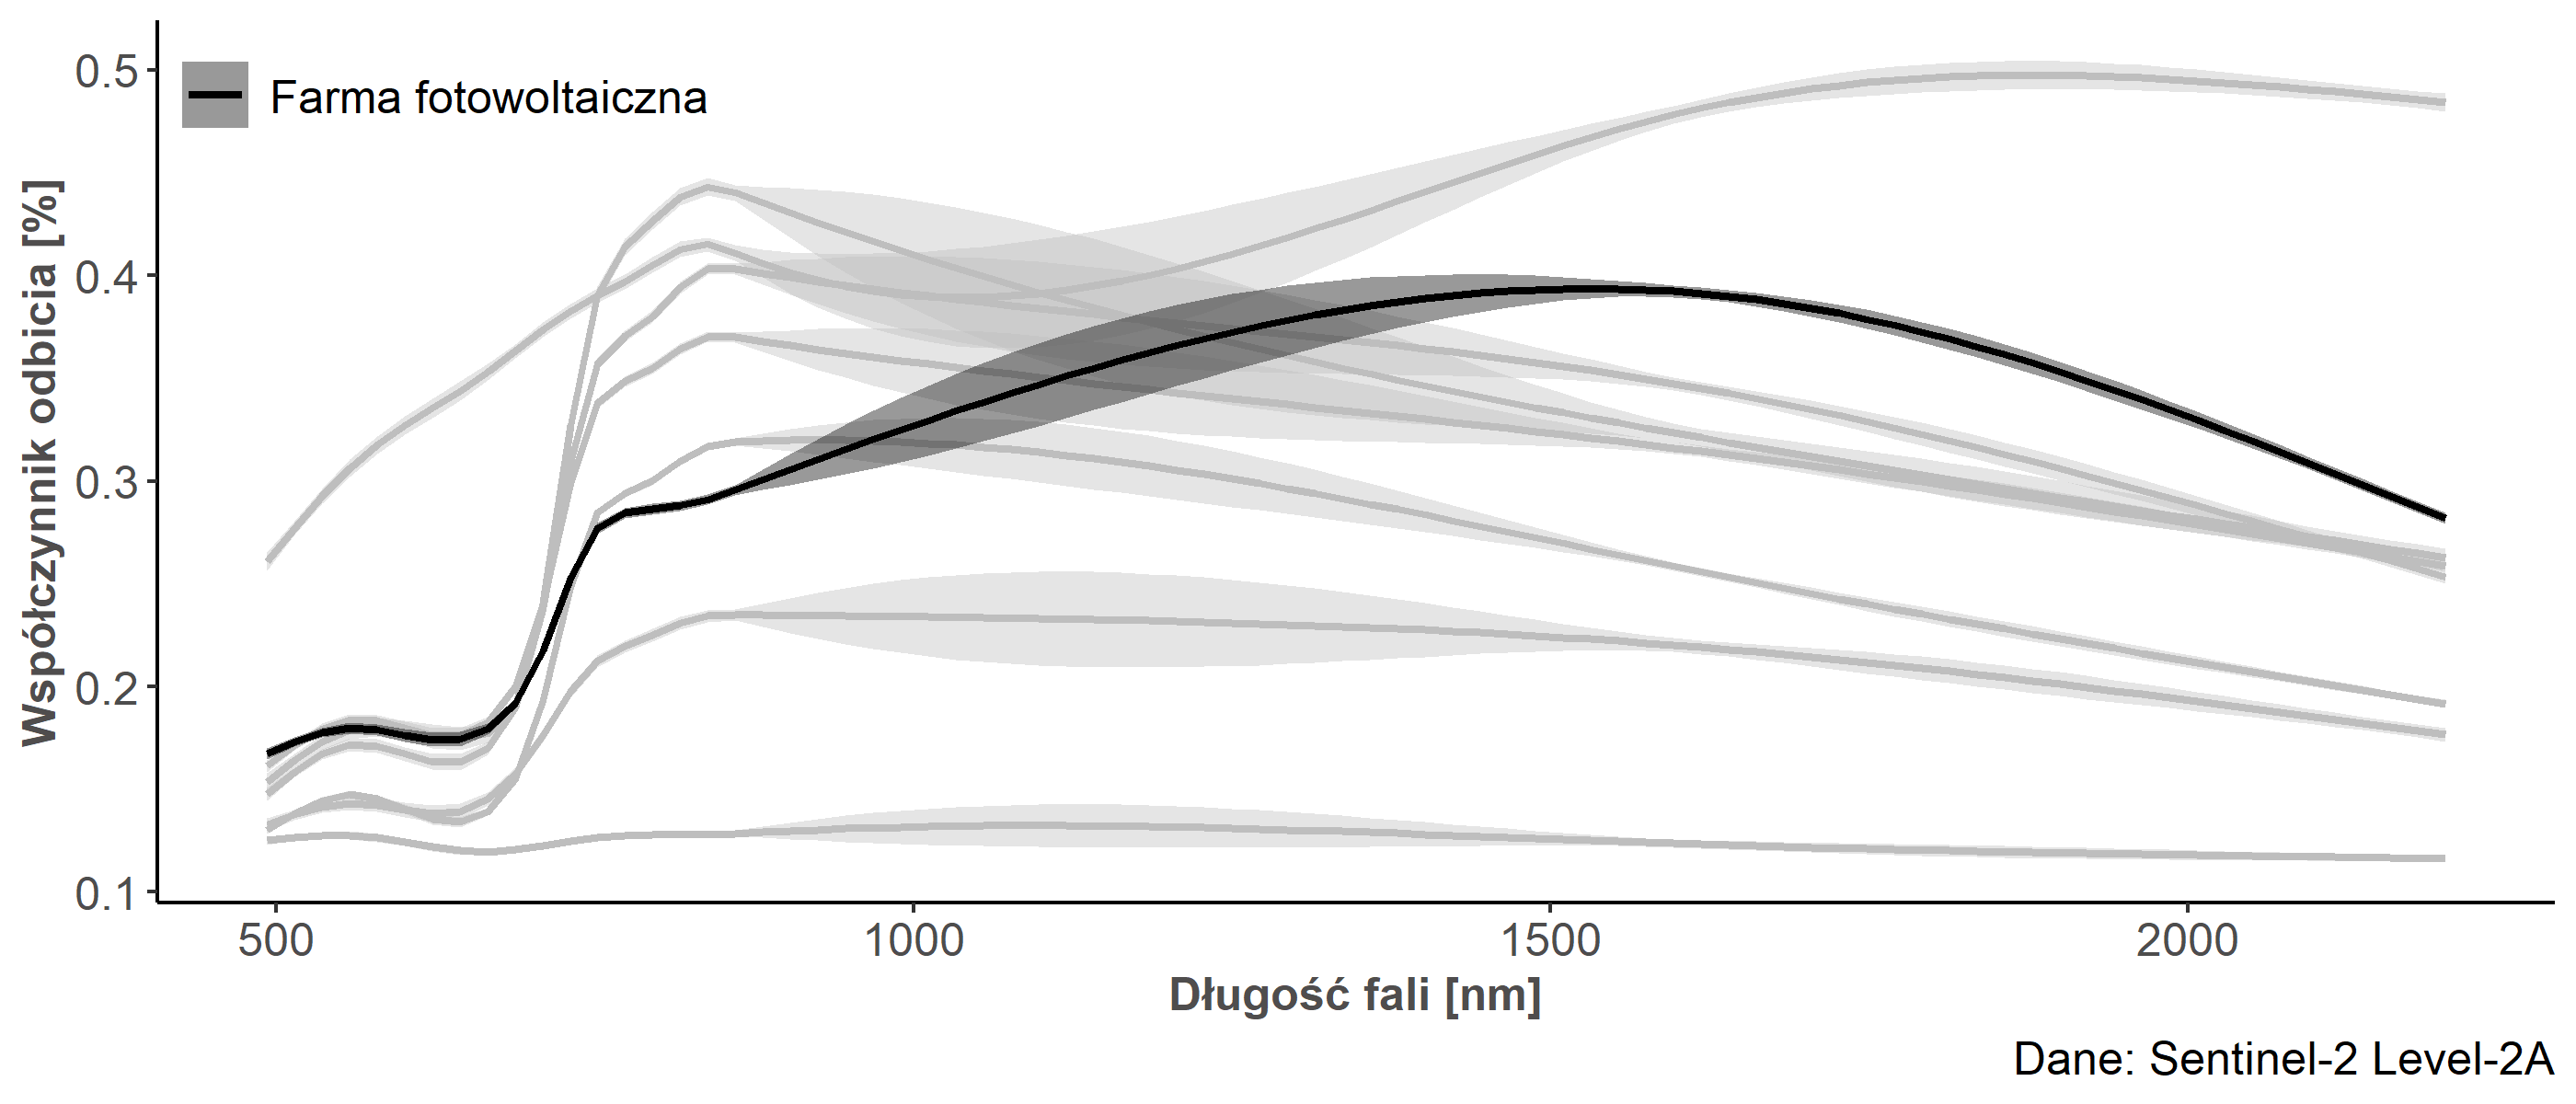
\includegraphics[width=1\textwidth,height=\textheight]{figures/spectral_curves_plot2.png}

}

\caption{\label{fig-rycina-spectral-curves}Krzywa odbicia spektralnego
farm fotowoltaicznych na tle innych typów pokrycia terenu}

\end{figure}

Charakterystyka spektralna farm fotowoltaicznych (rycina
\ref{fig-rycina-spectral-curves}) wyjaśnia znaczenie kanałów B02, B11 i
B12 w kontekście detekcji farm fotowoltaicznych na podstawie danych
teledetekcyjnych. Krzywa spektralna instalacji fotowoltaicznych wskazuje
na spektralne zróżnicowanie tej powierzchni względem innych typów
pokrycia terenu w zakresie pasm średniej podczerwieni, do których należą
kanały B11 (1610 nm) i B12 (2190 nm). Farmy fotowoltaiczne
charakteryzują się wyższym współczynnikiem odbicia od większości innych
powierzchni w zakresie fal niebieskich (kanał B02, 493 nm). Oznacza to,
że odpowiedź spektralna instalacji fotowoltaicznych w tym zakresie
różnicuje je od innych typów pokrycia terenu.

\hypertarget{sec-classification-results}{%
\section{Wyniki klasyfikacji po przetwarzaniu
końcowym}\label{sec-classification-results}}

Sekcja \ref{sec-results-model-quality-assessment} omawiała wyniki
jakości klasyfikacji na podstawie próby, a wyniki oceny jakości modelu
uzyskane na niewielkiej części populacji mogą znacznie różnić się od
rezultatów uzyskanych podczas klasyfikacji całej populacji, obejmującej
wszystkie obserwacje na badanym obszarze.

W celu oceny rzeczywistej jakości klasyfikacji dla całej populacji po
procesie przetwarzania końcowego dokonano porównania wyników predykcji
każdego wariantu (tabela \ref{tbl-tabela-datasets}) ze zbiorem
referencyjnym. Referencyjny zbiór danych obejmował wszystkie farmy
fotowoltaiczne, które udało się określić na obszarze kafla Sentinel-2 o
oznaczeniu 33UWV w czasie wykonywania użytych zobrazowań (8 maja 2023
roku). Dane te zostały zdigitalizowane na podstawie ortofotomapy oraz
mozaik satelitarnych. Porównanie wymagało przekształcenia
zdigitalizowanych farm fotowoltaicznych do postaci rastrowej, przyjmując
siatkę 10-metrowych kanałów wykorzystanej sceny Sentinel-2.

Wyniki klasyfikacji dotyczące liczby wykrytych farm fotowoltaicznych lub
ich oddzielnych segmentów oraz sumy wykrytej powierzchni po procesie
przetwarzania końcowego zostały przedstawione w tabeli
\ref{tbl-tabela-classification-results}. Pierwszy wiersz odnosi się do
zbioru referencyjnego, który obejmował wszystkie farmy fotowoltaiczne
określone na obszarze kafla Sentinel-2 o oznaczeniu 33UWV w czasie
wykonania użytych zobrazowań (8 maja 2023 roku).

\hypertarget{tbl-tabela-classification-results}{}
\begin{table}
\caption{\label{tbl-tabela-classification-results}Wyniki klasyfikacji uzyskane po procesie przetwarzania końcowego }\tabularnewline

\centering
\begin{tabular}{>{\centering\arraybackslash}p{3.4cm}>{\centering\arraybackslash}p{3cm}>{\centering\arraybackslash}p{3cm}>{\centering\arraybackslash}p{4cm}}
\toprule
Wariant \textsuperscript{a} & Liczba wykrytych poligonów & Suma wykrytej powierzchni [ha] & Poprawnie wykryta powierzchnia farm na podstawie macierzy pomyłek [ha]\\
\midrule
Zbiór referencyjny \textsuperscript{b} & 210 & 345.04 & -\\
1 & 650 & 516.57 & 290.86\\
2 & 263 & 335.71 & 291.01\\
3 & 294 & 344.28 & 289.30\\
4 & 733 & 487.05 & 287.24\\
5 & 505 & 406.26 & 286.29\\
6 & 323 & 394.95 & 291.10\\
\bottomrule
\multicolumn{4}{l}{\textsuperscript{a} Patrz: tabela 4.1}\\
\multicolumn{4}{l}{\textsuperscript{b} Zdigitalizowane farmy fotowoltaiczne na podstawie ortofotomapy i mozaik satelitarnych}\\
\end{tabular}
\end{table}

Analiza wyników w tabeli wskazuje na znaczne zróżnicowanie zarówno pod
względem liczby wykrytych poligonów (odpowiadających poszczególnym
segmentom farm fotowoltaicznych), jak i sumy wykrytej powierzchni.
Warianty nr 2 i 3 osiągnęły wyniki najbardziej zbliżone do
rzeczywistych, prezentując zbliżoną sumę powierzchni wskazanej jako
farmy fotowoltaiczne. Niemniej jednak oba warianty różnią się znacząco
pod względem liczby wykrytych poligonów.

Pod względem poprawnie wykrytej powierzchni elektrowni fotowoltaicznych,
ustalonej na podstawie macierzy pomyłek, wyniki poszczególnych wariantów
są stosunkowo zbliżone i mieszczą się w zakresie od 286,29 ha do 291,10
ha. Wariant nr 6 okazał się najlepszy pod względem wykrytej powierzchni,
natomiast najgorszy wynik uzyskał wariant nr 5.

Warto jednak zaznaczyć, że wyniki predykcji po etapie przetwarzania
końcowego są dość mocno niekompletne, ponieważ każdemu z wariantów
brakuje około 55 ha powierzchni farm fotowoltaicznych względem zbioru
referencyjnego. Wartość ta stanowi ponad 15\% powierzchni elektrowni
fotowoltaicznych na obszarze badań i sygnalizuje pewne ograniczenia w
skuteczności klasyfikacji.

\begin{figure}[t]

{\centering 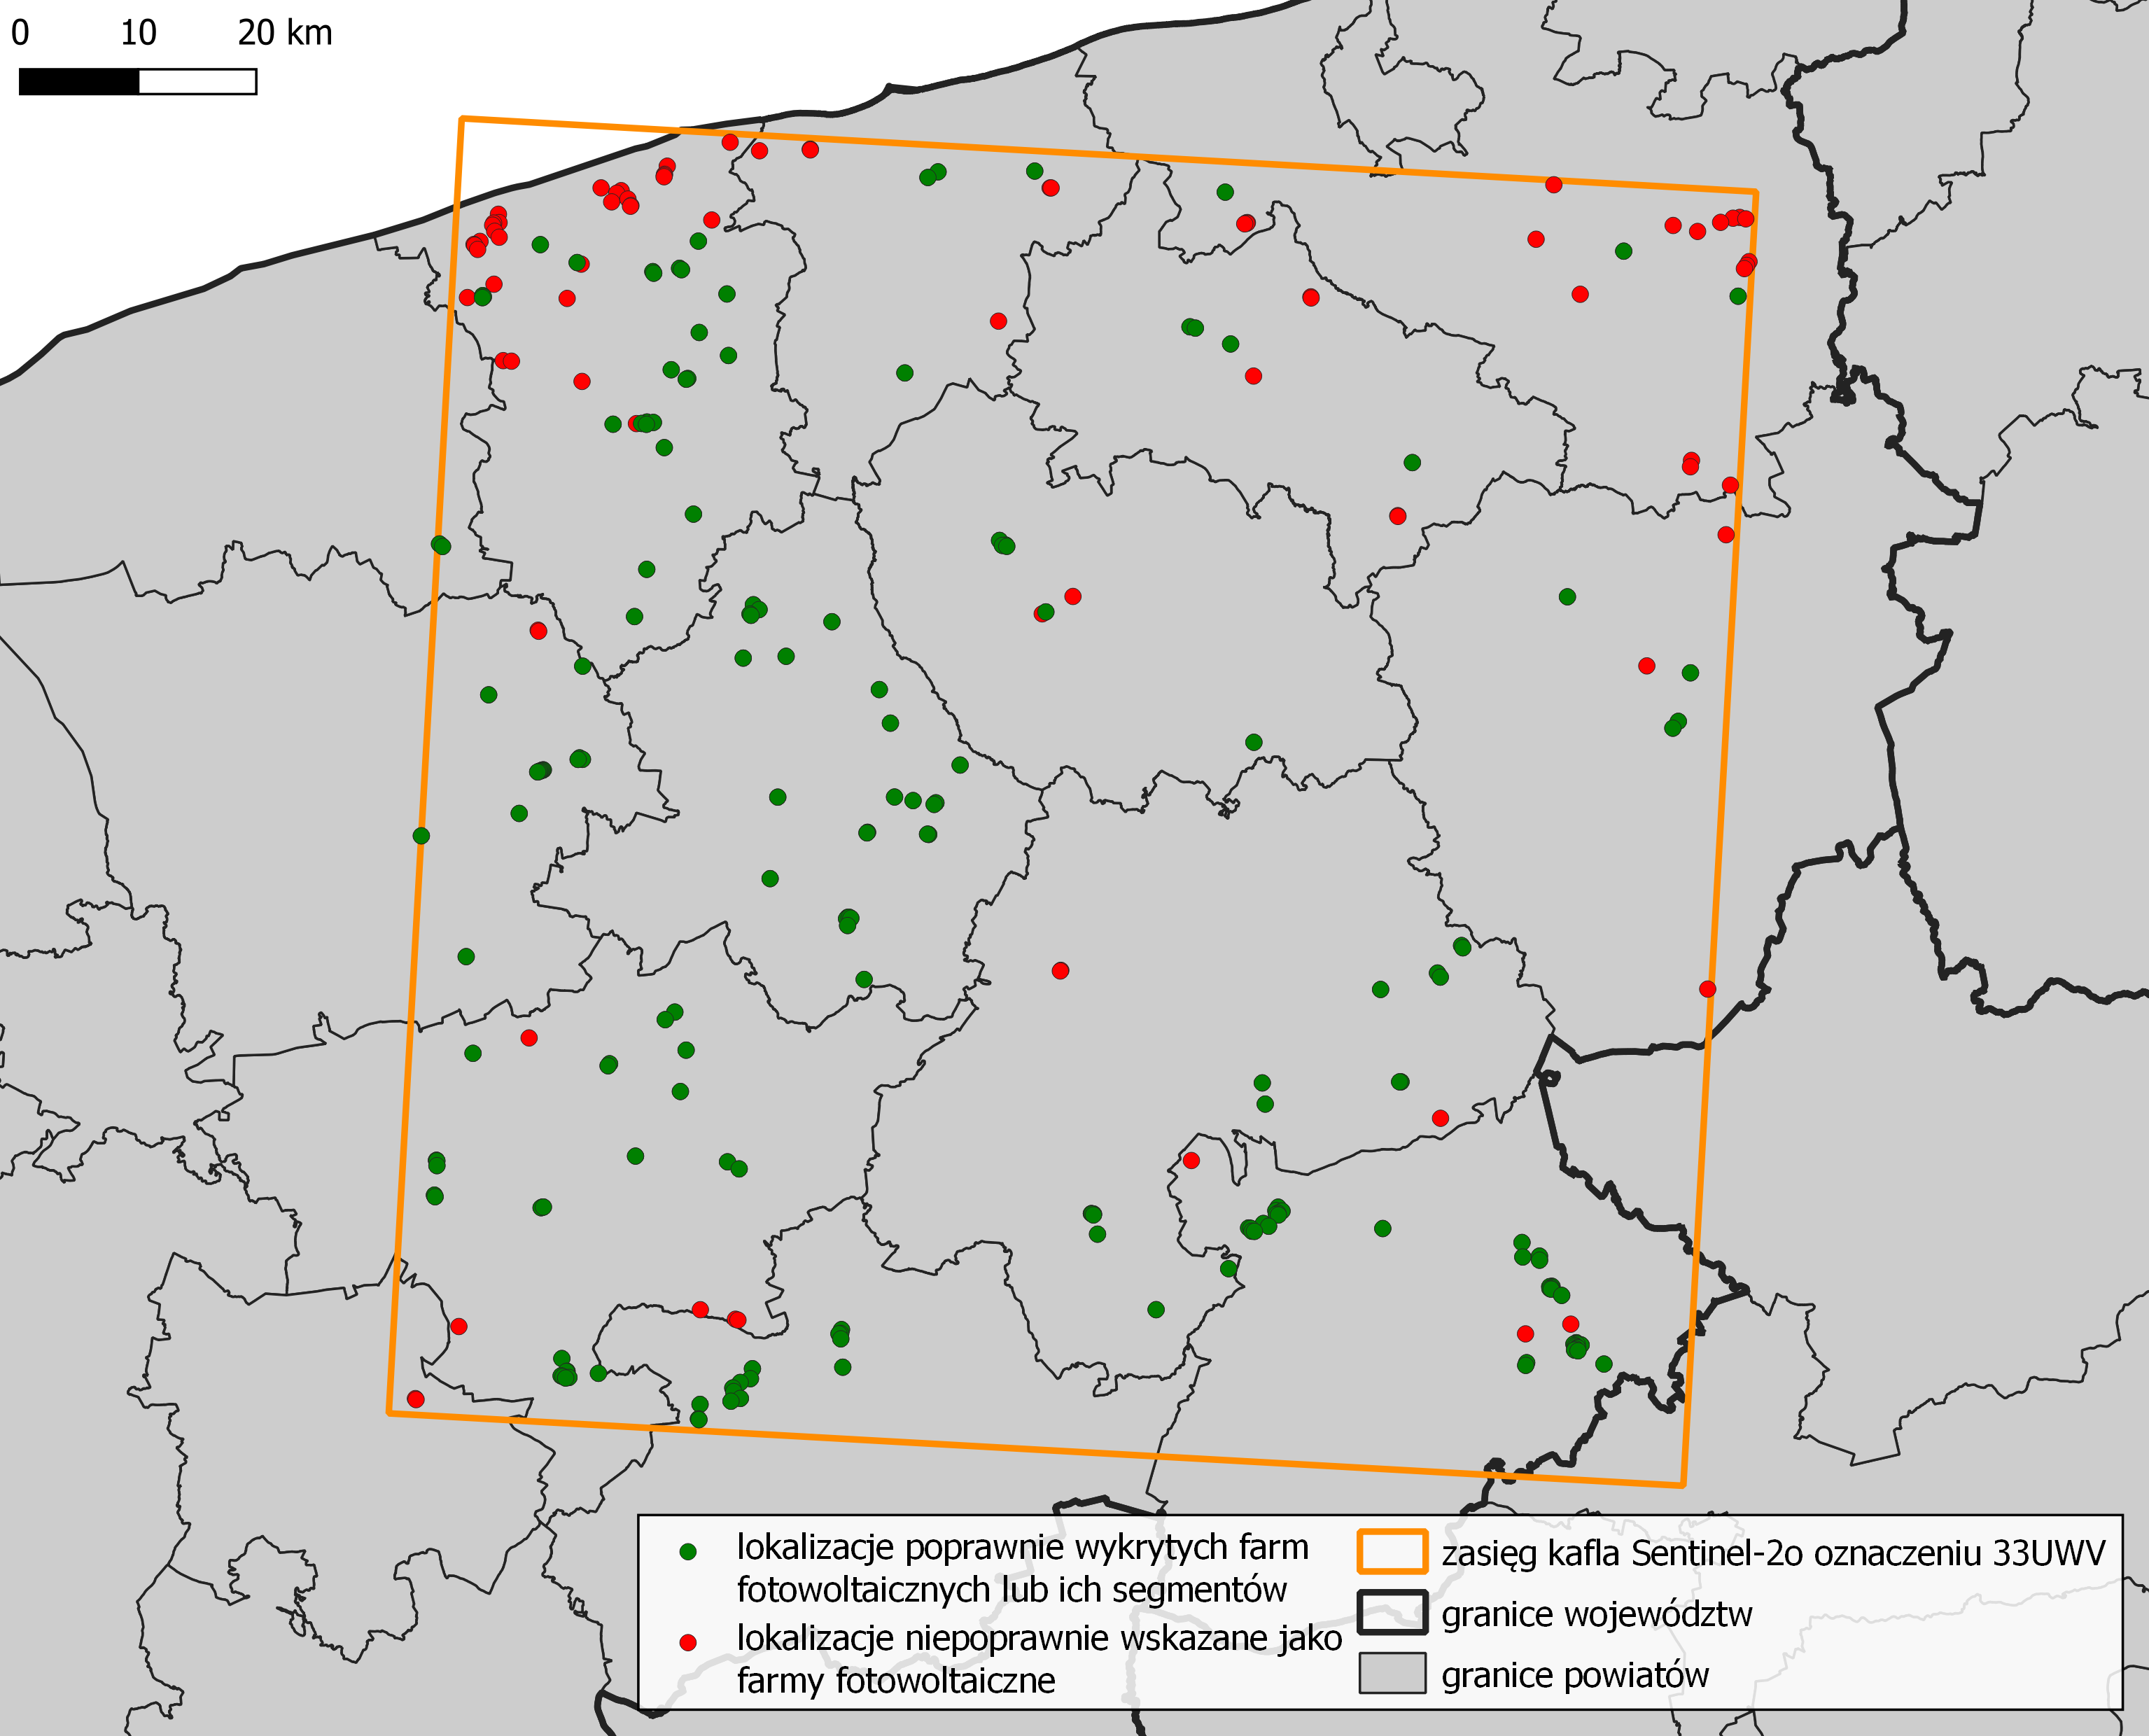
\includegraphics[width=1\textwidth,height=\textheight]{figures/poprawne_niepoprawne_wskazania_dataset2.png}

}

\caption{\label{fig-rycina-classification-results-dataset2}Lokalizacje
poprawnie i niepoprawnie wykrytych farm fotowoltaicznych lub ich
segmentów dla wariantu nr 2}

\end{figure}

Rozmieszczenie poprawnie i niepoprawnie wykrytych farm fotowoltaicznych
dla wariantu drugiego przedstawia rycina
\ref{fig-rycina-classification-results-dataset2}. Z ilustracji wynika,
że większość elektrowni fotowoltaicznych lub ich segmentów została
właściwie zidentyfikowana, a błędnie sklasyfikowane lokalizacje farm
fotowoltaicznych występują głównie w północnej części badanego obszaru.
Niewłaściwe wskazania w północno-zachodniej części obszaru badań
koncentrują się głównie na obszarach łąk, pastwisk oraz nieużytków,
szczególnie tam, gdzie występuje gęsta sieć melioracyjna, podczas gdy
błędne lokalizacje farm fotowoltaicznych w części północno-wschodniej
związane są głównie z predykcjami występującymi na obszarach
zachmurzonych.

\hypertarget{sec-population-quality-assessment}{%
\subsection{Ocena jakości klasyfikacji dla
populacji}\label{sec-population-quality-assessment}}

Ocena jakości klasyfikacji dla całego obszaru badań (populacji) została
przeprowadzona zgodnie z podejściem opisanym w sekcji
\ref{sec-model-quality-assessment}. Wykorzystane podejście, podobnie jak
ocena jakości modeli, opiera się na analizie macierzy błędów, która
umożliwiła obliczenie trzech miar jakości: precyzji, czułości oraz
F1-score.

\hypertarget{tbl-tabela-population-quality-assessment}{}
\begin{table}
\caption{\label{tbl-tabela-population-quality-assessment}Wyniki oceny jakości klasyfikacji uzyskane dla całej populacji }\tabularnewline

\centering
\begin{tabular}{cccc}
\toprule
Wariant \textsuperscript{a} & Precyzja & Czułość & F1-score\\
\midrule
1 & 0.5631 & 0.8414 & 0.6747\\
2 & 0.8668 & 0.8419 & 0.8542\\
3 & 0.8403 & 0.8369 & 0.8386\\
4 & 0.5898 & 0.8310 & 0.6899\\
5 & 0.7047 & 0.8282 & 0.7615\\
6 & 0.7371 & 0.8421 & 0.7861\\
\bottomrule
\multicolumn{4}{l}{\textsuperscript{a} Patrz: tabela 4.1}\\
\end{tabular}
\end{table}

Wyniki oceny jakości klasyfikacji dla populacji każdego wariantu
przedstawia tabela \ref{tbl-tabela-population-quality-assessment}, która
wskazuje na znaczne rozbieżności w kontekście precyzji. Precyzja ocenia
w pewnym sensie skłonność modelu do przeuczania się, określając jaka
część wyników wskazanych przez klasyfikator jako pozytywne jest
faktycznie pozytywne w rzeczywistości. Przeuczanie występuję w sytuacji,
gdy klasyfikator wskazuje farmy fotowoltaiczne w miejscach, gdzie
faktycznie one nie występowały. Najlepszą precyzję osiągnęły warianty nr
2 i 3, gdzie wartości tej miary wynoszą odpowiednio 0,8668 i 0,8403.
Warianty nr 4 i 1 prezentują natomiast niską precyzję, wynoszącą
odpowiednio 0,5898 i 0,5631, co sugeruje duże przeuczenie tych dwóch
klasyfikatorów. Wyniki precyzji poniżej wartości 0,60 wskazują, że ponad
40\% obszarów wskazanych jako farmy fotowoltaiczne w rzeczywistości nimi
nie jest. Oba warianty z najniższymi wynikami precyzji oparte były
wyłącznie na pierwotnych danych teledetekcyjnych. Wariant nr 1 składał
się wyłącznie ze zmiennych będących reflektancją kanałów Sentinel-2,
natomiast wariant nr 4 oprócz reflektancji zawierał surowe dane o
współczynniku rozproszenia wstecznego dla obu polaryzacji Sentinel-1.
Wyniki wariantów zawierających pochodne danych teledetekcyjnych
(wskaźniki teledetekcyjne, tekstury obrazu) uzyskały znacznie wyższe
wyniki precyzji, co wskazuje na duże znaczenie informacji pochodnej w
kontekście wykrywania farm fotowoltaicznych na podstawie danych
teledetekcyjnych. Sugeruje to, że wykorzystanie danych pochodnych
zmniejsza tendencję modeli do przeuczania, jednak należy zauważyć, że
wariant zawierający wszystkie zmienne pochodne nie uzyskał najlepszych
wyników precyzji.

W zakresie czułości wyniki są znacznie mniej zróżnicowane, utrzymując
się między 0,8282 a 0,8421. Czułość określa, jaką część rzeczywistych
przypadków wykrył klasyfikator, czyli jaki ułamek farm znajdujących się
w referencyjnym zbiorze danych został wykryty. Najwyższy wynik czułości
osiągnął wariant nr 6, a najniższy - wariant nr 5.

Jak wspomniano w sekcji \ref{sec-model-quality-assessment}, miara
F1-score jest średnią harmoniczną precyzji i czułości, używaną, gdy obie
te miary są równie istotne. Miara F1-score opisuje całościowo wynik, a
ponieważ wyniki czułości dla poszczególnych wariantów są zbliżone do
siebie, to precyzja będzie miała kluczowy wpływ na ostateczną ocenę
jakości klasyfikacji. Najwyższym wynikiem miary F1-score charakteryzuje
się wariant nr 2 (0,8542), a próg wartości 0,80 przekroczył również
wariant nr 3. Stosując wyłącznie surowe dane teledetekcyjne, warianty nr
1 i 4 nie przekraczają progu 0,70 dla miary F1-score, podczas gdy
pozostałe warianty, zawierające dane pochodne, uzyskały znacznie wyższe
wartości.

Ogólnie rzecz biorąc, wyniki sugerują, że korzystanie z pochodnych
danych teledetekcyjnych istotnie redukuje skłonność modelu do
przeuczenia, poprawiając jednocześnie jego jakość w kontekście detekcji
farm fotowoltaicznych.

\hypertarget{sec-visual-quality-assessment}{%
\subsection{Wizualna kontrola wyników
klasyfikacji}\label{sec-visual-quality-assessment}}

Zgodnie z sekcją dotyczącą przestrzennej oceny jakości (sekcja
\ref{sec-population-quality-assessment}), modele stworzone w ramach
niniejszego badania wykazują dobrą skuteczność w identyfikacji farm
fotowoltaicznych, co ilustruje również rycina
\ref{fig-rycina-truepositive-dataset2}, przedstawiająca przykłady
poprawnych przewidywań dla wariantu nr 2 \footnote{Wyniki klasyfikacji
  tego wariantu w formie danych przestrzennych można znaleźć pod adresem
  https://github.com/filrat2/wykrywanie-farm-fotowoltaicznych-2024 .}.
Dla porównania, na rycinie przedstawiono także instalacje fotowoltaiczne
generujące energię elektryczną, pochodzące z badania przeprowadzonego
przez Kruitwagena et al. \autocite*{kruitwagen_2021_pv}, wskazującego
istniejące konstrukcje fotowoltaiczne na świecie na dzień 30 września
2018 roku. Wysokorozdzielcze obrazy satelitarne na rycinie
\ref{fig-rycina-truepositive-dataset2} (kolumna a) pochodzą z różnych
okresów. Obraz satelitarny 2a został pozyskany później niż dane użyte do
detekcji farm fotowoltaicznych w niniejszym badaniu (8 maja 2023 roku),
natomiast obrazy 4a i 4b pochodzą sprzed tego okresu.

W niektórych przypadkach wewnątrz wykrytych instalacji fotowoltaicznych
pojawiły się fałszywie negatywne predykcje (ang. \emph{false negative}),
co przedstawiają ryciny \ref{fig-rycina-truepositive-dataset2} 1c i
\ref{fig-rycina-post-processing} 2c. Na kompozycji RGB Sentinel-2 możemy
zaobserwować w miejscach tych błędnych wskazań różnice w jasności
komórek względem otaczającej instalacji fotowoltaicznej lub
zróżnicowanie powierzchni pod panelami fotowoltaicznymi. Rycina
\ref{fig-rycina-truepositive-dataset2} 5c pokazuje, że w niektórych
przypadkach poprawne wskazania powierzchni farm fotowoltaicznych są
niepełne, pomimo jednolitego wyglądu instalacji na kompozycji RGB
Sentinel-2.

Problemem stworzonych modeli jest ich tendencja do przeuczania się na
niektórych typach pokrycia terenu i użytkowania ziemi, co zostało
szerzej opisane w sekcji dotyczącej losowania próbek (sekcja
\ref{sec-samples}). Zaproponowane metody przetwarzania końcowego,
omówione w sekcji \ref{sec-post-processing}, poprawiają wyniki
predykcji. Niemniej jednak, w zależności od wariantu, nadal występują
mniejsze lub większe błędy w klasyfikacji. Przykłady fałszywie
pozytywnych przewidywań (ang. \emph{false positive}) zostały
przedstawione na rycinach \ref{fig-rycina-falsepositive-dataset2} (dla
wariantu nr 2) oraz \ref{fig-rycina-post-processing} (dla wariantu nr
1). Wybrane lokalizacje ilustrują typowe błędy modeli na różnych typach
pokrycia terenu i użytkowania ziemi.

Mimo zastosowania dodatkowych próbek negatywnych na drogach, jak
wskazano w sekcji \ref{sec-samples}, błędne pozytywne przewidywania w
tych miejscach nadal występują, co ilustruje pierwszy rząd ryciny
\ref{fig-rycina-falsepositive-dataset2}. Pierwszy, drugi oraz czwarty
rząd ryciny \ref{fig-rycina-falsepositive-dataset2} oraz pierwszy rząd
ryciny \ref{fig-rycina-post-processing} pokazują natomiast, że błędne
predykcje obejmują także obszary użytków rolnych (pola uprawne, łąki i
pastwiska) oraz nieużytków, szczególnie w miejscach, gdzie istnieje
gęsta sieć melioracyjna. W wyniku klasyfikacji wariantu nr 2 pojawił się
nietypowy przypadek błędnego sklasyfikowania boiska sportowego jako
instalacji fotowoltaicznej, które ze względu na powierzchnię większą niż
1000 m\textsuperscript{2} nie zostało skorygowane przez zastosowane
metody przetwarzania końcowego. Trzeci rząd ryciny
\ref{fig-rycina-falsepositive-dataset2} oraz drugi rząd ryciny
\ref{fig-rycina-post-processing} sugerują, że błędne predykcje mogą
występować również na obszarach zachmurzonych.

Należy zaznaczyć, że pomimo wykorzystania próbek z tych samych
lokalizacji do trenowania każdego z wariantów, różne modele wykazują
zróżnicowaną skuteczność klasyfikacji w zależności od typów pokrycia
terenu i użytkowania ziemi. Jest to prawdopodobnie rezultat wpływów
różnych zmiennych, gdzie niektóre z nich wspomagały decyzje w przypadku
konkretnego typu pokrycia terenu, podczas gdy inne miały przeciwny
efekt.

\begin{figure}[t]

{\centering 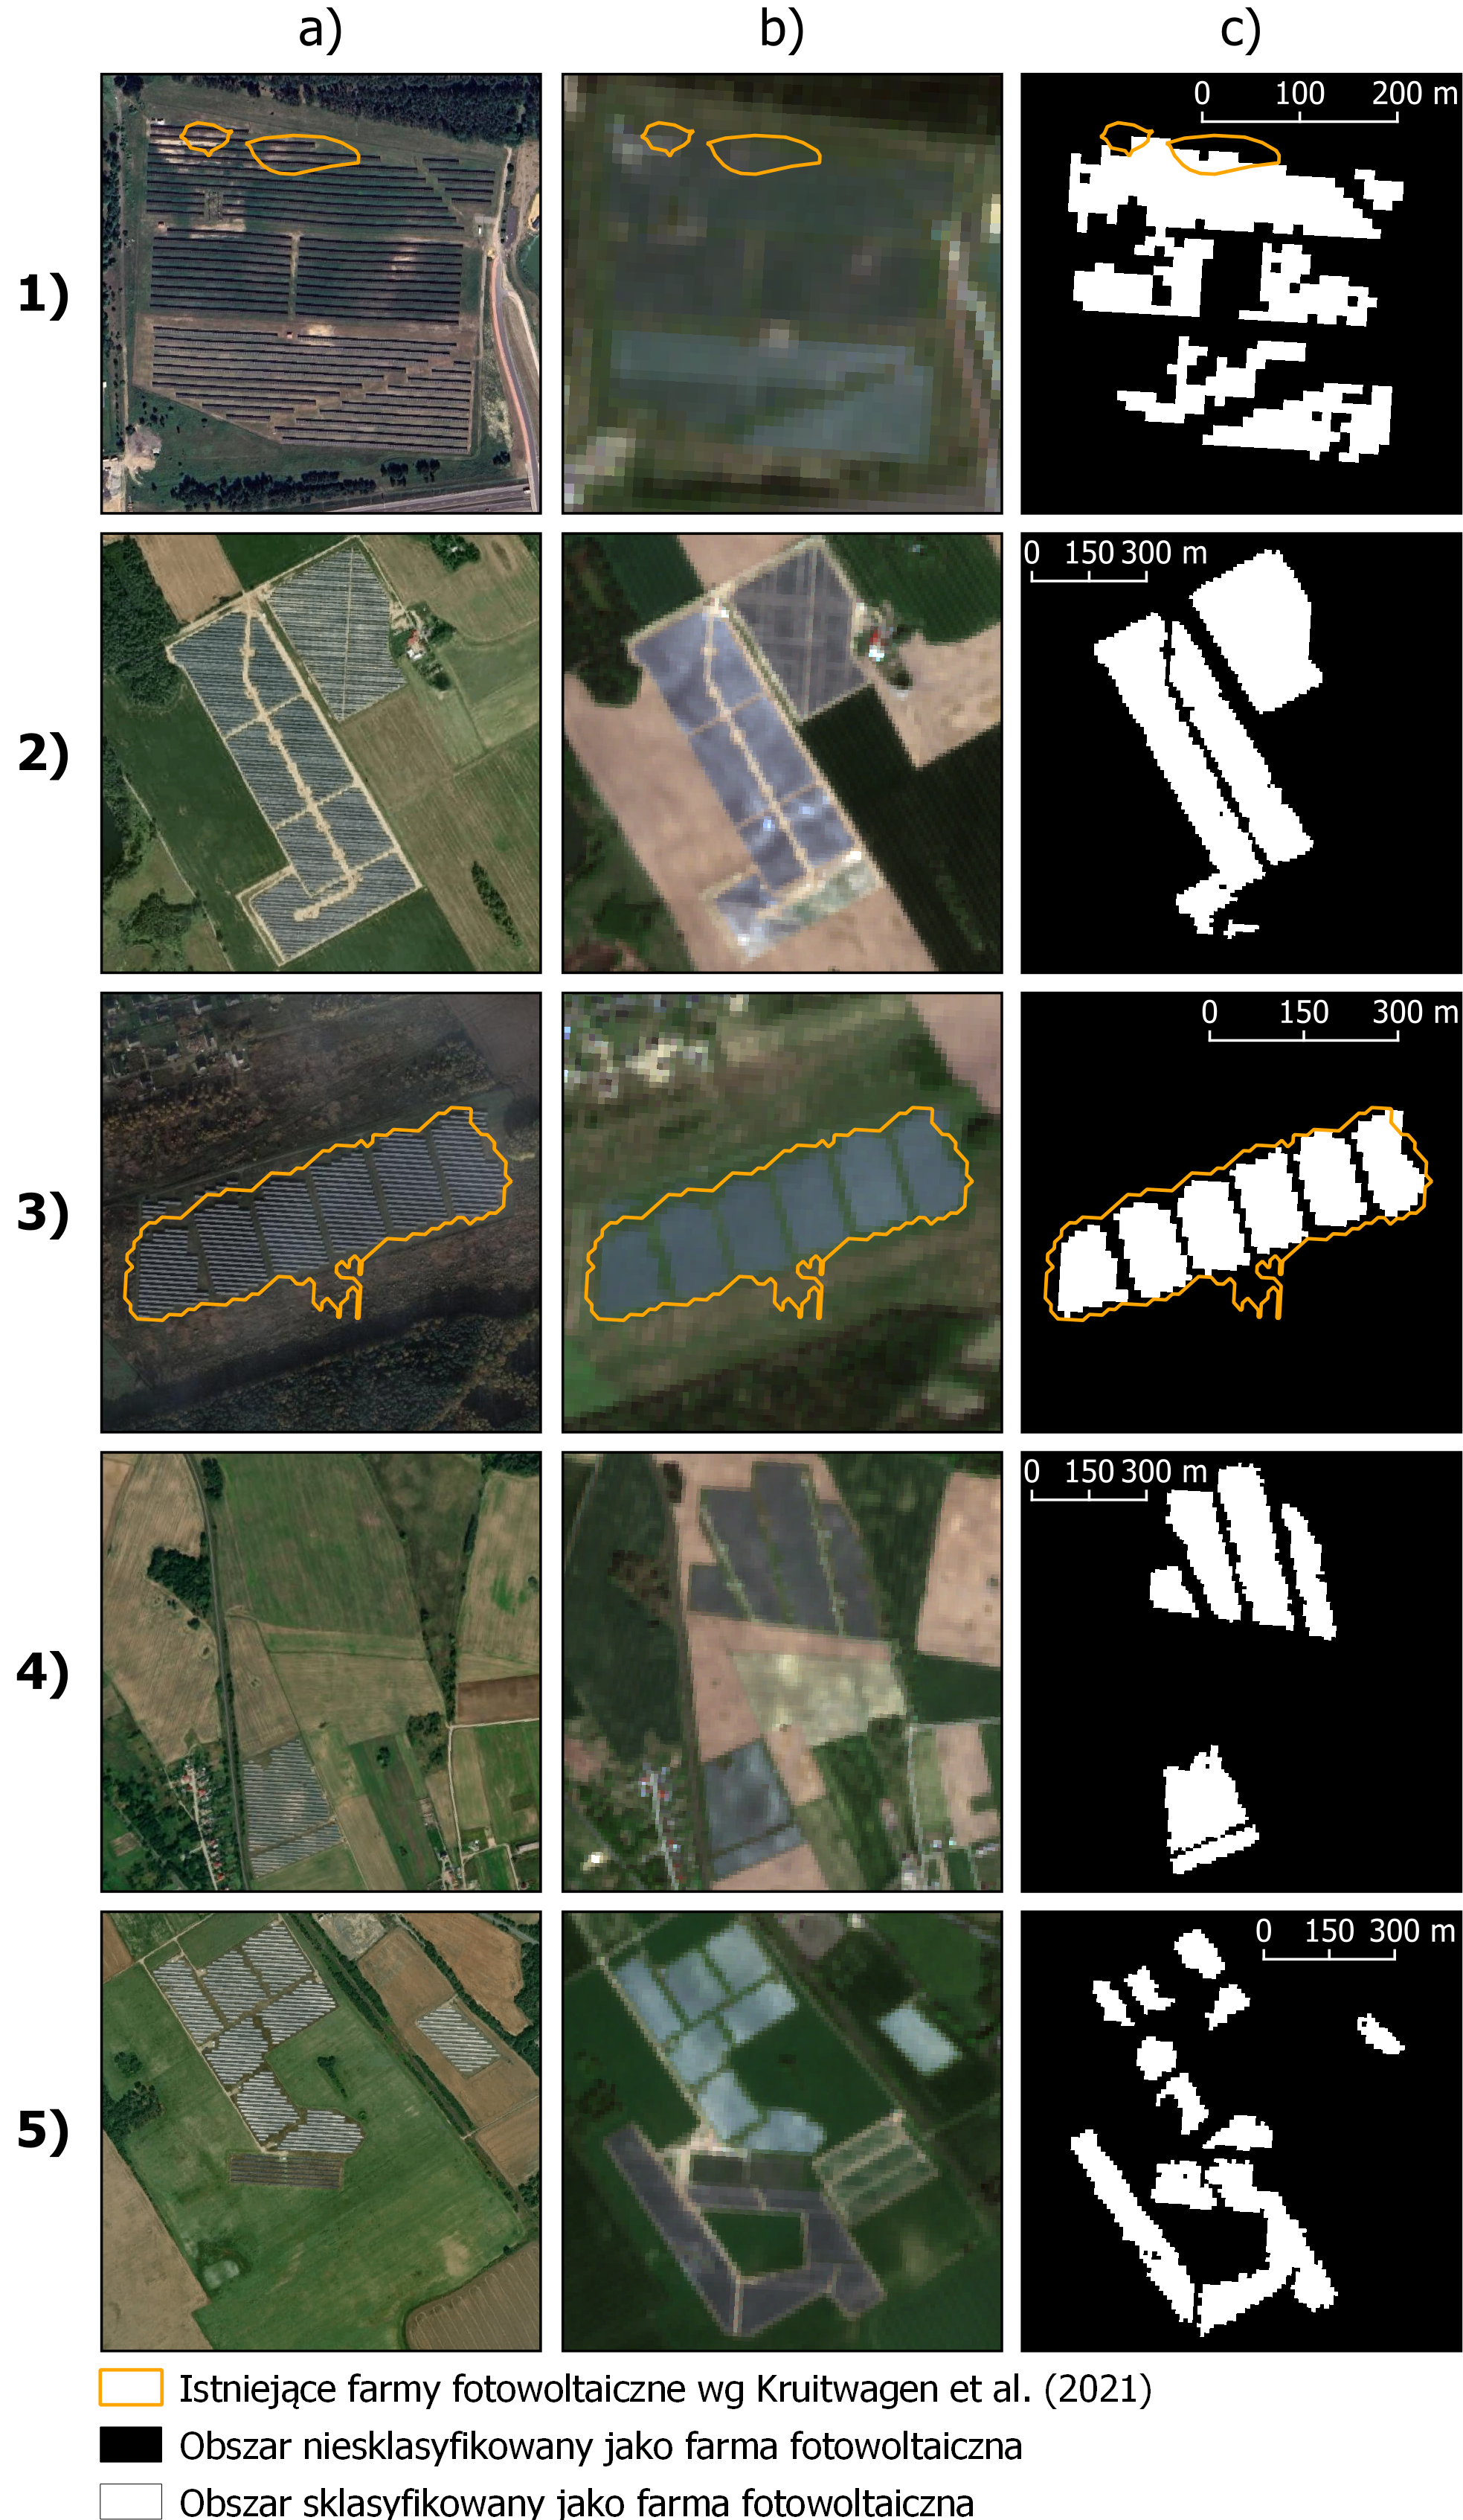
\includegraphics[width=0.87\textwidth,height=\textheight]{figures/pv_dataset2.png}

}

\caption{\label{fig-rycina-truepositive-dataset2}Wyniki klasyfikacji
wariantu nr 2 po procesie przetwarzania końcowego. Porównanie
wysokorozdzielczych obrazów satelitarnych (a) oraz kompozycji RGB
Sentinel-2 (b) z~przykładami prawdziwie pozytywnych przewidywań (ang.
true positive)}

\end{figure}

\begin{figure}[t]

{\centering 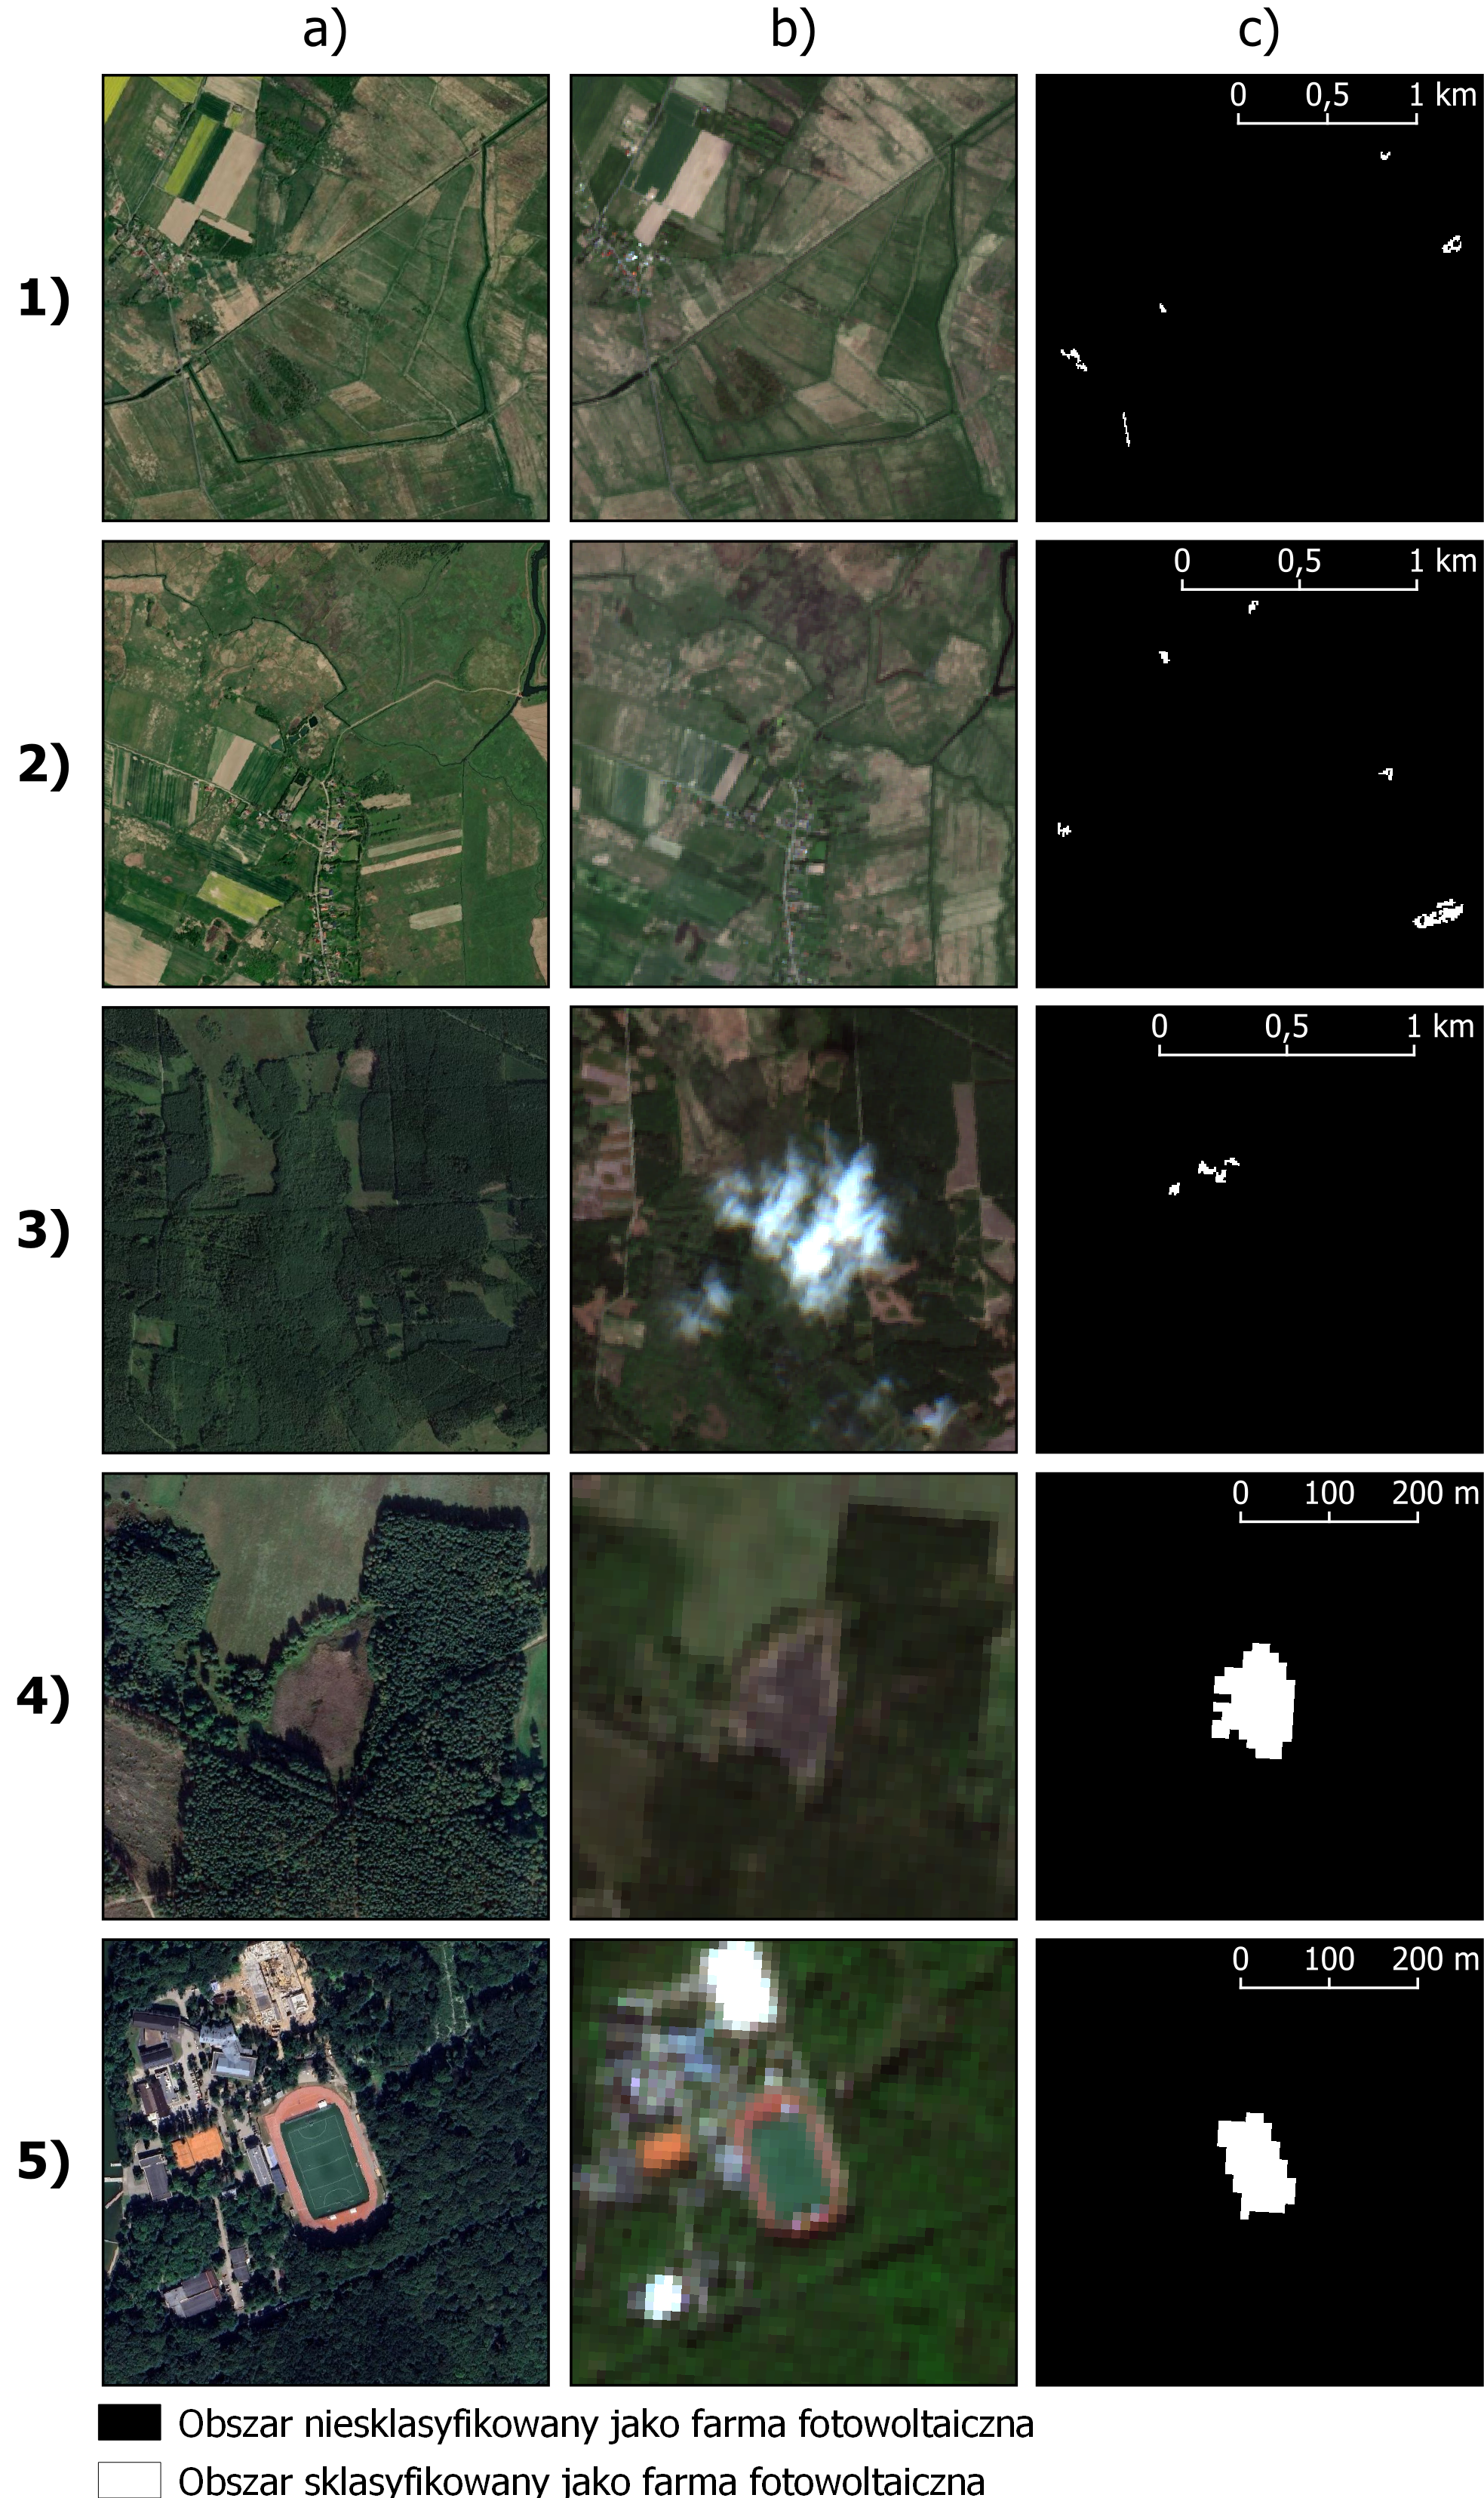
\includegraphics[width=0.89\textwidth,height=\textheight]{figures/incorrect_dataset2.png}

}

\caption{\label{fig-rycina-falsepositive-dataset2}Wyniki klasyfikacji
wariantu nr 2 po procesie przetwarzania końcowego. Porównanie
wysokorozdzielczych obrazów satelitarnych (a) oraz kompozycji RGB
Sentinel-2 (b) z~przykładami fałszywie pozytywnych przewidywań (ang.
false positive) (c)}

\end{figure}

\bookmarksetup{startatroot}

\hypertarget{podsumowanie}{%
\chapter{Podsumowanie}\label{podsumowanie}}

Badanie wykazało, że możliwe jest wykrywanie farm fotowoltaicznych na
podstawie danych teledetekcyjnych, wykorzystując do tego celu dane
satelitarne z misji Sentinel-1 i Sentinel-2. Wyniki uzyskane z wariantów
zawierających tylko pierwotne dane teledetekcyjne z tych misji uzyskały
dość przeciętne wyniki detekcji farm fotowoltaicznych. Wykorzystanie
dodatkowych zmiennych, takich jak wskaźniki teledetekcyjne czy tekstury
obrazu, istotnie poprawiło wyniki klasyfikacji. Dane radarowe z misji
Sentinel-1 i ich pochodne nie okazały się istotne w procesie detekcji
farm fotowoltaicznych. W odróżnieniu od tego, multispektralne dane z
misji Sentinel-2, wraz z ich pochodnymi, wykazały się kluczowym
elementem detekcji farm fotowoltaicznych przy wykorzystaniu danych
satelitarnych.

Optymalnym wariantem zbioru predyktorów okazał się ten składający z
kanałów Sentinel-2 oraz trzech wykorzystanych wskaźników
teledetekcyjnych (NDVI, NDBI i mNDWI), który uzyskał najwyższe wyniki
oceny jakości po ostatecznej klasyfikacji i przetwarzaniu końcowym.
Zbliżone wyniki jakości uzyskał wariant, który był rozszerzeniem
najlepszego wariantu o dodatkowe zmienne w postaci tekstur obrazu dwóch
kanałów Sentinel-2 i dwóch wskaźników teledetekcyjnych. Jeżeli dwa
klasyfikatory charakteryzują się zbliżonymi wynikami jakości, to
zazwyczaj lepszym wyborem jest ten prostszy, czyli zawierający mniej
zmiennych.

Warto zwrócić uwagę na istotne różnice między oceną jakości modeli na
próbie a ostateczną oceną klasyfikacji na całej populacji po procesie
przetwarzania końcowego. Chociaż wyniki oceny jakości modeli sugerują
bardzo zbliżoną skuteczność wszystkich modeli, to ocena przeprowadzona
na pełnej populacji ujawnia duże różnice między poszczególnymi
wariantami. Największe różnice zauważyć można w wynikach precyzji, która
ostatecznie warunkuje ostateczną ocenę jakości klasyfikatora po
przeprowadzeniu predykcji i przetwarzaniu końcowym dla każdego wariantu.
Jeśli ocena jakości modeli dla klasyfikacji nie zostałaby
przeprowadzona, moglibyśmy sądzić, że dodatkowe zmienne, czyli produkty
pochodne dostępne w poszczególnych wariantach, nie mają znaczącego
wpływu na wyniki detekcji farm fotowoltaicznych.

Z powodu nierównomiernego rozmieszczenia próbek reprezentujących farmy
fotowoltaiczne na obszarze badania, wyniki czułości oraz miary F1-score
w każdym z wariantów wykazują rozkład bimodalny. W kontekście dalszych
badań nad detekcją farm fotowoltaicznych na podstawie danych
satelitarnych warto rozważyć inne metody walidacji przestrzennej, takie
jak te sugerowane w pracy Schratza et al.
\autocite*{schratz_2022_mlr3spatiotempcv}, w celu eliminacji bimodalnego
rozkładu wyników tych miar jakości. W przypadku kontynuacji prac w tej
tematyce ważne będzie również ustawienie minimalnego odsetka obserwacji
pozytywnych w podzbiorze testowym, aby uniknąć występowania wartości
odstających w wynikach precyzji.

Porównując wyniki najlepszych wariantów z istniejącymi bazami danych
dotyczącymi elektrowni fotowoltaicznych, uzyskane wyniki są raczej
zadowalające. Globalna baza danych elektrowni (\emph{Global Power Plant
Database}) \autocite{globalpowerplantdb_2021}, stworzona przez Byersa et
al. \autocite*{byers_2018_globalpowerplantdb} i udostępniona w czerwcu
2021 roku, wskazuje na istnienie zaledwie 9 elektrowni fotowoltaicznych
w całej Polsce na wspomniany okres. Ujednolicone globalne zbiory danych
dotyczące lokalizacji farm wiatrowych i słonecznych oraz mocy
produkowanej (\emph{Harmonised global datasets of wind and solar farm
locations and power}), opracowane na podstawie danych OpenStreetMap
przez Dunnetta et al. \autocite*{dunnet_2020_wind_solar}, sugerują, że
do końca roku 2018 na obszarze badania występowały jedynie 2 instalacje
fotowoltaiczne, które zajmowały łącznie powierzchnię 1,99 hektara.
Istnieje również jeden zbiór danych, którego sposób stworzenia był
najbardziej zbliżony do omawianego w niniejszym badaniu.
\textcite{kruitwagen_2021_pv}, wykorzystując zdjęcia satelitarne
SPOT-6/7 i Sentinel-2 w połączeniu z metodami uczenia maszynowego,
wskazał istniejące konstrukcje fotowoltaiczne na świecie na dzień 30
września 2018 roku. Według wyników tego badania, na obszarze niniejszego
badania znajdowało się w tamtym momencie jedynie 10 poligonów
reprezentujących segmenty farm fotowoltaicznych o łącznej powierzchni
14,67 hektara, z czego zaledwie 8,66 ha pokrywa się z wynikami
najlepszego wariantu.

Wizualna kontrola obszarów wskazanych na rycinach potwierdziła, że
modele w większości przepadków skutecznie dokonują rozróżnienia farm
fotowoltaicznych i pozostałych obszarów podczas klasyfikacji. Niemniej
jednak, w wynikach predykcji pojawiło się kilka powtarzających się
błędów, które można częściowo wyeliminować. W celu poprawy wyników
identyfikacji farm fotowoltaicznych w kolejnych badaniach, zaleca się
zastosowanie masek eliminujących obszary chmur i ich cieni. Dodatkowo,
warto rozważyć wprowadzenie dodatkowego etapu w procesie przetwarzania
końcowego, który wykluczałby pozytywne predykcje wzdłuż dróg, zgodnie z
sugestią Ortiza et al. \autocite*{ortiz_2022_pv}.

W celu rozszerzenia obszaru detekcji farm fotowoltaicznych do obszaru
całej Polski w przyszłych badaniach, zaleca się wykorzystanie
technologii chmurowych umożliwiających przeprowadzanie analiz
geoprzestrzennych, takich jak Google Earth Engine
\autocite{gorelick_2017_gee}, Microsoft Planetary Computer
\autocite{microsoft_planetary_computer} czy openEO Platform
\autocite{openEO_platform}. Dodatkowo, wykorzystanie obliczeń w chmurze
pozwoli na rozszerzenie badania o wykorzystanie dodatkowych tekstur
obrazu, umożliwiając jednocześnie testowanie różnych konfiguracji
rozmiarów ruchomego okna i liczby poziomów kwantyzacji w celu
znalezienia optymalnych ustawień tych parametrów. Z uwagi na rosnący
czas obliczeń wraz ze zwiększaniem liczby poziomów szarości oraz
rozmiarów ruchomego okna, w niniejszej pracy nie zdecydowano się na
sprawdzenie działania innych tekstur obrazu z różnymi konfiguracjami
powyższych parametrów.

\printbibliography[heading=bibintoc, title=Bibliografia]

\end{document}
